\documentclass[twoside]{book}

% Packages required by doxygen
\usepackage{fixltx2e}
\usepackage{calc}
\usepackage{doxygen}
\usepackage{graphicx}
\usepackage[utf8]{inputenc}
\usepackage{makeidx}
\usepackage{multicol}
\usepackage{multirow}
\PassOptionsToPackage{warn}{textcomp}
\usepackage{textcomp}
\usepackage[nointegrals]{wasysym}
\usepackage[table]{xcolor}

% NLS support packages
\usepackage[french]{babel}

% Font selection
\usepackage[T1]{fontenc}
\usepackage{mathptmx}
\usepackage[scaled=.90]{helvet}
\usepackage{courier}
\usepackage{amssymb}
\usepackage{sectsty}
\renewcommand{\familydefault}{\sfdefault}
\allsectionsfont{%
  \fontseries{bc}\selectfont%
  \color{darkgray}%
}
\renewcommand{\DoxyLabelFont}{%
  \fontseries{bc}\selectfont%
  \color{darkgray}%
}
\newcommand{\+}{\discretionary{\mbox{\scriptsize$\hookleftarrow$}}{}{}}

% Page & text layout
\usepackage{geometry}
\geometry{%
  a4paper,%
  top=2.5cm,%
  bottom=2.5cm,%
  left=2.5cm,%
  right=2.5cm%
}
\tolerance=750
\hfuzz=15pt
\hbadness=750
\setlength{\emergencystretch}{15pt}
\setlength{\parindent}{0cm}
\setlength{\parskip}{0.2cm}
\makeatletter
\renewcommand{\paragraph}{%
  \@startsection{paragraph}{4}{0ex}{-1.0ex}{1.0ex}{%
    \normalfont\normalsize\bfseries\SS@parafont%
  }%
}
\renewcommand{\subparagraph}{%
  \@startsection{subparagraph}{5}{0ex}{-1.0ex}{1.0ex}{%
    \normalfont\normalsize\bfseries\SS@subparafont%
  }%
}
\makeatother

% Headers & footers
\usepackage{fancyhdr}
\pagestyle{fancyplain}
\fancyhead[LE]{\fancyplain{}{\bfseries\thepage}}
\fancyhead[CE]{\fancyplain{}{}}
\fancyhead[RE]{\fancyplain{}{\bfseries\leftmark}}
\fancyhead[LO]{\fancyplain{}{\bfseries\rightmark}}
\fancyhead[CO]{\fancyplain{}{}}
\fancyhead[RO]{\fancyplain{}{\bfseries\thepage}}
\fancyfoot[LE]{\fancyplain{}{}}
\fancyfoot[CE]{\fancyplain{}{}}
\fancyfoot[RE]{\fancyplain{}{\bfseries\scriptsize Généré le Lundi 1 Mai 2017 17\+:50\+:31 pour Damibin/\+A-\/\+Maze-\/\+Inc par Doxygen }}
\fancyfoot[LO]{\fancyplain{}{\bfseries\scriptsize Généré le Lundi 1 Mai 2017 17\+:50\+:31 pour Damibin/\+A-\/\+Maze-\/\+Inc par Doxygen }}
\fancyfoot[CO]{\fancyplain{}{}}
\fancyfoot[RO]{\fancyplain{}{}}
\renewcommand{\footrulewidth}{0.4pt}
\renewcommand{\chaptermark}[1]{%
  \markboth{#1}{}%
}
\renewcommand{\sectionmark}[1]{%
  \markright{\thesection\ #1}%
}

% Indices & bibliography
\usepackage{natbib}
\usepackage[titles]{tocloft}
\setcounter{tocdepth}{3}
\setcounter{secnumdepth}{5}
\makeindex

% Hyperlinks (required, but should be loaded last)
\usepackage{ifpdf}
\ifpdf
  \usepackage[pdftex,pagebackref=true]{hyperref}
\else
  \usepackage[ps2pdf,pagebackref=true]{hyperref}
\fi
\hypersetup{%
  colorlinks=true,%
  linkcolor=blue,%
  citecolor=blue,%
  unicode%
}

% Custom commands
\newcommand{\clearemptydoublepage}{%
  \newpage{\pagestyle{empty}\cleardoublepage}%
}


%===== C O N T E N T S =====

\begin{document}

% Titlepage & ToC
\hypersetup{pageanchor=false,
             bookmarks=true,
             bookmarksnumbered=true,
             pdfencoding=unicode
            }
\pagenumbering{roman}
\begin{titlepage}
\vspace*{7cm}
\begin{center}%
{\Large Damibin/\+A-\/\+Maze-\/\+Inc }\\
\vspace*{1cm}
{\large Généré par Doxygen 1.8.8}\\
\vspace*{0.5cm}
{\small Lundi 1 Mai 2017 17:50:31}\\
\end{center}
\end{titlepage}
\clearemptydoublepage
\tableofcontents
\clearemptydoublepage
\pagenumbering{arabic}
\hypersetup{pageanchor=true}

%--- Begin generated contents ---
\chapter{Damibin/\+A-\/\+Maze-\/\+Inc}
\label{index}\hypertarget{index}{}\hypertarget{index_intro}{}\section{Introduction}\label{index_intro}
Projet Damibin réalisé par \+: ~\newline

\begin{DoxyItemize}
\item B\+E\+N\+S\+O\+U\+S\+S\+A\+N-\/\+B\+O\+H\+M Daniel (\char`\"{}daniel.\+bensoussan-\/-\/bohm@etu.\+univ-\/lyon1.\+fr\char`\"{}) ~\newline

\item D\+O\+N\+N\+A\+Y Robin (\char`\"{}robin.\+donnay@etu.\+univ-\/lyon1.\+fr\char`\"{}) ~\newline

\item N'G\+U\+Y\+E\+N Emilien (\char`\"{}emilien.\+n'guyen@etu.\+univ-\/lyon1.\+fr\char`\"{})~\newline

\end{DoxyItemize}

Cette librairie permet de jouer au jeu A Maze Inc un plateforme/aventure/rogue-\/like ~\newline


Le code a été écrit en C++, se compile avec g++. ~\newline


Le code fonctionne normalent sous Linux et Windows, et il n'est pas nécessaire de modifier quoi que ce soit entre les deux plateformes. ~\newline


Dépendance(s) \+: ~\newline

\begin{DoxyItemize}
\item S\+D\+L2 \+: \href{http://www.libsdl.org/}{\tt http\+://www.\+libsdl.\+org/} ~\newline
 ~\newline

\end{DoxyItemize}\hypertarget{index_compil}{}\section{Pour compiler}\label{index_compil}
La compilation se fait soit avec la commande \$ make ou via codeblocks en ouvrant le projet Damibin.\+cbp puis ctrl+f11 pour recompiler tout le projet à faire seulement une fois) puis ctrl+f9. ~\newline
 Si lors de la compilation sous Windows, il y a un problème de \char`\"{}dll\char`\"{}, il faut alors copier tout les dll du dossier extern/dll/ dans bin/ ~\newline
 ~\newline
\hypertarget{index_exec}{}\section{Pour executer}\label{index_exec}
L'éxecution du jeu doit se faire dans la racine du projet puis \+: \$ ./bin/\+Jeu\+S\+D\+L, ou via codeblocks via la buildtarget Jeu\+S\+D\+L. ~\newline
 ~\newline
\hypertarget{index_doc}{}\section{Pour regénérer la documentation de code}\label{index_doc}
Dépendance \+: Doxygen \+: \href{http://www.stack.nl/~dimitri/doxygen/}{\tt http\+://www.\+stack.\+nl/$\sim$dimitri/doxygen/} ~\newline
 \$ doxygen doc/images.\+doxy ~\newline
 Puis ouvrir doc/html/index.\+html avec firefox ~\newline
 
\chapter{Index hiérarchique}
\section{Hiérarchie des classes}
Cette liste d'héritage est classée approximativement par ordre alphabétique \+:\begin{DoxyCompactList}
\item \contentsline{section}{Carte}{\pageref{classCarte}}{}
\item \contentsline{section}{Ennemis}{\pageref{classEnnemis}}{}
\begin{DoxyCompactList}
\item \contentsline{section}{Ennemis1}{\pageref{classEnnemis1}}{}
\end{DoxyCompactList}
\item \contentsline{section}{Equipement}{\pageref{classEquipement}}{}
\item \contentsline{section}{Heros}{\pageref{classHeros}}{}
\item \contentsline{section}{Image}{\pageref{classImage}}{}
\item \contentsline{section}{Jeu}{\pageref{classJeu}}{}
\item \contentsline{section}{Mini\+\_\+\+Carte}{\pageref{classMini__Carte}}{}
\item \contentsline{section}{Mini\+\_\+\+Jeux0}{\pageref{classMini__Jeux0}}{}
\item \contentsline{section}{Objet}{\pageref{classObjet}}{}
\item \contentsline{section}{sdl\+Jeu}{\pageref{classsdlJeu}}{}
\item \contentsline{section}{Statistiques}{\pageref{classStatistiques}}{}
\item \contentsline{section}{Win\+T\+X\+T}{\pageref{classWinTXT}}{}
\item \begin{DoxyCompactList}
\item \contentsline{section}{Ennemis1\+:\+:h}{\pageref{classEnnemis1_1_1h}}{}
\end{DoxyCompactList}
\end{DoxyCompactList}

\chapter{Index des classes}
\section{Liste des classes}
Liste des classes, structures, unions et interfaces avec une brève description \+:\begin{DoxyCompactList}
\item\contentsline{section}{\hyperlink{classCarte}{Carte} }{\pageref{classCarte}}{}
\item\contentsline{section}{\hyperlink{classEnnemis}{Ennemis} }{\pageref{classEnnemis}}{}
\item\contentsline{section}{\hyperlink{classEnnemis1}{Ennemis1} }{\pageref{classEnnemis1}}{}
\item\contentsline{section}{\hyperlink{classEquipement}{Equipement} }{\pageref{classEquipement}}{}
\item\contentsline{section}{\hyperlink{classEnnemis1_1_1h}{Ennemis1\+::h} }{\pageref{classEnnemis1_1_1h}}{}
\item\contentsline{section}{\hyperlink{classHeros}{Heros} }{\pageref{classHeros}}{}
\item\contentsline{section}{\hyperlink{classImage}{Image} \\*Pour gérer une image avec S\+D\+L2 }{\pageref{classImage}}{}
\item\contentsline{section}{\hyperlink{classJeu}{Jeu} }{\pageref{classJeu}}{}
\item\contentsline{section}{\hyperlink{classMini__Carte}{Mini\+\_\+\+Carte} }{\pageref{classMini__Carte}}{}
\item\contentsline{section}{\hyperlink{classMini__Jeux0}{Mini\+\_\+\+Jeux0} }{\pageref{classMini__Jeux0}}{}
\item\contentsline{section}{\hyperlink{classObjet}{Objet} }{\pageref{classObjet}}{}
\item\contentsline{section}{\hyperlink{classsdlJeu}{sdl\+Jeu} }{\pageref{classsdlJeu}}{}
\item\contentsline{section}{\hyperlink{classStatistiques}{Statistiques} }{\pageref{classStatistiques}}{}
\item\contentsline{section}{\hyperlink{classWinTXT}{Win\+T\+X\+T} \\*Une fenêtre texte est un tableau 2\+D de caractères }{\pageref{classWinTXT}}{}
\end{DoxyCompactList}

\chapter{Documentation des classes}
\hypertarget{classCarte}{\section{Référence de la classe Carte}
\label{classCarte}\index{Carte@{Carte}}
}


Graphe de collaboration de Carte\+:\nopagebreak
\begin{figure}[H]
\begin{center}
\leavevmode
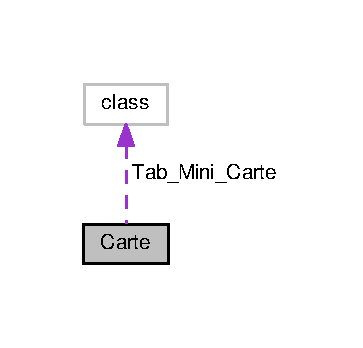
\includegraphics[width=174pt]{classCarte__coll__graph}
\end{center}
\end{figure}
\subsection*{Fonctions membres publiques}
\begin{DoxyCompactItemize}
\item 
\hypertarget{classCarte_a06daaca86c31c80f8308f4a81d46dc9b}{\hyperlink{classCarte_a06daaca86c31c80f8308f4a81d46dc9b}{Carte} ()}\label{classCarte_a06daaca86c31c80f8308f4a81d46dc9b}

\begin{DoxyCompactList}\small\item\em Constructeur par défault (pas forcément utile) \end{DoxyCompactList}\item 
\hypertarget{classCarte_a33cce3c3550977f57b0ceeb338752d58}{\hyperlink{classCarte_a33cce3c3550977f57b0ceeb338752d58}{Carte} (unsigned int nb\+X, unsigned int nb\+Y)}\label{classCarte_a33cce3c3550977f57b0ceeb338752d58}

\begin{DoxyCompactList}\small\item\em Construit le tableau de jeu de nb\+X mini carte de haut et nb\+Y mini carte de long. \end{DoxyCompactList}\item 
\hypertarget{classCarte_a63300ff55c58b5d5b1674a3fc8f25910}{\hyperlink{classCarte_a63300ff55c58b5d5b1674a3fc8f25910}{$\sim$\+Carte} ()}\label{classCarte_a63300ff55c58b5d5b1674a3fc8f25910}

\begin{DoxyCompactList}\small\item\em Destructeur. \end{DoxyCompactList}\item 
\hypertarget{classCarte_a2d0d0c093f0baf8b3e3b4602821d9e0e}{unsigned int \hyperlink{classCarte_a2d0d0c093f0baf8b3e3b4602821d9e0e}{get\+\_\+\+Tab\+\_\+\+Carte} (unsigned int x, unsigned int y) const }\label{classCarte_a2d0d0c093f0baf8b3e3b4602821d9e0e}

\begin{DoxyCompactList}\small\item\em Retourne l'entier du tableau de jeu de la xème ligne et yème colonne. \end{DoxyCompactList}\item 
\hypertarget{classCarte_a5e1d007b47aac9993874dd83dad04c6a}{void \hyperlink{classCarte_a5e1d007b47aac9993874dd83dad04c6a}{set\+\_\+\+Tab\+\_\+\+Carte} (unsigned int x, unsigned int y, unsigned int entier\+\_\+a\+\_\+mettre)}\label{classCarte_a5e1d007b47aac9993874dd83dad04c6a}

\begin{DoxyCompactList}\small\item\em Transforme l'entier de la xème ligne et yème colonne en entier\+\_\+a\+\_\+mettre. \end{DoxyCompactList}\item 
\hypertarget{classCarte_a9421170d4a06210f042763050b993cb4}{void \hyperlink{classCarte_a9421170d4a06210f042763050b993cb4}{get\+\_\+\+Tab\+\_\+\+Mini\+\_\+\+Carte} (unsigned int x, unsigned int y, class \hyperlink{classMini__Carte}{Mini\+\_\+\+Carte} \&mc)}\label{classCarte_a9421170d4a06210f042763050b993cb4}

\begin{DoxyCompactList}\small\item\em Met dans mc la mini carte du tableau de la xème ligne et yème colonne. \end{DoxyCompactList}\item 
\hypertarget{classCarte_a07a8f38a6629e2bfb0f7848d6a2aac79}{void \hyperlink{classCarte_a07a8f38a6629e2bfb0f7848d6a2aac79}{set\+\_\+\+Tab\+\_\+\+Mini\+\_\+\+Carte} (unsigned int x, unsigned int y, const class \hyperlink{classMini__Carte}{Mini\+\_\+\+Carte} \&mc)}\label{classCarte_a07a8f38a6629e2bfb0f7848d6a2aac79}

\begin{DoxyCompactList}\small\item\em Transforme la mini carte de la xème ligne et yème colonne en mc. \end{DoxyCompactList}\item 
\hypertarget{classCarte_a2694daad332a0e9d369a31c7f7e4e07c}{unsigned int \hyperlink{classCarte_a2694daad332a0e9d369a31c7f7e4e07c}{get\+\_\+\+Taille\+\_\+\+Carte\+\_\+\+X} () const }\label{classCarte_a2694daad332a0e9d369a31c7f7e4e07c}

\begin{DoxyCompactList}\small\item\em Retourne la longueur de la carte. \end{DoxyCompactList}\item 
\hypertarget{classCarte_a14ddc1a9a8294814245aeac4617293ed}{unsigned int \hyperlink{classCarte_a14ddc1a9a8294814245aeac4617293ed}{get\+\_\+\+Taille\+\_\+\+Carte\+\_\+\+Y} () const }\label{classCarte_a14ddc1a9a8294814245aeac4617293ed}

\begin{DoxyCompactList}\small\item\em Retourne la hauteur de la carte. \end{DoxyCompactList}\item 
\hypertarget{classCarte_aff4c87f90cfbd3594ecf1e4dead39a4a}{unsigned int \hyperlink{classCarte_aff4c87f90cfbd3594ecf1e4dead39a4a}{get\+\_\+\+Nombre\+\_\+\+Mini\+\_\+\+Carte\+\_\+\+X} () const }\label{classCarte_aff4c87f90cfbd3594ecf1e4dead39a4a}

\begin{DoxyCompactList}\small\item\em Retourne le nombre de mini carte en longueur. \end{DoxyCompactList}\item 
\hypertarget{classCarte_a2957564cf7bb7f3c89954451a07fc318}{unsigned int \hyperlink{classCarte_a2957564cf7bb7f3c89954451a07fc318}{get\+\_\+\+Nombre\+\_\+\+Mini\+\_\+\+Carte\+\_\+\+Y} () const }\label{classCarte_a2957564cf7bb7f3c89954451a07fc318}

\begin{DoxyCompactList}\small\item\em Retourne le nombre de mini carte en hauteur. \end{DoxyCompactList}\item 
\hypertarget{classCarte_a5fd5f24240d1b396d233c8f8399bd7c1}{unsigned int \hyperlink{classCarte_a5fd5f24240d1b396d233c8f8399bd7c1}{get\+\_\+\+Carte\+\_\+\+Debut} ()}\label{classCarte_a5fd5f24240d1b396d233c8f8399bd7c1}

\begin{DoxyCompactList}\small\item\em Retourne à l'entrée de la carte. \end{DoxyCompactList}\item 
\hypertarget{classCarte_af77de2066023dbca81ad829e991ea62b}{void \hyperlink{classCarte_af77de2066023dbca81ad829e991ea62b}{Affiche\+\_\+\+Carte} ()}\label{classCarte_af77de2066023dbca81ad829e991ea62b}

\begin{DoxyCompactList}\small\item\em Affiche le tableau de jeu en entier. \end{DoxyCompactList}\item 
\hypertarget{classCarte_a25abec889945b8d18025a6d4f6f12fe4}{void \hyperlink{classCarte_a25abec889945b8d18025a6d4f6f12fe4}{Affiche\+\_\+\+Chemin} ()}\label{classCarte_a25abec889945b8d18025a6d4f6f12fe4}

\begin{DoxyCompactList}\small\item\em Affiche le(s) chemin(s) du tableau de jeu et met des espaces à la place des murs. \end{DoxyCompactList}\item 
\hypertarget{classCarte_a3736d5571557c8eeeb1ad33276133aef}{void \hyperlink{classCarte_a3736d5571557c8eeeb1ad33276133aef}{Affiche\+\_\+\+Mur} ()}\label{classCarte_a3736d5571557c8eeeb1ad33276133aef}

\begin{DoxyCompactList}\small\item\em Affiche les murs du tableau de jeu et met des espaces sur le(s) chemin(s) \end{DoxyCompactList}\item 
\hypertarget{classCarte_a73d16df35abd20cb5241586ce25c26f9}{void \hyperlink{classCarte_a73d16df35abd20cb5241586ce25c26f9}{Affiche\+\_\+\+Mini\+\_\+\+Carte} (unsigned int x, unsigned int y)}\label{classCarte_a73d16df35abd20cb5241586ce25c26f9}

\begin{DoxyCompactList}\small\item\em Affiche la mini-\/carte. \end{DoxyCompactList}\item 
\hypertarget{classCarte_a21c2e51e7e370a865e8830ec8f9ec17d}{void \hyperlink{classCarte_a21c2e51e7e370a865e8830ec8f9ec17d}{Creer\+\_\+\+Carte} ()}\label{classCarte_a21c2e51e7e370a865e8830ec8f9ec17d}

\begin{DoxyCompactList}\small\item\em Crée un tableau de jeu \char`\"{}jouable\char`\"{}. \end{DoxyCompactList}\item 
\hypertarget{classCarte_aba841981d8fc6ce76fdd3cc8c088f2ef}{void \hyperlink{classCarte_aba841981d8fc6ce76fdd3cc8c088f2ef}{Creer\+\_\+\+Carte\+\_\+\+Complet} (unsigned int x, unsigned int y)}\label{classCarte_aba841981d8fc6ce76fdd3cc8c088f2ef}

\begin{DoxyCompactList}\small\item\em Crée un tableau de jeu comprenant carte et mini-\/cartes. \end{DoxyCompactList}\item 
\hypertarget{classCarte_ac2ec8c8b7eefae8d54f0154de0d3c7cc}{void \hyperlink{classCarte_ac2ec8c8b7eefae8d54f0154de0d3c7cc}{Poser\+\_\+\+Mini\+\_\+\+Carte} ()}\label{classCarte_ac2ec8c8b7eefae8d54f0154de0d3c7cc}

\begin{DoxyCompactList}\small\item\em Créer toute les mini cartes en utilisant les carte présente dans \char`\"{}data/core/mini\+\_\+map\char`\"{}. \end{DoxyCompactList}\item 
\hypertarget{classCarte_a1dcf09737c325add43b3cd28d6dcb3b2}{void \hyperlink{classCarte_a1dcf09737c325add43b3cd28d6dcb3b2}{Desaloc\+\_\+\+Carte} ()}\label{classCarte_a1dcf09737c325add43b3cd28d6dcb3b2}

\begin{DoxyCompactList}\small\item\em Desalou la carte. \end{DoxyCompactList}\item 
\hypertarget{classCarte_ac46d39ddb17179add9f1f88823ba6755}{bool \hyperlink{classCarte_ac46d39ddb17179add9f1f88823ba6755}{Est\+\_\+\+Ce\+\_\+\+Que\+\_\+\+Zone\+\_\+\+Remarquable} (unsigned int x, unsigned int y)}\label{classCarte_ac46d39ddb17179add9f1f88823ba6755}

\begin{DoxyCompactList}\small\item\em renvoi vraix si \hyperlink{classHeros}{Heros} est dans zone remarquable \end{DoxyCompactList}\item 
\hypertarget{classCarte_a3d10ce082cb5476c7c94917a71db6d12}{void \hyperlink{classCarte_a3d10ce082cb5476c7c94917a71db6d12}{Test\+\_\+\+Regression} ()}\label{classCarte_a3d10ce082cb5476c7c94917a71db6d12}

\begin{DoxyCompactList}\small\item\em Nombreux tests pour vérifier le bon fonctionnement de la classe. \end{DoxyCompactList}\end{DoxyCompactItemize}
\subsection*{Fonctions membres privées}
\begin{DoxyCompactItemize}
\item 
\hypertarget{classCarte_afc02711230cc93dae7585da8c1366506}{void \hyperlink{classCarte_afc02711230cc93dae7585da8c1366506}{Creer\+\_\+\+Carte\+\_\+\+Bordure} ()}\label{classCarte_afc02711230cc93dae7585da8c1366506}

\begin{DoxyCompactList}\small\item\em Crée le contour jouable de la carte (exception de la boucle) \end{DoxyCompactList}\item 
\hypertarget{classCarte_a73f6f5b9425239ec0f99425b2e63c63a}{void \hyperlink{classCarte_a73f6f5b9425239ec0f99425b2e63c63a}{Creer\+\_\+\+Carte\+\_\+\+Milieu} ()}\label{classCarte_a73f6f5b9425239ec0f99425b2e63c63a}

\begin{DoxyCompactList}\small\item\em Crée la zone jouable de la carte (hors contour) \end{DoxyCompactList}\end{DoxyCompactItemize}
\subsection*{Attributs privés}
\begin{DoxyCompactItemize}
\item 
\hypertarget{classCarte_ac05192c4de1abc2b401cc494583a6761}{unsigned int $\ast$ \hyperlink{classCarte_ac05192c4de1abc2b401cc494583a6761}{Tab\+\_\+\+Carte}}\label{classCarte_ac05192c4de1abc2b401cc494583a6761}

\begin{DoxyCompactList}\small\item\em Tableau représentant le donjon dans sa globalité \end{DoxyCompactList}\item 
\hypertarget{classCarte_ac1c0c313b9dae573c7595f79b8ec07fe}{unsigned int \hyperlink{classCarte_ac1c0c313b9dae573c7595f79b8ec07fe}{Nombre\+\_\+\+Mini\+\_\+\+Carte\+\_\+\+X}}\label{classCarte_ac1c0c313b9dae573c7595f79b8ec07fe}

\begin{DoxyCompactList}\small\item\em Nombre de mini carte en longueur. \end{DoxyCompactList}\item 
\hypertarget{classCarte_ad467dbb5d7adde77b6aa6d2fae5cd631}{unsigned int \hyperlink{classCarte_ad467dbb5d7adde77b6aa6d2fae5cd631}{Nombre\+\_\+\+Mini\+\_\+\+Carte\+\_\+\+Y}}\label{classCarte_ad467dbb5d7adde77b6aa6d2fae5cd631}

\begin{DoxyCompactList}\small\item\em Nombre de mini carte en hauteur. \end{DoxyCompactList}\item 
\hypertarget{classCarte_aaec1d510294d1e787ba28fffb09fce00}{class \hyperlink{classMini__Carte}{Mini\+\_\+\+Carte} $\ast$ \hyperlink{classCarte_aaec1d510294d1e787ba28fffb09fce00}{Tab\+\_\+\+Mini\+\_\+\+Carte}}\label{classCarte_aaec1d510294d1e787ba28fffb09fce00}

\begin{DoxyCompactList}\small\item\em Tableau représentant toutes les mini cartes du donjon. \end{DoxyCompactList}\item 
\hypertarget{classCarte_a4824c6dc3b7435f1653af395a6891a4d}{unsigned int \hyperlink{classCarte_a4824c6dc3b7435f1653af395a6891a4d}{Taille\+\_\+\+Carte\+\_\+\+X}}\label{classCarte_a4824c6dc3b7435f1653af395a6891a4d}

\begin{DoxyCompactList}\small\item\em Longueur du tableau de jeu en prenant en compte les murs exterieurs. \end{DoxyCompactList}\item 
\hypertarget{classCarte_afac40958c8d8bb7e9ac1c328c384262c}{unsigned int \hyperlink{classCarte_afac40958c8d8bb7e9ac1c328c384262c}{Taille\+\_\+\+Carte\+\_\+\+Y}}\label{classCarte_afac40958c8d8bb7e9ac1c328c384262c}

\begin{DoxyCompactList}\small\item\em Hauteur du tableau de jeu en prenant en compte les murs exterieurs. \end{DoxyCompactList}\item 
\hypertarget{classCarte_a6842fb7279b10ca6304d46d5826e0d77}{unsigned int \hyperlink{classCarte_a6842fb7279b10ca6304d46d5826e0d77}{Carte\+\_\+\+Debut}}\label{classCarte_a6842fb7279b10ca6304d46d5826e0d77}

\begin{DoxyCompactList}\small\item\em Numéro de la mini carte de début (en hauteur puisque son début est à 0 en longueur) \end{DoxyCompactList}\item 
\hypertarget{classCarte_aee0d9ac76de161ae4c53a6572932cbea}{unsigned int \hyperlink{classCarte_aee0d9ac76de161ae4c53a6572932cbea}{Carte\+\_\+\+Zone\+\_\+\+Remarquable} \mbox{[}10\mbox{]}\mbox{[}2\mbox{]}}\label{classCarte_aee0d9ac76de161ae4c53a6572932cbea}

\begin{DoxyCompactList}\small\item\em Tableau des zones notables du jeu (boss et mini jeu) \end{DoxyCompactList}\end{DoxyCompactItemize}


La documentation de cette classe a été générée à partir des fichiers suivants \+:\begin{DoxyCompactItemize}
\item 
src/include/Carte.\+h\item 
src/cpp/Carte.\+cpp\end{DoxyCompactItemize}

\hypertarget{classEnnemis}{\section{Référence de la classe Ennemis}
\label{classEnnemis}\index{Ennemis@{Ennemis}}
}


Graphe d'héritage de Ennemis\+:\nopagebreak
\begin{figure}[H]
\begin{center}
\leavevmode
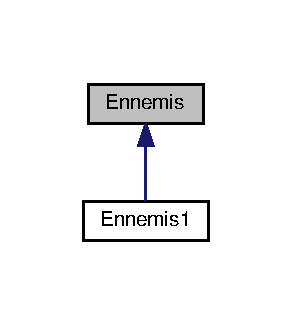
\includegraphics[width=140pt]{classEnnemis__inherit__graph}
\end{center}
\end{figure}


Graphe de collaboration de Ennemis\+:\nopagebreak
\begin{figure}[H]
\begin{center}
\leavevmode
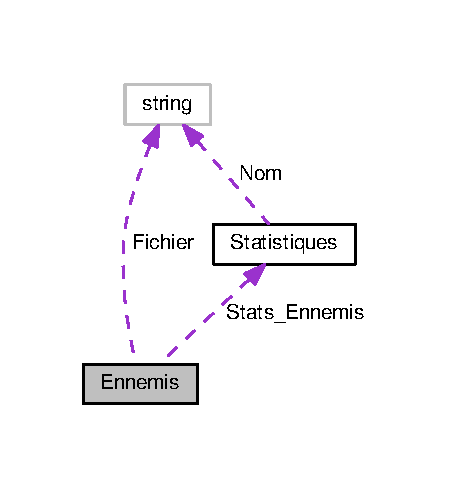
\includegraphics[width=216pt]{classEnnemis__coll__graph}
\end{center}
\end{figure}
\subsection*{Fonctions membres publiques}
\begin{DoxyCompactItemize}
\item 
\hypertarget{classEnnemis_a7808509ce0936d2d0bfe865be457edb3}{\hyperlink{classEnnemis_a7808509ce0936d2d0bfe865be457edb3}{Ennemis} ()}\label{classEnnemis_a7808509ce0936d2d0bfe865be457edb3}

\begin{DoxyCompactList}\small\item\em Initialise l'ennemi tout a 0 sauf le nom \char`\"{} \char`\"{}. \end{DoxyCompactList}\item 
\hypertarget{classEnnemis_a3496a4049af3228262235819566b2891}{\hyperlink{classEnnemis_a3496a4049af3228262235819566b2891}{Ennemis} (unsigned int x\+\_\+mini\+\_\+carte, unsigned int y\+\_\+\+Mini\+\_\+carte, char direction, char direction\+\_\+attaque, class \hyperlink{classStatistiques}{Statistiques} stats)}\label{classEnnemis_a3496a4049af3228262235819566b2891}

\begin{DoxyCompactList}\small\item\em Initialise l'ennemi par les donn�es. \end{DoxyCompactList}\item 
virtual \hyperlink{classEnnemis_abdd55d6682308cc9c7c6deb6333f215d}{$\sim$\+Ennemis} ()
\item 
\hypertarget{classEnnemis_ae89be698a072c46e884fb70f14130f4c}{const unsigned int \hyperlink{classEnnemis_ae89be698a072c46e884fb70f14130f4c}{get\+\_\+\+Position\+\_\+\+X\+\_\+\+Mini\+\_\+\+Carte} () const }\label{classEnnemis_ae89be698a072c46e884fb70f14130f4c}

\begin{DoxyCompactList}\small\item\em Renvoie la position horizontal de l'ennemi sur la mini-\/carte. \end{DoxyCompactList}\item 
\hypertarget{classEnnemis_a1a20a88b268a105ea1d21980e9be2a29}{const unsigned int \hyperlink{classEnnemis_a1a20a88b268a105ea1d21980e9be2a29}{get\+\_\+\+Position\+\_\+\+Y\+\_\+\+Mini\+\_\+\+Carte} () const }\label{classEnnemis_a1a20a88b268a105ea1d21980e9be2a29}

\begin{DoxyCompactList}\small\item\em Renvoie la position verticale de l'ennemi sur la mini-\/carte. \end{DoxyCompactList}\item 
\hypertarget{classEnnemis_a7a685ab62b81f994284864c4f6e0ac1d}{const char \hyperlink{classEnnemis_a7a685ab62b81f994284864c4f6e0ac1d}{get\+\_\+\+Direction} () const }\label{classEnnemis_a7a685ab62b81f994284864c4f6e0ac1d}

\begin{DoxyCompactList}\small\item\em Renvoie la direction de l'ennemi. \end{DoxyCompactList}\item 
\hypertarget{classEnnemis_a727873d26be409882ca80c897e584d2b}{const char \hyperlink{classEnnemis_a727873d26be409882ca80c897e584d2b}{get\+\_\+\+Direction\+\_\+\+Attaque} () const }\label{classEnnemis_a727873d26be409882ca80c897e584d2b}

\begin{DoxyCompactList}\small\item\em Renvoie la valeur de la direction de l'attaque. \end{DoxyCompactList}\item 
\hypertarget{classEnnemis_a0b2b108d20ac8d7c18a7a1a72965f8ef}{const class \hyperlink{classStatistiques}{Statistiques} \hyperlink{classEnnemis_a0b2b108d20ac8d7c18a7a1a72965f8ef}{get\+\_\+\+Stats\+\_\+\+Ennemis} () const }\label{classEnnemis_a0b2b108d20ac8d7c18a7a1a72965f8ef}

\begin{DoxyCompactList}\small\item\em Renvoi la mergingstatistique de l'ennemi. \end{DoxyCompactList}\item 
\hypertarget{classEnnemis_a8cfcd0524e6c6f1cdf75a13ecf6d8cd3}{const string \hyperlink{classEnnemis_a8cfcd0524e6c6f1cdf75a13ecf6d8cd3}{get\+\_\+\+Stats\+\_\+\+Ennemis\+\_\+\+Nom} () const }\label{classEnnemis_a8cfcd0524e6c6f1cdf75a13ecf6d8cd3}

\begin{DoxyCompactList}\small\item\em Retourne le nom de l'ennemi. \end{DoxyCompactList}\item 
\hypertarget{classEnnemis_a1cb88131ba57e81a6d970caeb4ff2e1c}{const unsigned int \hyperlink{classEnnemis_a1cb88131ba57e81a6d970caeb4ff2e1c}{get\+\_\+\+Stats\+\_\+\+Ennemis\+\_\+\+Point\+\_\+\+De\+\_\+\+Vie} () const }\label{classEnnemis_a1cb88131ba57e81a6d970caeb4ff2e1c}

\begin{DoxyCompactList}\small\item\em Retourne les pv de l'ennemi. \end{DoxyCompactList}\item 
\hypertarget{classEnnemis_a1b0b8b665428cab760d2502b4f073704}{const unsigned int \hyperlink{classEnnemis_a1b0b8b665428cab760d2502b4f073704}{get\+\_\+\+Stats\+\_\+\+Ennemis\+\_\+\+Point\+\_\+\+De\+\_\+\+Vie\+\_\+\+Max} () const }\label{classEnnemis_a1b0b8b665428cab760d2502b4f073704}

\begin{DoxyCompactList}\small\item\em Retourne les pv\+\_\+max de l'ennemi. \end{DoxyCompactList}\item 
\hypertarget{classEnnemis_acfba09fdbd6a60e42da08e26d29d2258}{const unsigned int \hyperlink{classEnnemis_acfba09fdbd6a60e42da08e26d29d2258}{get\+\_\+\+Stats\+\_\+\+Ennemis\+\_\+\+Mana} () const }\label{classEnnemis_acfba09fdbd6a60e42da08e26d29d2258}

\begin{DoxyCompactList}\small\item\em Retourne les mana de l'ennemi. \end{DoxyCompactList}\item 
\hypertarget{classEnnemis_a758eefe44b97fe4fc96045b1a26d8059}{const unsigned int \hyperlink{classEnnemis_a758eefe44b97fe4fc96045b1a26d8059}{get\+\_\+\+Stats\+\_\+\+Ennemis\+\_\+\+Mana\+\_\+\+Max} () const }\label{classEnnemis_a758eefe44b97fe4fc96045b1a26d8059}

\begin{DoxyCompactList}\small\item\em Retourne la Mana\+\_\+max de l'ennemi. \end{DoxyCompactList}\item 
\hypertarget{classEnnemis_a1eb216e259216252c7400e456d9f4403}{const unsigned int \hyperlink{classEnnemis_a1eb216e259216252c7400e456d9f4403}{get\+\_\+\+Stats\+\_\+\+Ennemis\+\_\+\+Experience\+\_\+\+Restant} () const }\label{classEnnemis_a1eb216e259216252c7400e456d9f4403}

\begin{DoxyCompactList}\small\item\em Retourne les pv de l'ennemi. \end{DoxyCompactList}\item 
\hypertarget{classEnnemis_a2198c73648c730bbc48b0917fbf32d18}{const unsigned int \hyperlink{classEnnemis_a2198c73648c730bbc48b0917fbf32d18}{get\+\_\+\+Stats\+\_\+\+Ennemis\+\_\+\+Experience\+\_\+\+Donne} () const }\label{classEnnemis_a2198c73648c730bbc48b0917fbf32d18}

\begin{DoxyCompactList}\small\item\em Retourne les xp\+\_\+donne de l'ennemi. \end{DoxyCompactList}\item 
\hypertarget{classEnnemis_ae92bc0ee3d238bdd8222ad9854c427e4}{const unsigned int \hyperlink{classEnnemis_ae92bc0ee3d238bdd8222ad9854c427e4}{get\+\_\+\+Stats\+\_\+\+Ennemis\+\_\+\+Niveau} () const }\label{classEnnemis_ae92bc0ee3d238bdd8222ad9854c427e4}

\begin{DoxyCompactList}\small\item\em Retourne le niveau de l'ennemi. \end{DoxyCompactList}\item 
\hypertarget{classEnnemis_a4faa8133b82b6b224e2549bb4e524945}{const unsigned int \hyperlink{classEnnemis_a4faa8133b82b6b224e2549bb4e524945}{get\+\_\+\+Stats\+\_\+\+Ennemis\+\_\+\+Force} () const }\label{classEnnemis_a4faa8133b82b6b224e2549bb4e524945}

\begin{DoxyCompactList}\small\item\em Retourne les forces de l'ennemi. \end{DoxyCompactList}\item 
\hypertarget{classEnnemis_a87b83871f515c3713509559bccf22af9}{const unsigned int \hyperlink{classEnnemis_a87b83871f515c3713509559bccf22af9}{get\+\_\+\+Stats\+\_\+\+Ennemis\+\_\+\+Intelligence} () const }\label{classEnnemis_a87b83871f515c3713509559bccf22af9}

\begin{DoxyCompactList}\small\item\em Retourne l'intelligence de l'ennemi. \end{DoxyCompactList}\item 
\hypertarget{classEnnemis_ab07f2f10c915a06a842e137875e07c08}{const unsigned int \hyperlink{classEnnemis_ab07f2f10c915a06a842e137875e07c08}{get\+\_\+\+Stats\+\_\+\+Ennemis\+\_\+\+Agilite} () const }\label{classEnnemis_ab07f2f10c915a06a842e137875e07c08}

\begin{DoxyCompactList}\small\item\em Retourne l'agilite de l'ennemi. \end{DoxyCompactList}\item 
\hypertarget{classEnnemis_a2facae0521547d95df12d2647285f6fc}{const string \hyperlink{classEnnemis_a2facae0521547d95df12d2647285f6fc}{get\+\_\+\+Fichier} () const }\label{classEnnemis_a2facae0521547d95df12d2647285f6fc}

\begin{DoxyCompactList}\small\item\em Retourne l'emplacement du fichier. \end{DoxyCompactList}\item 
\hypertarget{classEnnemis_aed675cd030cb462f467f3c68a041706c}{void \hyperlink{classEnnemis_aed675cd030cb462f467f3c68a041706c}{set\+\_\+\+Position\+\_\+\+X\+\_\+\+Mini\+\_\+\+Carte} (unsigned int x)}\label{classEnnemis_aed675cd030cb462f467f3c68a041706c}

\begin{DoxyCompactList}\small\item\em Acc�de � la position horizontale de l'ennemi sur la mini-\/carte. \end{DoxyCompactList}\item 
\hypertarget{classEnnemis_a94c1c1edc21e37cf07b7876aad52ffb1}{void \hyperlink{classEnnemis_a94c1c1edc21e37cf07b7876aad52ffb1}{set\+\_\+\+Position\+\_\+\+Y\+\_\+\+Mini\+\_\+\+Carte} (unsigned int y)}\label{classEnnemis_a94c1c1edc21e37cf07b7876aad52ffb1}

\begin{DoxyCompactList}\small\item\em Acc�de � la position verticale de l'ennemi sur la minicarte. \end{DoxyCompactList}\item 
\hypertarget{classEnnemis_a0146fe9c16c509235665c3577db8bd23}{void \hyperlink{classEnnemis_a0146fe9c16c509235665c3577db8bd23}{set\+\_\+\+Direction} (char direction)}\label{classEnnemis_a0146fe9c16c509235665c3577db8bd23}

\begin{DoxyCompactList}\small\item\em Acc�de � la direction de l'ennemi. \end{DoxyCompactList}\item 
\hypertarget{classEnnemis_a5c9badeeb3cce1dbb5eb56785737b88f}{void \hyperlink{classEnnemis_a5c9badeeb3cce1dbb5eb56785737b88f}{set\+\_\+\+Direction\+\_\+\+Attaque} (char direction)}\label{classEnnemis_a5c9badeeb3cce1dbb5eb56785737b88f}

\begin{DoxyCompactList}\small\item\em Modifie la valeur de la direction de l'attaque. \end{DoxyCompactList}\item 
\hypertarget{classEnnemis_a04a5da853b550ce1112f6c2c4907771e}{void \hyperlink{classEnnemis_a04a5da853b550ce1112f6c2c4907771e}{set\+\_\+\+Stats\+\_\+\+Ennemis} (class \hyperlink{classStatistiques}{Statistiques} s)}\label{classEnnemis_a04a5da853b550ce1112f6c2c4907771e}

\begin{DoxyCompactList}\small\item\em Acc�de au donn�e de la classe statistique de l'ennemi. \end{DoxyCompactList}\item 
\hypertarget{classEnnemis_a423bde7f36520e534d3d524fc62f6556}{void \hyperlink{classEnnemis_a423bde7f36520e534d3d524fc62f6556}{set\+\_\+\+Ennemis} (class \hyperlink{classEnnemis}{Ennemis} ennemis)}\label{classEnnemis_a423bde7f36520e534d3d524fc62f6556}

\begin{DoxyCompactList}\small\item\em Copie compl�tement l'ennemi en parametre (copie profonde) \end{DoxyCompactList}\item 
\hypertarget{classEnnemis_ad61b390d593d7a7db1c2778d575e112e}{void \hyperlink{classEnnemis_ad61b390d593d7a7db1c2778d575e112e}{set\+\_\+\+Ennemis} (string nom\+\_\+fichier)}\label{classEnnemis_ad61b390d593d7a7db1c2778d575e112e}

\begin{DoxyCompactList}\small\item\em Charge le fichier pour remplir les caracteristique de ennemis. \end{DoxyCompactList}\item 
\hypertarget{classEnnemis_ab1b09d47d8af999814c9a196084045c8}{void \hyperlink{classEnnemis_ab1b09d47d8af999814c9a196084045c8}{set\+\_\+\+Ennemis\+\_\+\+Fichier} ()}\label{classEnnemis_ab1b09d47d8af999814c9a196084045c8}

\begin{DoxyCompactList}\small\item\em Charge uniquement le fichier dans les donn�e corespondants. \end{DoxyCompactList}\item 
\hypertarget{classEnnemis_a935d4f7ad6314dd755c993ba6b42fd2f}{void \hyperlink{classEnnemis_a935d4f7ad6314dd755c993ba6b42fd2f}{set\+\_\+\+Fichier} (string nom\+\_\+fichier)}\label{classEnnemis_a935d4f7ad6314dd755c993ba6b42fd2f}

\begin{DoxyCompactList}\small\item\em remplie le nom du fichier \end{DoxyCompactList}\item 
\hypertarget{classEnnemis_ae37fb4d0bd301483e65fa7f38bcb7771}{void \hyperlink{classEnnemis_ae37fb4d0bd301483e65fa7f38bcb7771}{set\+\_\+\+Stats\+\_\+\+Ennemis\+\_\+\+Nom} (string nom)}\label{classEnnemis_ae37fb4d0bd301483e65fa7f38bcb7771}

\begin{DoxyCompactList}\small\item\em Modifie le nom de l'ennemi. \end{DoxyCompactList}\item 
\hypertarget{classEnnemis_aa718e897cf74834a59c1664349bf46e9}{void \hyperlink{classEnnemis_aa718e897cf74834a59c1664349bf46e9}{set\+\_\+\+Stats\+\_\+\+Ennemis\+\_\+\+Point\+\_\+\+De\+\_\+\+Vie} (unsigned int pv)}\label{classEnnemis_aa718e897cf74834a59c1664349bf46e9}

\begin{DoxyCompactList}\small\item\em Modifie les pv de l'ennemi. \end{DoxyCompactList}\item 
\hypertarget{classEnnemis_ae7800953b257fb5c0294cb05866624a8}{void \hyperlink{classEnnemis_ae7800953b257fb5c0294cb05866624a8}{set\+\_\+\+Stats\+\_\+\+Ennemis\+\_\+\+Point\+\_\+\+De\+\_\+\+Vie\+\_\+\+Max} (unsigned int pv\+\_\+max)}\label{classEnnemis_ae7800953b257fb5c0294cb05866624a8}

\begin{DoxyCompactList}\small\item\em Modifie les pv\+\_\+max de l'ennemi. \end{DoxyCompactList}\item 
\hypertarget{classEnnemis_ac29470e84f642c904096d9676a5ed395}{void \hyperlink{classEnnemis_ac29470e84f642c904096d9676a5ed395}{set\+\_\+\+Stats\+\_\+\+Ennemis\+\_\+\+Mana} (unsigned int mana)}\label{classEnnemis_ac29470e84f642c904096d9676a5ed395}

\begin{DoxyCompactList}\small\item\em Modifie les mana de l'ennemi. \end{DoxyCompactList}\item 
\hypertarget{classEnnemis_a495ecb459e28e648d572415e1ec5aa25}{void \hyperlink{classEnnemis_a495ecb459e28e648d572415e1ec5aa25}{set\+\_\+\+Stats\+\_\+\+Ennemis\+\_\+\+Mana\+\_\+\+Max} (unsigned int mana\+\_\+max)}\label{classEnnemis_a495ecb459e28e648d572415e1ec5aa25}

\begin{DoxyCompactList}\small\item\em Modifie la Mana\+\_\+max de l'ennemi. \end{DoxyCompactList}\item 
\hypertarget{classEnnemis_afa83775bbada9f74e65661b390191681}{void \hyperlink{classEnnemis_afa83775bbada9f74e65661b390191681}{set\+\_\+\+Stats\+\_\+\+Ennemis\+\_\+\+Experience\+\_\+\+Restant} (unsigned int xp\+\_\+restant)}\label{classEnnemis_afa83775bbada9f74e65661b390191681}

\begin{DoxyCompactList}\small\item\em Modifie les xp restants pour le prochain niveau de l'ennemi. \end{DoxyCompactList}\item 
\hypertarget{classEnnemis_a27f9f592a4b421f8462ba7dac26203f3}{void \hyperlink{classEnnemis_a27f9f592a4b421f8462ba7dac26203f3}{set\+\_\+\+Stats\+\_\+\+Ennemis\+\_\+\+Experience\+\_\+\+Donne} (unsigned int xp\+\_\+donne)}\label{classEnnemis_a27f9f592a4b421f8462ba7dac26203f3}

\begin{DoxyCompactList}\small\item\em Modifie les xp\+\_\+donne de l'ennemi. \end{DoxyCompactList}\item 
\hypertarget{classEnnemis_a00d4a5f41c7aa3226dd046583a9a034c}{void \hyperlink{classEnnemis_a00d4a5f41c7aa3226dd046583a9a034c}{set\+\_\+\+Stats\+\_\+\+Ennemis\+\_\+\+Niveau} (unsigned int niv)}\label{classEnnemis_a00d4a5f41c7aa3226dd046583a9a034c}

\begin{DoxyCompactList}\small\item\em Modifie le niveau de l'ennemi. \end{DoxyCompactList}\item 
\hypertarget{classEnnemis_a3021a2d2b89a692cd82d6bd2cc771cb4}{void \hyperlink{classEnnemis_a3021a2d2b89a692cd82d6bd2cc771cb4}{set\+\_\+\+Stats\+\_\+\+Ennemis\+\_\+\+Force} (unsigned int force)}\label{classEnnemis_a3021a2d2b89a692cd82d6bd2cc771cb4}

\begin{DoxyCompactList}\small\item\em Modifie les forces de l'ennemi. \end{DoxyCompactList}\item 
\hypertarget{classEnnemis_acc87b692aadaabd9bbb217e9a34fb75a}{void \hyperlink{classEnnemis_acc87b692aadaabd9bbb217e9a34fb75a}{set\+\_\+\+Stats\+\_\+\+Ennemis\+\_\+\+Intelligence} (unsigned int intelligence)}\label{classEnnemis_acc87b692aadaabd9bbb217e9a34fb75a}

\begin{DoxyCompactList}\small\item\em Modifie l'intelligence de l'ennemi. \end{DoxyCompactList}\item 
\hypertarget{classEnnemis_a9114dc9c39e984ea18c5243b8da6b4e6}{void \hyperlink{classEnnemis_a9114dc9c39e984ea18c5243b8da6b4e6}{set\+\_\+\+Stats\+\_\+\+Ennemis\+\_\+\+Agilite} (unsigned int agilite)}\label{classEnnemis_a9114dc9c39e984ea18c5243b8da6b4e6}

\begin{DoxyCompactList}\small\item\em Modifie l'agilite de l'ennemi. \end{DoxyCompactList}\item 
\hypertarget{classEnnemis_aed3349489e4fd823edee09babce3a301}{void \hyperlink{classEnnemis_aed3349489e4fd823edee09babce3a301}{Deplacement\+\_\+\+Ennemis\+\_\+\+Automatique} (class \hyperlink{classMini__Carte}{Mini\+\_\+\+Carte} \&mini\+\_\+carte)}\label{classEnnemis_aed3349489e4fd823edee09babce3a301}

\begin{DoxyCompactList}\small\item\em Fait bouger le monstre. \end{DoxyCompactList}\item 
\hypertarget{classEnnemis_aca2a24530ae2cffca145e7f258415301}{void \hyperlink{classEnnemis_aca2a24530ae2cffca145e7f258415301}{Deplacement\+\_\+\+Ennemis\+\_\+\+Script} (const class \hyperlink{classMini__Carte}{Mini\+\_\+\+Carte} \&mini\+\_\+carte)}\label{classEnnemis_aca2a24530ae2cffca145e7f258415301}

\begin{DoxyCompactList}\small\item\em Fait bouger l'ennemi selon un script. \end{DoxyCompactList}\item 
\hypertarget{classEnnemis_ac02d4bc708888d4f7710d07afeb64cdf}{\hyperlink{classObjet}{Objet} \hyperlink{classEnnemis_ac02d4bc708888d4f7710d07afeb64cdf}{Lache\+\_\+\+Objet} (\hyperlink{classObjet}{Objet} objet)}\label{classEnnemis_ac02d4bc708888d4f7710d07afeb64cdf}

\begin{DoxyCompactList}\small\item\em Peut renvoyer un objet quand il meurt. \end{DoxyCompactList}\item 
\hypertarget{classEnnemis_ad93c569453b7127c1364f4b8488f0c0b}{bool \hyperlink{classEnnemis_ad93c569453b7127c1364f4b8488f0c0b}{Heros\+\_\+\+Visible\+\_\+\+Par\+\_\+\+Ennemis} (unsigned int Position\+\_\+\+Heros\+\_\+\+X, unsigned int Position\+\_\+\+Heros\+\_\+\+Y)}\label{classEnnemis_ad93c569453b7127c1364f4b8488f0c0b}

\begin{DoxyCompactList}\small\item\em Renvoie true si heros est dans le champ de vision de l'ennemis prend l'agrro ou pas. \end{DoxyCompactList}\item 
\hypertarget{classEnnemis_aeaf1fe3792f5ab7ea712205651f96ecb}{unsigned int \hyperlink{classEnnemis_aeaf1fe3792f5ab7ea712205651f96ecb}{Attaque\+\_\+\+Ennemis} (const \hyperlink{classMini__Carte}{Mini\+\_\+\+Carte} \&mini\+\_\+carte)}\label{classEnnemis_aeaf1fe3792f5ab7ea712205651f96ecb}

\begin{DoxyCompactList}\small\item\em Attaque ennemis en fonction de sa capacit� � attaquer diagonale laterale horizontale ... \end{DoxyCompactList}\item 
\hypertarget{classEnnemis_af535d5bfebc82874e281436000942286}{void \hyperlink{classEnnemis_af535d5bfebc82874e281436000942286}{Affiche\+\_\+\+Ennemis} () const }\label{classEnnemis_af535d5bfebc82874e281436000942286}

\begin{DoxyCompactList}\small\item\em Affiche toutes les donn�es membres. \end{DoxyCompactList}\item 
\hypertarget{classEnnemis_a329aaf9b835aa3d222b52ea857c7daf7}{bool \hyperlink{classEnnemis_a329aaf9b835aa3d222b52ea857c7daf7}{Ennemis\+\_\+\+Touche} (unsigned int x, unsigned int y)}\label{classEnnemis_a329aaf9b835aa3d222b52ea857c7daf7}

\begin{DoxyCompactList}\small\item\em renvoie si l'ennemi est toucher \end{DoxyCompactList}\item 
\hypertarget{classEnnemis_ad150d68159d55ce1c581d5ed651c9194}{void \hyperlink{classEnnemis_ad150d68159d55ce1c581d5ed651c9194}{Ennemis\+\_\+\+Touche} (unsigned int degats)}\label{classEnnemis_ad150d68159d55ce1c581d5ed651c9194}

\begin{DoxyCompactList}\small\item\em modifie les points de vie de l'attaque \end{DoxyCompactList}\item 
\hypertarget{classEnnemis_a9b612546a4b417be077775b75b8c97df}{void \hyperlink{classEnnemis_a9b612546a4b417be077775b75b8c97df}{Test\+\_\+\+Regression} ()}\label{classEnnemis_a9b612546a4b417be077775b75b8c97df}

\begin{DoxyCompactList}\small\item\em V�rifie toutes les fonctions. \end{DoxyCompactList}\item 
\hypertarget{classEnnemis_aced9e77803e38857f2d185ceca251dda}{bool \hyperlink{classEnnemis_aced9e77803e38857f2d185ceca251dda}{Toucher\+\_\+\+Heros} (unsigned int position\+\_\+x, unsigned int position\+\_\+y, unsigned int position\+\_\+heros\+\_\+x, unsigned int position\+\_\+heros\+\_\+y)}\label{classEnnemis_aced9e77803e38857f2d185ceca251dda}

\begin{DoxyCompactList}\small\item\em Verifie attaque touche heros. \end{DoxyCompactList}\item 
\hypertarget{classEnnemis_a94014214d19187985d3b76ba20474cd3}{bool \hyperlink{classEnnemis_a94014214d19187985d3b76ba20474cd3}{Ennemis\+\_\+\+Mort} ()}\label{classEnnemis_a94014214d19187985d3b76ba20474cd3}

\begin{DoxyCompactList}\small\item\em verifie si ennemis mort ou pas \end{DoxyCompactList}\end{DoxyCompactItemize}
\subsection*{Attributs privés}
\begin{DoxyCompactItemize}
\item 
\hypertarget{classEnnemis_ad3858f14191b00287b17ccb6a9a34e72}{unsigned int \hyperlink{classEnnemis_ad3858f14191b00287b17ccb6a9a34e72}{Position\+\_\+\+X\+\_\+\+Mini\+\_\+\+Carte}}\label{classEnnemis_ad3858f14191b00287b17ccb6a9a34e72}

\begin{DoxyCompactList}\small\item\em Position horizontale de l'ennemi sur la Mini-\/carte. \end{DoxyCompactList}\item 
\hypertarget{classEnnemis_a278ade60950826808bb6a2b5b0b265d5}{unsigned int \hyperlink{classEnnemis_a278ade60950826808bb6a2b5b0b265d5}{Position\+\_\+\+Y\+\_\+\+Mini\+\_\+\+Carte}}\label{classEnnemis_a278ade60950826808bb6a2b5b0b265d5}

\begin{DoxyCompactList}\small\item\em Position verticale de l'ennemi sur la Mini-\/carte. \end{DoxyCompactList}\item 
\hypertarget{classEnnemis_ae7c6f94311950316d3f50fe12d4fa9ee}{char \hyperlink{classEnnemis_ae7c6f94311950316d3f50fe12d4fa9ee}{Direction}}\label{classEnnemis_ae7c6f94311950316d3f50fe12d4fa9ee}

\begin{DoxyCompactList}\small\item\em Direction de l'ennemis. \end{DoxyCompactList}\item 
\hypertarget{classEnnemis_aec6ec2d257ca821acadc0275344f6d0c}{char \hyperlink{classEnnemis_aec6ec2d257ca821acadc0275344f6d0c}{Direction\+\_\+\+Attaque}}\label{classEnnemis_aec6ec2d257ca821acadc0275344f6d0c}

\begin{DoxyCompactList}\small\item\em Donne la direction de l'attaque h=horizontal, l=lateral,d= diagonal. \end{DoxyCompactList}\item 
\hypertarget{classEnnemis_a00247b374148e02ec6ca550354d74eb0}{\hyperlink{classStatistiques}{Statistiques} \hyperlink{classEnnemis_a00247b374148e02ec6ca550354d74eb0}{Stats\+\_\+\+Ennemis}}\label{classEnnemis_a00247b374148e02ec6ca550354d74eb0}

\begin{DoxyCompactList}\small\item\em \hyperlink{classStatistiques}{Statistiques} de l'ennemi. \end{DoxyCompactList}\item 
\hypertarget{classEnnemis_a4f82e81c2993d0dcd1d2178cdc7a1b39}{string \hyperlink{classEnnemis_a4f82e81c2993d0dcd1d2178cdc7a1b39}{Fichier}}\label{classEnnemis_a4f82e81c2993d0dcd1d2178cdc7a1b39}

\begin{DoxyCompactList}\small\item\em Le fichier qui contient les statistiques, la Direction,la direction de l'attaque. \end{DoxyCompactList}\end{DoxyCompactItemize}


\subsection{Documentation des constructeurs et destructeur}
\hypertarget{classEnnemis_abdd55d6682308cc9c7c6deb6333f215d}{\index{Ennemis@{Ennemis}!````~Ennemis@{$\sim$\+Ennemis}}
\index{````~Ennemis@{$\sim$\+Ennemis}!Ennemis@{Ennemis}}
\subsubsection[{$\sim$\+Ennemis}]{\setlength{\rightskip}{0pt plus 5cm}Ennemis\+::$\sim$\+Ennemis (
\begin{DoxyParamCaption}
{}
\end{DoxyParamCaption}
)\hspace{0.3cm}{\ttfamily [virtual]}}}\label{classEnnemis_abdd55d6682308cc9c7c6deb6333f215d}
Default Destructeur 

La documentation de cette classe a été générée à partir des fichiers suivants \+:\begin{DoxyCompactItemize}
\item 
src/include/Ennemis.\+h\item 
src/cpp/Ennemis.\+cpp\end{DoxyCompactItemize}

\hypertarget{classEnnemis1}{\section{Référence de la classe Ennemis1}
\label{classEnnemis1}\index{Ennemis1@{Ennemis1}}
}


Graphe d'héritage de Ennemis1\+:\nopagebreak
\begin{figure}[H]
\begin{center}
\leavevmode
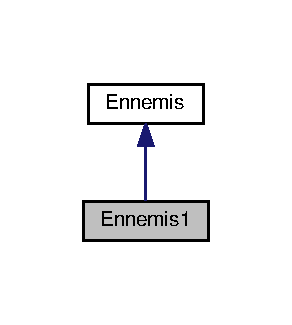
\includegraphics[width=140pt]{classEnnemis1__inherit__graph}
\end{center}
\end{figure}


Graphe de collaboration de Ennemis1\+:\nopagebreak
\begin{figure}[H]
\begin{center}
\leavevmode
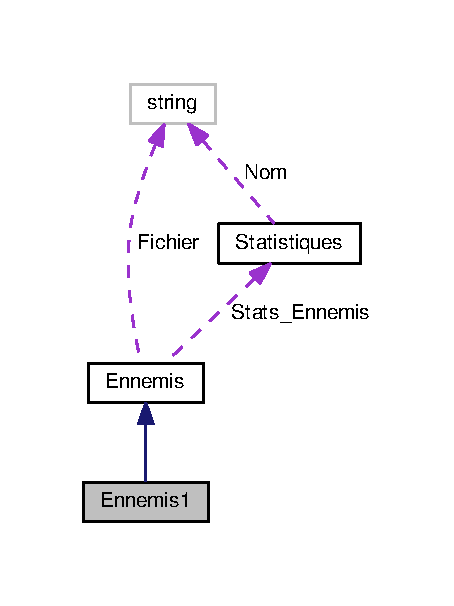
\includegraphics[width=218pt]{classEnnemis1__coll__graph}
\end{center}
\end{figure}
\subsection*{Classes}
\begin{DoxyCompactItemize}
\item 
class \hyperlink{classEnnemis1_1_1h}{h}
\end{DoxyCompactItemize}
\subsection*{Fonctions membres publiques}
\begin{DoxyCompactItemize}
\item 
\hyperlink{classEnnemis1_a0a982d19052c62902ef0ef9e255fb02a}{Ennemis1} ()
\item 
virtual \hyperlink{classEnnemis1_ab3a6b6e19a786968264235af0beef8e3}{$\sim$\+Ennemis1} ()
\end{DoxyCompactItemize}


\subsection{Documentation des constructeurs et destructeur}
\hypertarget{classEnnemis1_a0a982d19052c62902ef0ef9e255fb02a}{\index{Ennemis1@{Ennemis1}!Ennemis1@{Ennemis1}}
\index{Ennemis1@{Ennemis1}!Ennemis1@{Ennemis1}}
\subsubsection[{Ennemis1}]{\setlength{\rightskip}{0pt plus 5cm}Ennemis1\+::\+Ennemis1 (
\begin{DoxyParamCaption}
{}
\end{DoxyParamCaption}
)}}\label{classEnnemis1_a0a982d19052c62902ef0ef9e255fb02a}
Default constructor \hypertarget{classEnnemis1_ab3a6b6e19a786968264235af0beef8e3}{\index{Ennemis1@{Ennemis1}!````~Ennemis1@{$\sim$\+Ennemis1}}
\index{````~Ennemis1@{$\sim$\+Ennemis1}!Ennemis1@{Ennemis1}}
\subsubsection[{$\sim$\+Ennemis1}]{\setlength{\rightskip}{0pt plus 5cm}virtual Ennemis1\+::$\sim$\+Ennemis1 (
\begin{DoxyParamCaption}
{}
\end{DoxyParamCaption}
)\hspace{0.3cm}{\ttfamily [virtual]}}}\label{classEnnemis1_ab3a6b6e19a786968264235af0beef8e3}
Default destructor 

La documentation de cette classe a été générée à partir du fichier suivant \+:\begin{DoxyCompactItemize}
\item 
src/include/Ennemis1.\+h\end{DoxyCompactItemize}

\hypertarget{classEquipement}{\section{Référence de la classe Equipement}
\label{classEquipement}\index{Equipement@{Equipement}}
}


Graphe de collaboration de Equipement\+:\nopagebreak
\begin{figure}[H]
\begin{center}
\leavevmode
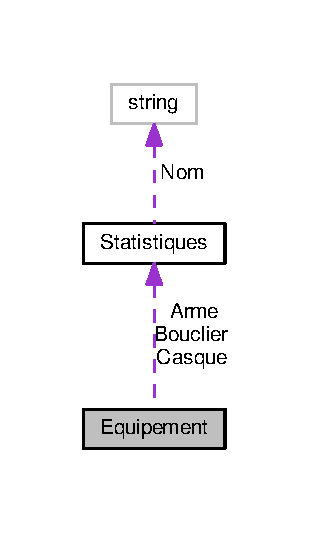
\includegraphics[width=150pt]{classEquipement__coll__graph}
\end{center}
\end{figure}
\subsection*{Fonctions membres publiques}
\begin{DoxyCompactItemize}
\item 
\hypertarget{classEquipement_a9057a4777d006cbac4c72d09a8d09407}{\hyperlink{classEquipement_a9057a4777d006cbac4c72d09a8d09407}{Equipement} ()}\label{classEquipement_a9057a4777d006cbac4c72d09a8d09407}

\begin{DoxyCompactList}\small\item\em Constructeur. \end{DoxyCompactList}\item 
\hyperlink{classEquipement_ae7751a52f2665d9e4b3e2cd6929bd986}{$\sim$\+Equipement} ()
\begin{DoxyCompactList}\small\item\em Destructeur. \end{DoxyCompactList}\item 
\hypertarget{classEquipement_ab2c04a8c70fadc1372b56bd9612ac56e}{class \hyperlink{classStatistiques}{Statistiques} \hyperlink{classEquipement_ab2c04a8c70fadc1372b56bd9612ac56e}{get\+\_\+\+Stats\+\_\+\+Arme} () const }\label{classEquipement_ab2c04a8c70fadc1372b56bd9612ac56e}

\begin{DoxyCompactList}\small\item\em Retourne les statistiques de l'arme. \end{DoxyCompactList}\item 
\hypertarget{classEquipement_a0222c5cf1ff2251126da26ad678ebdb9}{class \hyperlink{classStatistiques}{Statistiques} \hyperlink{classEquipement_a0222c5cf1ff2251126da26ad678ebdb9}{get\+\_\+\+Stats\+\_\+\+Bouclier} () const }\label{classEquipement_a0222c5cf1ff2251126da26ad678ebdb9}

\begin{DoxyCompactList}\small\item\em Retourne les statistiques du bouclier. \end{DoxyCompactList}\item 
\hypertarget{classEquipement_aae0c95310f5e628067e7341de9d461d5}{class \hyperlink{classStatistiques}{Statistiques} \hyperlink{classEquipement_aae0c95310f5e628067e7341de9d461d5}{get\+\_\+\+Stats\+\_\+\+Casque} () const }\label{classEquipement_aae0c95310f5e628067e7341de9d461d5}

\begin{DoxyCompactList}\small\item\em Retourne les statistiques du casque. \end{DoxyCompactList}\item 
\hypertarget{classEquipement_a055d306ee5f124d8681774d308b3837f}{void \hyperlink{classEquipement_a055d306ee5f124d8681774d308b3837f}{set\+\_\+\+Stats\+\_\+\+Arme} (class \hyperlink{classStatistiques}{Statistiques} Arme\+\_\+nouv)}\label{classEquipement_a055d306ee5f124d8681774d308b3837f}

\begin{DoxyCompactList}\small\item\em Modifie les staistiques de l'arme. \end{DoxyCompactList}\item 
\hypertarget{classEquipement_a5a6e71f45a0e21083394069f2e4cdfb6}{void \hyperlink{classEquipement_a5a6e71f45a0e21083394069f2e4cdfb6}{set\+\_\+\+Stats\+\_\+\+Bouclier} (class \hyperlink{classStatistiques}{Statistiques} Bouclier\+\_\+nouv)}\label{classEquipement_a5a6e71f45a0e21083394069f2e4cdfb6}

\begin{DoxyCompactList}\small\item\em Modifie les staistiques du bouclier. \end{DoxyCompactList}\item 
\hypertarget{classEquipement_adfef6a87d15d5186622ca3deff7b0d72}{void \hyperlink{classEquipement_adfef6a87d15d5186622ca3deff7b0d72}{set\+\_\+\+Stats\+\_\+\+Casque} (class \hyperlink{classStatistiques}{Statistiques} Casque\+\_\+nouv)}\label{classEquipement_adfef6a87d15d5186622ca3deff7b0d72}

\begin{DoxyCompactList}\small\item\em Modifie les staistiques du casque. \end{DoxyCompactList}\item 
\hypertarget{classEquipement_a14dcc7f2c37b5fec5d21cbe974651b39}{void \hyperlink{classEquipement_a14dcc7f2c37b5fec5d21cbe974651b39}{Test\+\_\+\+Regression} ()}\label{classEquipement_a14dcc7f2c37b5fec5d21cbe974651b39}

\begin{DoxyCompactList}\small\item\em Test de r�gression de la classe. \end{DoxyCompactList}\end{DoxyCompactItemize}
\subsection*{Attributs privés}
\begin{DoxyCompactItemize}
\item 
\hypertarget{classEquipement_a2fe79e8dd45074604a2f854bd095df11}{\hyperlink{classStatistiques}{Statistiques} \hyperlink{classEquipement_a2fe79e8dd45074604a2f854bd095df11}{Arme}}\label{classEquipement_a2fe79e8dd45074604a2f854bd095df11}

\begin{DoxyCompactList}\small\item\em Caract�ristiques de l'arme du personnage. \end{DoxyCompactList}\item 
\hypertarget{classEquipement_a12b0d38f18099ee1c58d151ccfa09723}{\hyperlink{classStatistiques}{Statistiques} \hyperlink{classEquipement_a12b0d38f18099ee1c58d151ccfa09723}{Bouclier}}\label{classEquipement_a12b0d38f18099ee1c58d151ccfa09723}

\begin{DoxyCompactList}\small\item\em Caract�ristiques du bouclier du personnage. \end{DoxyCompactList}\item 
\hypertarget{classEquipement_acdbcfe7d2d196d5fbcabc69926e031ed}{\hyperlink{classStatistiques}{Statistiques} \hyperlink{classEquipement_acdbcfe7d2d196d5fbcabc69926e031ed}{Casque}}\label{classEquipement_acdbcfe7d2d196d5fbcabc69926e031ed}

\begin{DoxyCompactList}\small\item\em Caract�ristiques du casque du personnage. \end{DoxyCompactList}\end{DoxyCompactItemize}


\subsection{Documentation des constructeurs et destructeur}
\hypertarget{classEquipement_ae7751a52f2665d9e4b3e2cd6929bd986}{\index{Equipement@{Equipement}!````~Equipement@{$\sim$\+Equipement}}
\index{````~Equipement@{$\sim$\+Equipement}!Equipement@{Equipement}}
\subsubsection[{$\sim$\+Equipement}]{\setlength{\rightskip}{0pt plus 5cm}Equipement\+::$\sim$\+Equipement (
\begin{DoxyParamCaption}
{}
\end{DoxyParamCaption}
)}}\label{classEquipement_ae7751a52f2665d9e4b3e2cd6929bd986}


Destructeur. 


\begin{DoxyItemize}
\item 
\end{DoxyItemize}

La documentation de cette classe a été générée à partir des fichiers suivants \+:\begin{DoxyCompactItemize}
\item 
src/include/Equipement.\+h\item 
src/cpp/Equipement.\+cpp\end{DoxyCompactItemize}

\hypertarget{classEnnemis1_1_1h}{\section{Référence de la classe Ennemis1\+:\+:h}
\label{classEnnemis1_1_1h}\index{Ennemis1\+::h@{Ennemis1\+::h}}
}


Graphe d'héritage de Ennemis1\+:\+:h\+:\nopagebreak
\begin{figure}[H]
\begin{center}
\leavevmode
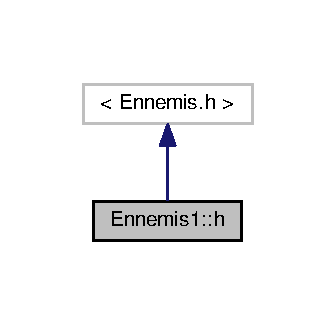
\includegraphics[width=161pt]{classEnnemis1_1_1h__inherit__graph}
\end{center}
\end{figure}


Graphe de collaboration de Ennemis1\+:\+:h\+:\nopagebreak
\begin{figure}[H]
\begin{center}
\leavevmode
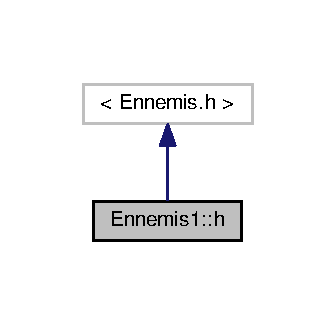
\includegraphics[width=161pt]{classEnnemis1_1_1h__coll__graph}
\end{center}
\end{figure}
\subsection*{Fonctions membres publiques}
\begin{DoxyCompactItemize}
\item 
\hyperlink{classEnnemis1}{Ennemis1} \hyperlink{classEnnemis1_1_1h_a989d42421089d7e502fefe817cc6988a}{h} ()
\item 
virtual $\sim$\hyperlink{classEnnemis1}{Ennemis1} \hyperlink{classEnnemis1_1_1h_ad10735be716514d037b089e51d551e5a}{h} ()
\end{DoxyCompactItemize}


\subsection{Documentation des constructeurs et destructeur}
\hypertarget{classEnnemis1_1_1h_a989d42421089d7e502fefe817cc6988a}{\index{Ennemis1\+::h@{Ennemis1\+::h}!h@{h}}
\index{h@{h}!Ennemis1\+::h@{Ennemis1\+::h}}
\subsubsection[{h}]{\setlength{\rightskip}{0pt plus 5cm}{\bf Ennemis1} Ennemis1\+::h\+::h (
\begin{DoxyParamCaption}
{}
\end{DoxyParamCaption}
)}}\label{classEnnemis1_1_1h_a989d42421089d7e502fefe817cc6988a}
Default constructor \hypertarget{classEnnemis1_1_1h_ad10735be716514d037b089e51d551e5a}{\index{Ennemis1\+::h@{Ennemis1\+::h}!h@{h}}
\index{h@{h}!Ennemis1\+::h@{Ennemis1\+::h}}
\subsubsection[{h}]{\setlength{\rightskip}{0pt plus 5cm}virtual $\sim${\bf Ennemis1} Ennemis1\+::h\+::h (
\begin{DoxyParamCaption}
{}
\end{DoxyParamCaption}
)\hspace{0.3cm}{\ttfamily [virtual]}}}\label{classEnnemis1_1_1h_ad10735be716514d037b089e51d551e5a}
Default destructor 

La documentation de cette classe a été générée à partir du fichier suivant \+:\begin{DoxyCompactItemize}
\item 
src/include/Ennemis1.\+h.\+h\end{DoxyCompactItemize}

\hypertarget{classHeros}{\section{Référence de la classe Heros}
\label{classHeros}\index{Heros@{Heros}}
}


Graphe de collaboration de Heros\+:\nopagebreak
\begin{figure}[H]
\begin{center}
\leavevmode
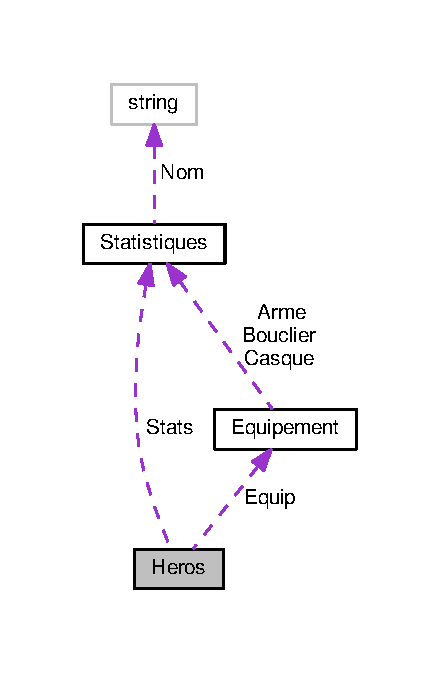
\includegraphics[width=211pt]{classHeros__coll__graph}
\end{center}
\end{figure}
\subsection*{Fonctions membres publiques}
\begin{DoxyCompactItemize}
\item 
\hypertarget{classHeros_ab4c8bc5b87a080c5f609a65bfab62c48}{\hyperlink{classHeros_ab4c8bc5b87a080c5f609a65bfab62c48}{Heros} ()}\label{classHeros_ab4c8bc5b87a080c5f609a65bfab62c48}

\begin{DoxyCompactList}\small\item\em Constructeur par d�faut. \end{DoxyCompactList}\item 
\hypertarget{classHeros_afc479810b0afa0b44b6614e75022fa61}{\hyperlink{classHeros_afc479810b0afa0b44b6614e75022fa61}{$\sim$\+Heros} ()}\label{classHeros_afc479810b0afa0b44b6614e75022fa61}

\begin{DoxyCompactList}\small\item\em Destructeur. \end{DoxyCompactList}\item 
\hypertarget{classHeros_a1ab3741f207376436bd2ed3819005c9e}{void \hyperlink{classHeros_a1ab3741f207376436bd2ed3819005c9e}{Deplace\+\_\+\+Gauche} (const class \hyperlink{classMini__Carte}{Mini\+\_\+\+Carte} \&mc)}\label{classHeros_a1ab3741f207376436bd2ed3819005c9e}

\begin{DoxyCompactList}\small\item\em D�place le h�ros vers la gauche. \end{DoxyCompactList}\item 
\hypertarget{classHeros_a1aa4518c19bdd51ef77752695cbb2520}{void \hyperlink{classHeros_a1aa4518c19bdd51ef77752695cbb2520}{Deplace\+\_\+\+Droite} (const class \hyperlink{classMini__Carte}{Mini\+\_\+\+Carte} \&mc)}\label{classHeros_a1aa4518c19bdd51ef77752695cbb2520}

\begin{DoxyCompactList}\small\item\em D�place le h�ros vers la droite. \end{DoxyCompactList}\item 
\hypertarget{classHeros_a0863f6cb0b9789cf2123ec2b41dd680e}{void \hyperlink{classHeros_a0863f6cb0b9789cf2123ec2b41dd680e}{Deplace\+\_\+\+Bas} (const class \hyperlink{classMini__Carte}{Mini\+\_\+\+Carte} \&mc)}\label{classHeros_a0863f6cb0b9789cf2123ec2b41dd680e}

\begin{DoxyCompactList}\small\item\em D�place le h�ros vers le bas. \end{DoxyCompactList}\item 
\hypertarget{classHeros_a9df03a11585acaf74ba6dbc6247a43a0}{void \hyperlink{classHeros_a9df03a11585acaf74ba6dbc6247a43a0}{Saut} (const class \hyperlink{classMini__Carte}{Mini\+\_\+\+Carte} \&mc)}\label{classHeros_a9df03a11585acaf74ba6dbc6247a43a0}

\begin{DoxyCompactList}\small\item\em D�place le h�ros vers le haut. \end{DoxyCompactList}\item 
\hypertarget{classHeros_a8852cbba7889dfa7c983f915fafe9197}{void \hyperlink{classHeros_a8852cbba7889dfa7c983f915fafe9197}{Deplace\+\_\+\+Haut} (const class \hyperlink{classMini__Carte}{Mini\+\_\+\+Carte} \&mc)}\label{classHeros_a8852cbba7889dfa7c983f915fafe9197}

\begin{DoxyCompactList}\small\item\em D�place le h�ros vers le haut. \end{DoxyCompactList}\item 
\hypertarget{classHeros_aad37d9689ae2e36dafe3490ef437fee2}{void \hyperlink{classHeros_aad37d9689ae2e36dafe3490ef437fee2}{Gravite} (const class \hyperlink{classMini__Carte}{Mini\+\_\+\+Carte} \&mc)}\label{classHeros_aad37d9689ae2e36dafe3490ef437fee2}

\begin{DoxyCompactList}\small\item\em D�place automatiquement le joueur vers le bas s'il y a du vide sous lui. \end{DoxyCompactList}\item 
\hypertarget{classHeros_acdbd5d0db9cad6a5857bd1fd5a080506}{unsigned int \hyperlink{classHeros_acdbd5d0db9cad6a5857bd1fd5a080506}{Attaque\+\_\+\+Arme} (const \hyperlink{classMini__Carte}{Mini\+\_\+\+Carte} \&mini\+\_\+carte)}\label{classHeros_acdbd5d0db9cad6a5857bd1fd5a080506}

\begin{DoxyCompactList}\small\item\em Le h�ros donne un coup d'�p�e \end{DoxyCompactList}\item 
\hypertarget{classHeros_a85c5fb4e165183d946a7c9dba57ca453}{unsigned int \hyperlink{classHeros_a85c5fb4e165183d946a7c9dba57ca453}{Attaque\+\_\+\+Magique} (const \hyperlink{classMini__Carte}{Mini\+\_\+\+Carte} \&mini\+\_\+carte, unsigned int \&posy)}\label{classHeros_a85c5fb4e165183d946a7c9dba57ca453}

\begin{DoxyCompactList}\small\item\em Le h�ros utilise une attaque magique. \end{DoxyCompactList}\item 
\hypertarget{classHeros_afdfbbbffa4b29a990f518dd1c04860de}{bool \hyperlink{classHeros_afdfbbbffa4b29a990f518dd1c04860de}{Est\+\_\+\+Sur\+\_\+\+La\+\_\+\+Meme\+\_\+\+Case\+\_\+\+Que\+\_\+\+Ennemi} (const class \hyperlink{classMini__Carte}{Mini\+\_\+\+Carte} \&mc)}\label{classHeros_afdfbbbffa4b29a990f518dd1c04860de}

\begin{DoxyCompactList}\small\item\em V�rifie si le h�ros est sur la m�me case que l'ennemi. \end{DoxyCompactList}\item 
\hypertarget{classHeros_ae9e361c189e86cb98728c0a9fd0b19a2}{unsigned int \hyperlink{classHeros_ae9e361c189e86cb98728c0a9fd0b19a2}{get\+\_\+\+Position\+\_\+\+X\+\_\+\+Mini\+\_\+\+Carte} () const }\label{classHeros_ae9e361c189e86cb98728c0a9fd0b19a2}

\begin{DoxyCompactList}\small\item\em Retourne la position horizontale du h�ros sur la mini carte. \end{DoxyCompactList}\item 
\hypertarget{classHeros_afbd9ee91886d79725f7492a86df08e48}{unsigned int \hyperlink{classHeros_afbd9ee91886d79725f7492a86df08e48}{get\+\_\+\+Position\+\_\+\+Y\+\_\+\+Mini\+\_\+\+Carte} () const }\label{classHeros_afbd9ee91886d79725f7492a86df08e48}

\begin{DoxyCompactList}\small\item\em Retourne la position verticale du h�ros sur la mini carte. \end{DoxyCompactList}\item 
\hypertarget{classHeros_a8281961057b16c040ea1a5cf1f31b444}{unsigned int \hyperlink{classHeros_a8281961057b16c040ea1a5cf1f31b444}{get\+\_\+\+Position\+\_\+\+X\+\_\+\+Carte} () const }\label{classHeros_a8281961057b16c040ea1a5cf1f31b444}

\begin{DoxyCompactList}\small\item\em Retourne la position horizontale du h�ros sur la carte. \end{DoxyCompactList}\item 
\hypertarget{classHeros_a72a9b02182178b0331375e268095287e}{unsigned int \hyperlink{classHeros_a72a9b02182178b0331375e268095287e}{get\+\_\+\+Position\+\_\+\+Y\+\_\+\+Carte} () const }\label{classHeros_a72a9b02182178b0331375e268095287e}

\begin{DoxyCompactList}\small\item\em Retourne la position verticale du h�ros sur la carte. \end{DoxyCompactList}\item 
\hypertarget{classHeros_ac95c44865ad78fa95cd6852405bc9924}{class \hyperlink{classEquipement}{Equipement} \hyperlink{classHeros_ac95c44865ad78fa95cd6852405bc9924}{get\+\_\+\+Equip} () const }\label{classHeros_ac95c44865ad78fa95cd6852405bc9924}

\begin{DoxyCompactList}\small\item\em Retourne l'�quipement du h�ros. \end{DoxyCompactList}\item 
\hypertarget{classHeros_a82bcb8359b5cff6ea636555ddd6704ea}{char \hyperlink{classHeros_a82bcb8359b5cff6ea636555ddd6704ea}{get\+\_\+\+Orientation} () const }\label{classHeros_a82bcb8359b5cff6ea636555ddd6704ea}

\begin{DoxyCompactList}\small\item\em Valeur repr�sentant l'orientation du h�ros (droite ou gauche) \end{DoxyCompactList}\item 
\hypertarget{classHeros_acd903282780fb0dda21023d8a3de58aa}{bool \hyperlink{classHeros_acd903282780fb0dda21023d8a3de58aa}{get\+\_\+\+Dans\+\_\+\+Air} () const }\label{classHeros_acd903282780fb0dda21023d8a3de58aa}

\begin{DoxyCompactList}\small\item\em Retourne vrai si le h�ros est en l'air. \end{DoxyCompactList}\item 
\hypertarget{classHeros_a7044d480461f205f2b70513d9c7d0a14}{unsigned int \hyperlink{classHeros_a7044d480461f205f2b70513d9c7d0a14}{get\+\_\+\+Moment\+\_\+\+Saut} () const }\label{classHeros_a7044d480461f205f2b70513d9c7d0a14}

\begin{DoxyCompactList}\small\item\em Retourne la valeur indiquant le nombres de frames avant d'atteindre la hauteur maximale du saut. \end{DoxyCompactList}\item 
\hypertarget{classHeros_a1025b99c446b291b36064209d49cdc18}{void \hyperlink{classHeros_a1025b99c446b291b36064209d49cdc18}{set\+\_\+\+Position\+\_\+\+X\+\_\+\+Mini\+\_\+\+Carte} (unsigned int Pos\+\_\+\+X\+\_\+\+Mini\+\_\+\+Carte\+\_\+nouv)}\label{classHeros_a1025b99c446b291b36064209d49cdc18}

\begin{DoxyCompactList}\small\item\em Modifie la position horizontale du h�ros sur la mini carte. \end{DoxyCompactList}\item 
\hypertarget{classHeros_a693fc2863548b61e06adafad9cb4e7e8}{void \hyperlink{classHeros_a693fc2863548b61e06adafad9cb4e7e8}{set\+\_\+\+Position\+\_\+\+Y\+\_\+\+Mini\+\_\+\+Carte} (unsigned int Pos\+\_\+\+Y\+\_\+\+Mini\+\_\+\+Carte\+\_\+nouv)}\label{classHeros_a693fc2863548b61e06adafad9cb4e7e8}

\begin{DoxyCompactList}\small\item\em Modifie la position verticale du h�ros sur la mini carte. \end{DoxyCompactList}\item 
\hypertarget{classHeros_a1aaa18f525afa970fcf68132b786f744}{void \hyperlink{classHeros_a1aaa18f525afa970fcf68132b786f744}{set\+\_\+\+Position\+\_\+\+X\+\_\+\+Carte} (unsigned int Pos\+\_\+\+X\+\_\+\+Carte\+\_\+nouv)}\label{classHeros_a1aaa18f525afa970fcf68132b786f744}

\begin{DoxyCompactList}\small\item\em Modifie la position horizontale du h�ros sur la carte. \end{DoxyCompactList}\item 
\hypertarget{classHeros_a1abed6db872afce6d7e1bf13132f8199}{void \hyperlink{classHeros_a1abed6db872afce6d7e1bf13132f8199}{set\+\_\+\+Position\+\_\+\+Y\+\_\+\+Carte} (unsigned int Pos\+\_\+\+Y\+\_\+\+Carte\+\_\+nouv)}\label{classHeros_a1abed6db872afce6d7e1bf13132f8199}

\begin{DoxyCompactList}\small\item\em Modifie la position verticale du h�ros sur la carte. \end{DoxyCompactList}\item 
\hypertarget{classHeros_a498a0115400e870e77b806f99193f1e3}{void \hyperlink{classHeros_a498a0115400e870e77b806f99193f1e3}{set\+\_\+\+Heros} (string Nom\+\_\+\+Fic)}\label{classHeros_a498a0115400e870e77b806f99193f1e3}

\begin{DoxyCompactList}\small\item\em Charge les caract�ristiques du h�ros par un fichier pass� en param�tre. \end{DoxyCompactList}\item 
\hypertarget{classHeros_ae6470108544a5db9e6a274521f7475fc}{string \hyperlink{classHeros_ae6470108544a5db9e6a274521f7475fc}{get\+\_\+\+Nom} () const }\label{classHeros_ae6470108544a5db9e6a274521f7475fc}

\begin{DoxyCompactList}\small\item\em Retourne le nom du porteur de ces statistiques. \end{DoxyCompactList}\item 
\hypertarget{classHeros_adca0a671d53bc4fa252086ad3c3e109c}{unsigned int \hyperlink{classHeros_adca0a671d53bc4fa252086ad3c3e109c}{get\+\_\+\+Point\+\_\+\+De\+\_\+\+Vie} () const }\label{classHeros_adca0a671d53bc4fa252086ad3c3e109c}

\begin{DoxyCompactList}\small\item\em Retourne le nombre de point de vie. \end{DoxyCompactList}\item 
\hypertarget{classHeros_a8275151a09621cdacbacba3346b5689b}{unsigned int \hyperlink{classHeros_a8275151a09621cdacbacba3346b5689b}{get\+\_\+\+Point\+\_\+\+De\+\_\+\+Vie\+\_\+\+Max} () const }\label{classHeros_a8275151a09621cdacbacba3346b5689b}

\begin{DoxyCompactList}\small\item\em Retourne le nombre de point de vie maximal. \end{DoxyCompactList}\item 
\hypertarget{classHeros_a0e30fcf2835c7c6daadbcb7c68e38c19}{unsigned int \hyperlink{classHeros_a0e30fcf2835c7c6daadbcb7c68e38c19}{get\+\_\+\+Mana} () const }\label{classHeros_a0e30fcf2835c7c6daadbcb7c68e38c19}

\begin{DoxyCompactList}\small\item\em Retourne la valeur de la mana. \end{DoxyCompactList}\item 
\hypertarget{classHeros_a7f7cc1149bd9276ef60f714d3da07cc6}{unsigned int \hyperlink{classHeros_a7f7cc1149bd9276ef60f714d3da07cc6}{get\+\_\+\+Mana\+\_\+\+Max} () const }\label{classHeros_a7f7cc1149bd9276ef60f714d3da07cc6}

\begin{DoxyCompactList}\small\item\em Retourne la valeur de la mana maximale. \end{DoxyCompactList}\item 
\hypertarget{classHeros_a2e42d9c0d54a54b82677e1357c6eff43}{unsigned int \hyperlink{classHeros_a2e42d9c0d54a54b82677e1357c6eff43}{get\+\_\+\+Experience\+\_\+\+Restant} () const }\label{classHeros_a2e42d9c0d54a54b82677e1357c6eff43}

\begin{DoxyCompactList}\small\item\em Retourne la valeur de l'exp�rience restante pour atteindre le niveau sup�rieur. \end{DoxyCompactList}\item 
\hypertarget{classHeros_aa1562273d1fbe64dce89f10552838e5e}{unsigned int \hyperlink{classHeros_aa1562273d1fbe64dce89f10552838e5e}{get\+\_\+\+Experience\+\_\+\+Donne} () const }\label{classHeros_aa1562273d1fbe64dce89f10552838e5e}

\begin{DoxyCompactList}\small\item\em Retourne la valeur de l'exp�rience. \end{DoxyCompactList}\item 
\hypertarget{classHeros_a108294bd3249b8edf2946a0efd285bc8}{unsigned int \hyperlink{classHeros_a108294bd3249b8edf2946a0efd285bc8}{get\+\_\+\+Niveau} () const }\label{classHeros_a108294bd3249b8edf2946a0efd285bc8}

\begin{DoxyCompactList}\small\item\em Retourne la valeur repr�sentant le niveau actuel. \end{DoxyCompactList}\item 
\hypertarget{classHeros_adfbef4da5190db2dd5ecead2ebc0b63e}{unsigned int \hyperlink{classHeros_adfbef4da5190db2dd5ecead2ebc0b63e}{get\+\_\+\+Force} () const }\label{classHeros_adfbef4da5190db2dd5ecead2ebc0b63e}

\begin{DoxyCompactList}\small\item\em Retourne la valeur de la force actuelle. \end{DoxyCompactList}\item 
\hypertarget{classHeros_aeeac5faf198714cc15d1f7f9f71c1b5b}{unsigned int \hyperlink{classHeros_aeeac5faf198714cc15d1f7f9f71c1b5b}{get\+\_\+\+Intelligence} () const }\label{classHeros_aeeac5faf198714cc15d1f7f9f71c1b5b}

\begin{DoxyCompactList}\small\item\em Retourne la valeur de l'intelligence actuelle. \end{DoxyCompactList}\item 
\hypertarget{classHeros_a9710a6746b20ef3734135aad266fe5b2}{unsigned int \hyperlink{classHeros_a9710a6746b20ef3734135aad266fe5b2}{get\+\_\+\+Agilite} () const }\label{classHeros_a9710a6746b20ef3734135aad266fe5b2}

\begin{DoxyCompactList}\small\item\em Retourne la valeur de l'agilit� actuelle. \end{DoxyCompactList}\item 
\hypertarget{classHeros_a2be2dafc6dc7a0bfc6466752818d933b}{unsigned int \hyperlink{classHeros_a2be2dafc6dc7a0bfc6466752818d933b}{get\+\_\+\+Recharge\+\_\+\+Magique} () const }\label{classHeros_a2be2dafc6dc7a0bfc6466752818d933b}

\begin{DoxyCompactList}\small\item\em Retourne 0 si l'attaque magique n'a pas �t� utilis�e, 1 autrement. \end{DoxyCompactList}\item 
\hypertarget{classHeros_a3a9647675481c08e1c775048934886db}{void \hyperlink{classHeros_a3a9647675481c08e1c775048934886db}{set\+\_\+\+Nom} (string nom)}\label{classHeros_a3a9647675481c08e1c775048934886db}

\begin{DoxyCompactList}\small\item\em Edite le nom du porteur de ces statistiques. \end{DoxyCompactList}\item 
\hypertarget{classHeros_a4fe94621d03696f4e6cb6bcc3bb2f700}{void \hyperlink{classHeros_a4fe94621d03696f4e6cb6bcc3bb2f700}{set\+\_\+\+Point\+\_\+\+De\+\_\+\+Vie} (unsigned int Pv)}\label{classHeros_a4fe94621d03696f4e6cb6bcc3bb2f700}

\begin{DoxyCompactList}\small\item\em Edite le nombre de point de vie actuel. \end{DoxyCompactList}\item 
\hypertarget{classHeros_adc3bb532cfb79648a702a1d937def60f}{void \hyperlink{classHeros_adc3bb532cfb79648a702a1d937def60f}{set\+\_\+\+Point\+\_\+\+De\+\_\+\+Vie\+\_\+\+Max} (unsigned int Pv\+\_\+\+Max)}\label{classHeros_adc3bb532cfb79648a702a1d937def60f}

\begin{DoxyCompactList}\small\item\em Edite le nombre de point de vie maximal. \end{DoxyCompactList}\item 
\hypertarget{classHeros_ad34f0dbcac907cb22c76843295b6afbb}{void \hyperlink{classHeros_ad34f0dbcac907cb22c76843295b6afbb}{set\+\_\+\+Mana} (unsigned int Mana\+\_\+nouv)}\label{classHeros_ad34f0dbcac907cb22c76843295b6afbb}

\begin{DoxyCompactList}\small\item\em Edite la valeur de la mana actuelle. \end{DoxyCompactList}\item 
\hypertarget{classHeros_a293d791af2ded893069d5b9393a44864}{void \hyperlink{classHeros_a293d791af2ded893069d5b9393a44864}{set\+\_\+\+Mana\+\_\+\+Max} (unsigned int Mana\+\_\+\+Max\+\_\+nouv)}\label{classHeros_a293d791af2ded893069d5b9393a44864}

\begin{DoxyCompactList}\small\item\em Edite la valeur de la mana maximale. \end{DoxyCompactList}\item 
\hypertarget{classHeros_ae2b52ed0b4d58c269135a7d5d0b6612c}{void \hyperlink{classHeros_ae2b52ed0b4d58c269135a7d5d0b6612c}{set\+\_\+\+Experience\+\_\+\+Restant} (unsigned int Exp\+\_\+rest)}\label{classHeros_ae2b52ed0b4d58c269135a7d5d0b6612c}

\begin{DoxyCompactList}\small\item\em Edite la valeur de l'exp�rience restante. \end{DoxyCompactList}\item 
\hypertarget{classHeros_a1ae5d424a5a2389c1cc644f5b98222b1}{void \hyperlink{classHeros_a1ae5d424a5a2389c1cc644f5b98222b1}{set\+\_\+\+Experience\+\_\+\+Donne} (unsigned int Exp\+\_\+don)}\label{classHeros_a1ae5d424a5a2389c1cc644f5b98222b1}

\begin{DoxyCompactList}\small\item\em Edite la valeur de l'exp�rience donn�e \end{DoxyCompactList}\item 
\hypertarget{classHeros_a90ff048d31dc1306daa51de0f2ca55f8}{void \hyperlink{classHeros_a90ff048d31dc1306daa51de0f2ca55f8}{set\+\_\+\+Niveau} (unsigned int Niveau\+\_\+nouv)}\label{classHeros_a90ff048d31dc1306daa51de0f2ca55f8}

\begin{DoxyCompactList}\small\item\em Edite la valeur repr�sentant le niveau actuel. \end{DoxyCompactList}\item 
\hypertarget{classHeros_a1e807d145b84ab55947bcc4a9e708550}{void \hyperlink{classHeros_a1e807d145b84ab55947bcc4a9e708550}{set\+\_\+\+Force} (unsigned int Force\+\_\+nouv)}\label{classHeros_a1e807d145b84ab55947bcc4a9e708550}

\begin{DoxyCompactList}\small\item\em Edite la valeur repr�sentant la force. \end{DoxyCompactList}\item 
\hypertarget{classHeros_ad2aeb2a7a7fda8a132aedf675887144e}{void \hyperlink{classHeros_ad2aeb2a7a7fda8a132aedf675887144e}{set\+\_\+\+Intelligence} (unsigned int Intel\+\_\+nouv)}\label{classHeros_ad2aeb2a7a7fda8a132aedf675887144e}

\begin{DoxyCompactList}\small\item\em Edite la valeur repr�sentant l'intelligence. \end{DoxyCompactList}\item 
\hypertarget{classHeros_a086e989118fe38b6704ad1c76970c054}{void \hyperlink{classHeros_a086e989118fe38b6704ad1c76970c054}{set\+\_\+\+Agilite} (unsigned int Agilite\+\_\+nouv)}\label{classHeros_a086e989118fe38b6704ad1c76970c054}

\begin{DoxyCompactList}\small\item\em Edite la valeur repr�sentant l'agilit� \end{DoxyCompactList}\item 
\hypertarget{classHeros_aeddf3d6c268229136d35e48adffad876}{class \hyperlink{classStatistiques}{Statistiques} \hyperlink{classHeros_aeddf3d6c268229136d35e48adffad876}{get\+\_\+\+Stats} () const }\label{classHeros_aeddf3d6c268229136d35e48adffad876}

\begin{DoxyCompactList}\small\item\em Retourne les statistiques du h�ros. \end{DoxyCompactList}\item 
\hypertarget{classHeros_a6da202f5e53c2089a4b696d4d8f1e3a0}{void \hyperlink{classHeros_a6da202f5e53c2089a4b696d4d8f1e3a0}{set\+\_\+\+Stats} (class \hyperlink{classStatistiques}{Statistiques} sta)}\label{classHeros_a6da202f5e53c2089a4b696d4d8f1e3a0}

\begin{DoxyCompactList}\small\item\em Modifie les staistiques du h�ros. \end{DoxyCompactList}\item 
\hypertarget{classHeros_a888eee9285c20599dfe9bfd71116f9b0}{void \hyperlink{classHeros_a888eee9285c20599dfe9bfd71116f9b0}{set\+\_\+\+Equip} (class \hyperlink{classEquipement}{Equipement} Equip\+\_\+nouv)}\label{classHeros_a888eee9285c20599dfe9bfd71116f9b0}

\begin{DoxyCompactList}\small\item\em Modifie l'�quipement du h�ros. \end{DoxyCompactList}\item 
\hypertarget{classHeros_ae600cac0cd4996ef94c2f48dfd25cffd}{void \hyperlink{classHeros_ae600cac0cd4996ef94c2f48dfd25cffd}{set\+\_\+\+Dans\+\_\+\+Air} (bool dans\+\_\+air)}\label{classHeros_ae600cac0cd4996ef94c2f48dfd25cffd}

\begin{DoxyCompactList}\small\item\em Modifier le bool�en dans les airs. \end{DoxyCompactList}\item 
\hypertarget{classHeros_a2fb28d1416077f376d0de0c17df4586a}{void \hyperlink{classHeros_a2fb28d1416077f376d0de0c17df4586a}{set\+\_\+\+Moment\+\_\+\+Saut} (unsigned int moment\+\_\+saut)}\label{classHeros_a2fb28d1416077f376d0de0c17df4586a}

\begin{DoxyCompactList}\small\item\em Edite la valeur indiquant le nombres de frames avant d'atteindre la hauteur max du saut. \end{DoxyCompactList}\item 
\hypertarget{classHeros_abffc63a9686764b72a51ed7545f21bae}{void \hyperlink{classHeros_abffc63a9686764b72a51ed7545f21bae}{set\+\_\+\+Orientation} (char orientation)}\label{classHeros_abffc63a9686764b72a51ed7545f21bae}

\begin{DoxyCompactList}\small\item\em Edite la valeur repr�sentant l'orientation du h�ros. \end{DoxyCompactList}\item 
\hypertarget{classHeros_a20f7302ed558b7dec2a77a866fc4c664}{void \hyperlink{classHeros_a20f7302ed558b7dec2a77a866fc4c664}{set\+\_\+\+Recharge\+\_\+\+Magique} (unsigned int Rech\+\_\+\+Mag\+\_\+nouv)}\label{classHeros_a20f7302ed558b7dec2a77a866fc4c664}

\begin{DoxyCompactList}\small\item\em Edite la valeur de recharge pour l'attaque magique. \end{DoxyCompactList}\item 
\hypertarget{classHeros_a4f9571a9762f1864c7bda5778e804a78}{bool \hyperlink{classHeros_a4f9571a9762f1864c7bda5778e804a78}{Est\+\_\+\+Sur\+\_\+\+Meme\+\_\+\+Case\+\_\+\+Que\+\_\+\+Ennemi} (\hyperlink{classEnnemis}{Ennemis} mechant)}\label{classHeros_a4f9571a9762f1864c7bda5778e804a78}

\begin{DoxyCompactList}\small\item\em V�rifie si le heros est sur la m�me case que un ennemis. \end{DoxyCompactList}\item 
\hypertarget{classHeros_ad33e05d432c9d5ef65791269be75dc64}{bool \hyperlink{classHeros_ad33e05d432c9d5ef65791269be75dc64}{Meurt} ()}\label{classHeros_ad33e05d432c9d5ef65791269be75dc64}

\begin{DoxyCompactList}\small\item\em V�rifie si l'ennemi est mort (s'il n'a plus de point de vie) \end{DoxyCompactList}\item 
\hypertarget{classHeros_a42dd604e21c7dbccac34bf34722cbfc1}{void \hyperlink{classHeros_a42dd604e21c7dbccac34bf34722cbfc1}{Prends\+\_\+\+Degats} (unsigned int degats)}\label{classHeros_a42dd604e21c7dbccac34bf34722cbfc1}

\begin{DoxyCompactList}\small\item\em procedure qui modifie les points de vie (prend des degats) \end{DoxyCompactList}\item 
\hypertarget{classHeros_ae351fdf6109e6d31ea9682357f9ab69f}{void \hyperlink{classHeros_ae351fdf6109e6d31ea9682357f9ab69f}{Test\+\_\+\+Regression} ()}\label{classHeros_ae351fdf6109e6d31ea9682357f9ab69f}

\begin{DoxyCompactList}\small\item\em Test de r�gression de la classe. \end{DoxyCompactList}\end{DoxyCompactItemize}
\subsection*{Attributs privés}
\begin{DoxyCompactItemize}
\item 
\hypertarget{classHeros_a1e3507b6d6a17aadb366210b7e6745a6}{\hyperlink{classEquipement}{Equipement} \hyperlink{classHeros_a1e3507b6d6a17aadb366210b7e6745a6}{Equip}}\label{classHeros_a1e3507b6d6a17aadb366210b7e6745a6}

\begin{DoxyCompactList}\small\item\em Lien sur l'�quipement du h�ros. \end{DoxyCompactList}\item 
\hypertarget{classHeros_a2642c96cb65867a79fe9b891614cad09}{unsigned int \hyperlink{classHeros_a2642c96cb65867a79fe9b891614cad09}{Position\+\_\+\+X\+\_\+\+Mini\+\_\+\+Carte}}\label{classHeros_a2642c96cb65867a79fe9b891614cad09}

\begin{DoxyCompactList}\small\item\em Valeur repr�sentant la position horizontale du h�ros sur la mini carte. \end{DoxyCompactList}\item 
\hypertarget{classHeros_a3d9b6676d9a64786bb8078171c9f9b21}{unsigned int \hyperlink{classHeros_a3d9b6676d9a64786bb8078171c9f9b21}{Position\+\_\+\+Y\+\_\+\+Mini\+\_\+\+Carte}}\label{classHeros_a3d9b6676d9a64786bb8078171c9f9b21}

\begin{DoxyCompactList}\small\item\em Valeur repr�sentant la position verticale du h�ros sur la mini carte. \end{DoxyCompactList}\item 
\hypertarget{classHeros_ab72ce9d7368b401d5ca04da568ea0556}{unsigned int \hyperlink{classHeros_ab72ce9d7368b401d5ca04da568ea0556}{Position\+\_\+\+X\+\_\+\+Carte}}\label{classHeros_ab72ce9d7368b401d5ca04da568ea0556}

\begin{DoxyCompactList}\small\item\em Valeur repr�sentant la position horizontale du h�ros sur la carte. \end{DoxyCompactList}\item 
\hypertarget{classHeros_ad0b4d91ee20984e9e93c5d97fc4f518d}{unsigned int \hyperlink{classHeros_ad0b4d91ee20984e9e93c5d97fc4f518d}{Position\+\_\+\+Y\+\_\+\+Carte}}\label{classHeros_ad0b4d91ee20984e9e93c5d97fc4f518d}

\begin{DoxyCompactList}\small\item\em Valeur repr�sentant la position verticale du h�ros sur la carte. \end{DoxyCompactList}\item 
char \hyperlink{classHeros_a433eba419144c9e3339c6440a1543a12}{Orientation}
\item 
\hypertarget{classHeros_aafcea07af66b16ae9cd4a302b3787a06}{bool \hyperlink{classHeros_aafcea07af66b16ae9cd4a302b3787a06}{Dans\+\_\+\+Air}}\label{classHeros_aafcea07af66b16ae9cd4a302b3787a06}

\begin{DoxyCompactList}\small\item\em Bool�en vrai si le h�ros est dans les airs. \end{DoxyCompactList}\item 
\hypertarget{classHeros_a5dda220500c2db37d9a86377cc3ab165}{unsigned int \hyperlink{classHeros_a5dda220500c2db37d9a86377cc3ab165}{Moment\+\_\+\+Saut}}\label{classHeros_a5dda220500c2db37d9a86377cc3ab165}

\begin{DoxyCompactList}\small\item\em Entier entre 0 et 2 indiquant le nombres de frames avant d'atteindre la hauteur maximale du saut. \end{DoxyCompactList}\item 
\hypertarget{classHeros_a3edd1240565c50917c8788731c5952ae}{unsigned int \hyperlink{classHeros_a3edd1240565c50917c8788731c5952ae}{Recharge\+\_\+\+Magique}}\label{classHeros_a3edd1240565c50917c8788731c5952ae}

\begin{DoxyCompactList}\small\item\em Indique si l'attaque magique � d�j� �t� utilis�e \end{DoxyCompactList}\item 
\hypertarget{classHeros_a695eafe0f97645608064073ed46bf123}{\hyperlink{classStatistiques}{Statistiques} \hyperlink{classHeros_a695eafe0f97645608064073ed46bf123}{Stats}}\label{classHeros_a695eafe0f97645608064073ed46bf123}

\begin{DoxyCompactList}\small\item\em Lien sur les statistiques du h�ros. \end{DoxyCompactList}\end{DoxyCompactItemize}


\subsection{Documentation des données membres}
\hypertarget{classHeros_a433eba419144c9e3339c6440a1543a12}{\index{Heros@{Heros}!Orientation@{Orientation}}
\index{Orientation@{Orientation}!Heros@{Heros}}
\subsubsection[{Orientation}]{\setlength{\rightskip}{0pt plus 5cm}char Heros\+::\+Orientation\hspace{0.3cm}{\ttfamily [private]}}}\label{classHeros_a433eba419144c9e3339c6440a1543a12}
Valeur repr�sentant l'orientation du h�ros g ou d 

La documentation de cette classe a été générée à partir des fichiers suivants \+:\begin{DoxyCompactItemize}
\item 
src/include/Heros.\+h\item 
src/cpp/Heros.\+cpp\end{DoxyCompactItemize}

\hypertarget{classImage}{\section{Référence de la classe Image}
\label{classImage}\index{Image@{Image}}
}


Pour gérer une image avec S\+D\+L2.  




{\ttfamily \#include $<$Jeu\+S\+D\+L.\+h$>$}

\subsection*{Fonctions membres publiques}
\begin{DoxyCompactItemize}
\item 
\hypertarget{classImage_aa276b5183099671ddeaf8f083068046c}{void {\bfseries load\+From\+File} (const char $\ast$filename, S\+D\+L\+\_\+\+Renderer $\ast$renderer)}\label{classImage_aa276b5183099671ddeaf8f083068046c}

\item 
\hypertarget{classImage_a82d6936d466ba0161d8b9cbacf613de5}{void {\bfseries draw} (S\+D\+L\+\_\+\+Renderer $\ast$renderer, int x, int y, int w=-\/1, int h=-\/1)}\label{classImage_a82d6936d466ba0161d8b9cbacf613de5}

\item 
\hypertarget{classImage_a4e5eb72d730a44ddc5d20b0631f33356}{void {\bfseries draw\+\_\+heros} (S\+D\+L\+\_\+\+Renderer $\ast$renderer, int x, int y, int w=-\/1, int h=-\/1, int moment\+\_\+frame=0, char touche='d', char orientation='d', bool dans\+\_\+air=false)}\label{classImage_a4e5eb72d730a44ddc5d20b0631f33356}

\item 
\hypertarget{classImage_a4ef25d8c4533c18627fd10e543be0d5a}{void {\bfseries draw\+\_\+ennemis\+\_\+attaque} (S\+D\+L\+\_\+\+Renderer $\ast$renderer, int x, int y, int w=-\/1, int h=-\/1, char orientation='d')}\label{classImage_a4ef25d8c4533c18627fd10e543be0d5a}

\item 
\hypertarget{classImage_a70ae82ff2f54f047f8254c925294b9a9}{void {\bfseries draw\+\_\+ennemis} (S\+D\+L\+\_\+\+Renderer $\ast$renderer, int x, int y, int w=-\/1, int h=-\/1, Uint32 time=0, char orientation='d')}\label{classImage_a70ae82ff2f54f047f8254c925294b9a9}

\item 
\hypertarget{classImage_a45448b3e1b65efed79c6e5e5bc8b2ce2}{void {\bfseries draw\+\_\+mur} (S\+D\+L\+\_\+\+Renderer $\ast$renderer, int x, int y, int w=-\/1, int h=-\/1, int type\+\_\+mur=0)}\label{classImage_a45448b3e1b65efed79c6e5e5bc8b2ce2}

\item 
\hypertarget{classImage_ab4569b90ca28e91b4379419a2852d3b2}{void {\bfseries draw\+\_\+ecran} (S\+D\+L\+\_\+\+Renderer $\ast$renderer, int x, int y, int w=-\/1, int h=-\/1, int num\+\_\+ecran=0)}\label{classImage_ab4569b90ca28e91b4379419a2852d3b2}

\item 
\hypertarget{classImage_a02ee23ace81628aa846b533252fb9e0f}{void {\bfseries draw\+\_\+attaque\+\_\+magique} (S\+D\+L\+\_\+\+Renderer $\ast$renderer, int x, int y, int w=-\/1, int h=-\/1)}\label{classImage_a02ee23ace81628aa846b533252fb9e0f}

\end{DoxyCompactItemize}
\subsection*{Attributs privés}
\begin{DoxyCompactItemize}
\item 
\hypertarget{classImage_ac1d365143f4f5ee59f318977ad6d798b}{S\+D\+L\+\_\+\+Surface $\ast$ {\bfseries surface}}\label{classImage_ac1d365143f4f5ee59f318977ad6d798b}

\item 
\hypertarget{classImage_a4f44588a7d341e02dae82e2de94dfad6}{S\+D\+L\+\_\+\+Texture $\ast$ {\bfseries texture}}\label{classImage_a4f44588a7d341e02dae82e2de94dfad6}

\item 
\hypertarget{classImage_ab4cb83faeecef0cfb2773813c4757b45}{bool {\bfseries has\+\_\+changed}}\label{classImage_ab4cb83faeecef0cfb2773813c4757b45}

\end{DoxyCompactItemize}


\subsection{Description détaillée}
Pour gérer une image avec S\+D\+L2. 

La documentation de cette classe a été générée à partir des fichiers suivants \+:\begin{DoxyCompactItemize}
\item 
src/include/Jeu\+S\+D\+L.\+h\item 
src/cpp/Jeu\+S\+D\+L.\+cpp\end{DoxyCompactItemize}

\hypertarget{classJeu}{\section{Référence de la classe Jeu}
\label{classJeu}\index{Jeu@{Jeu}}
}


Graphe de collaboration de Jeu\+:\nopagebreak
\begin{figure}[H]
\begin{center}
\leavevmode
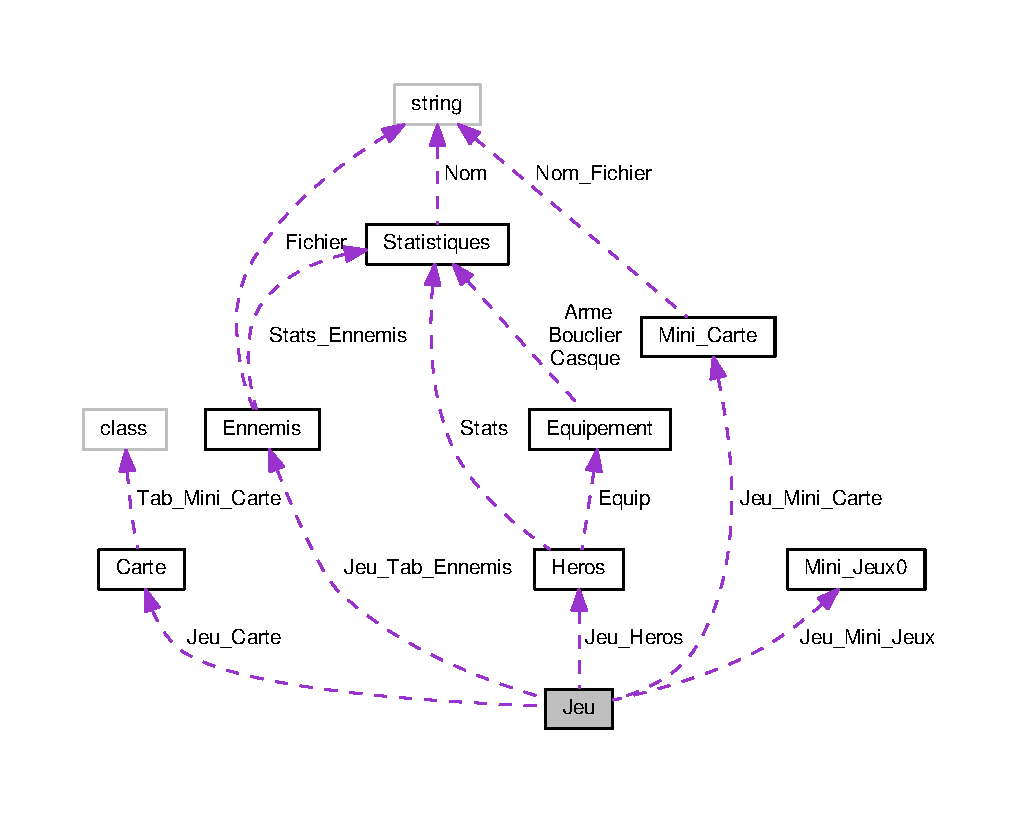
\includegraphics[width=350pt]{classJeu__coll__graph}
\end{center}
\end{figure}
\subsection*{Fonctions membres publiques}
\begin{DoxyCompactItemize}
\item 
\hypertarget{classJeu_a3c772a7fcdc7c9abe109ba41515e42c3}{\hyperlink{classCarte}{Carte} \& {\bfseries get\+\_\+\+Jeu\+\_\+\+Carte} ()}\label{classJeu_a3c772a7fcdc7c9abe109ba41515e42c3}

\item 
\hypertarget{classJeu_a944deec1fd22c99879921bee37d87eac}{\hyperlink{classMini__Carte}{Mini\+\_\+\+Carte} \& {\bfseries get\+\_\+\+Jeu\+\_\+\+Mini\+\_\+\+Carte} ()}\label{classJeu_a944deec1fd22c99879921bee37d87eac}

\item 
\hypertarget{classJeu_a98abd23fba88684cfb141c3159b14074}{\hyperlink{classHeros}{Heros} \& {\bfseries get\+\_\+\+Jeu\+\_\+\+Heros} ()}\label{classJeu_a98abd23fba88684cfb141c3159b14074}

\item 
\hypertarget{classJeu_a08e8f7ec1740bfdfd07e6ddc9c6985c9}{\hyperlink{classEnnemis}{Ennemis} \& {\bfseries get\+\_\+\+Jeu\+\_\+\+Tab\+\_\+\+Ennemis} (unsigned int i) const }\label{classJeu_a08e8f7ec1740bfdfd07e6ddc9c6985c9}

\item 
\hypertarget{classJeu_a600433d17f9474bfea664d43860a9853}{\hyperlink{classMini__Jeux0}{Mini\+\_\+\+Jeux0} {\bfseries get\+\_\+\+Jeu\+\_\+\+Mini\+\_\+\+Jeux} () const }\label{classJeu_a600433d17f9474bfea664d43860a9853}

\item 
\hypertarget{classJeu_a179a7776a4087957fe7e539522741a36}{const \hyperlink{classCarte}{Carte} \& {\bfseries get\+\_\+\+Const\+\_\+\+Jeu\+\_\+\+Carte} () const }\label{classJeu_a179a7776a4087957fe7e539522741a36}

\item 
\hypertarget{classJeu_ad7ff0fe6fa9af3c581305d6d07dba59b}{const \hyperlink{classMini__Carte}{Mini\+\_\+\+Carte} \& {\bfseries get\+\_\+\+Const\+\_\+\+Jeu\+\_\+\+Mini\+\_\+\+Carte} () const }\label{classJeu_ad7ff0fe6fa9af3c581305d6d07dba59b}

\item 
\hypertarget{classJeu_a91ec2b72f7046a1522fda3be53e8948c}{const \hyperlink{classHeros}{Heros} \& {\bfseries get\+\_\+\+Const\+\_\+\+Jeu\+\_\+\+Heros} () const }\label{classJeu_a91ec2b72f7046a1522fda3be53e8948c}

\item 
\hypertarget{classJeu_a1e420cba405c854a8392036bd75d751d}{const \hyperlink{classEnnemis}{Ennemis} \& {\bfseries get\+\_\+\+Const\+\_\+\+Jeu\+\_\+\+Tab\+\_\+\+Ennemis} () const }\label{classJeu_a1e420cba405c854a8392036bd75d751d}

\item 
\hypertarget{classJeu_adc630706f795ba4b9e3f34e6a022ec28}{const \hyperlink{classMini__Jeux0}{Mini\+\_\+\+Jeux0} {\bfseries get\+\_\+\+Const\+\_\+\+Jeu\+\_\+\+Mini\+\_\+\+Jeux} () const }\label{classJeu_adc630706f795ba4b9e3f34e6a022ec28}

\item 
\hypertarget{classJeu_ad83d41f74cedd43d21507698030a3cf4}{void {\bfseries Action\+\_\+\+Clavier} (const char touche, unsigned int \&position\+\_\+attaque\+\_\+magique\+\_\+x, unsigned int \&position\+\_\+attaque\+\_\+magique\+\_\+y, char \&orientation\+\_\+attaque\+\_\+magique)}\label{classJeu_ad83d41f74cedd43d21507698030a3cf4}

\item 
\hypertarget{classJeu_a55509208395374f443689dd04505b161}{void {\bfseries Action\+\_\+\+Automatique} (unsigned int \&vitesse\+\_\+attaque, unsigned int \&position\+\_\+attaque\+\_\+magique\+\_\+x, const unsigned int position\+\_\+attaque\+\_\+magique\+\_\+y, const char orientation\+\_\+attaque\+\_\+magique)}\label{classJeu_a55509208395374f443689dd04505b161}

\item 
\hypertarget{classJeu_ada702482e96105931c60b38ef7690755}{void \hyperlink{classJeu_ada702482e96105931c60b38ef7690755}{Modifie\+\_\+\+Stats\+\_\+heros} (unsigned int pourcentage)}\label{classJeu_ada702482e96105931c60b38ef7690755}

\begin{DoxyCompactList}\small\item\em Double les statistiques du héros après avoir gagné le mini jeu. \end{DoxyCompactList}\item 
\hypertarget{classJeu_ada6df09dbcf8f8d813606c16614e9f86}{void \hyperlink{classJeu_ada6df09dbcf8f8d813606c16614e9f86}{Mini\+\_\+\+Jeux\+\_\+\+Action\+\_\+\+Auto\+\_\+\+Avant\+\_\+\+Bouger} (unsigned int j, unsigned int a)}\label{classJeu_ada6df09dbcf8f8d813606c16614e9f86}

\begin{DoxyCompactList}\small\item\em Remplit la première ligne de blocs ou reste vide. \end{DoxyCompactList}\item 
\hypertarget{classJeu_a4813704613c198236c86c91c9ba9a859}{void \hyperlink{classJeu_a4813704613c198236c86c91c9ba9a859}{Mini\+\_\+\+Jeux\+\_\+\+Bouger} (char deplacement)}\label{classJeu_a4813704613c198236c86c91c9ba9a859}

\begin{DoxyCompactList}\small\item\em Permet au mini jeu de changer la position x,y du héros. \end{DoxyCompactList}\item 
\hypertarget{classJeu_aed47180f476f4d6d3271c184314eb79d}{bool \hyperlink{classJeu_aed47180f476f4d6d3271c184314eb79d}{Mini\+\_\+\+Jeux\+\_\+\+Action\+\_\+\+Auto\+\_\+\+Apres\+\_\+\+Bouger} (unsigned int k)}\label{classJeu_aed47180f476f4d6d3271c184314eb79d}

\begin{DoxyCompactList}\small\item\em Fait tomber les blocs d'une case et renvoie si le héros est écrasé ou non. \end{DoxyCompactList}\item 
\hypertarget{classJeu_aa0169feb94e7da99623bcf75d7eeef68}{void \hyperlink{classJeu_aa0169feb94e7da99623bcf75d7eeef68}{Mini\+\_\+\+Jeux\+\_\+\+Reinitialiser} ()}\label{classJeu_aa0169feb94e7da99623bcf75d7eeef68}

\begin{DoxyCompactList}\small\item\em Permet de remettre les données à leur état initial. \end{DoxyCompactList}\item 
\hypertarget{classJeu_a96aa5729378ab7b3a7974ef20da46043}{bool \hyperlink{classJeu_a96aa5729378ab7b3a7974ef20da46043}{Active\+\_\+\+Mini\+\_\+\+Jeux} ()}\label{classJeu_a96aa5729378ab7b3a7974ef20da46043}

\begin{DoxyCompactList}\small\item\em renvoie vraix si heros est dans zone remarquable ou pas \end{DoxyCompactList}\item 
\hypertarget{classJeu_a6a502f030e41b28604e5ffcd98e3ddd6}{void {\bfseries Au\+\_\+\+Bord} ()}\label{classJeu_a6a502f030e41b28604e5ffcd98e3ddd6}

\item 
\hypertarget{classJeu_a09ddc111dfdc9ec4531e32c0a63c0a05}{void {\bfseries set\+\_\+\+Jeu\+\_\+\+Mini\+\_\+\+Carte} (class \hyperlink{classMini__Carte}{Mini\+\_\+\+Carte} \&mini\+\_\+carte)}\label{classJeu_a09ddc111dfdc9ec4531e32c0a63c0a05}

\item 
\hypertarget{classJeu_a1fd894fb3e7ac370f8e3c0c3bc02fd49}{void \hyperlink{classJeu_a1fd894fb3e7ac370f8e3c0c3bc02fd49}{Lancement\+\_\+\+Jeu} ()}\label{classJeu_a1fd894fb3e7ac370f8e3c0c3bc02fd49}

\begin{DoxyCompactList}\small\item\em Définit comment le jeu est lancé \+: avec une sauvegarde ou en nouvelle partie P\+A\+S E\+N\+C\+O\+R\+E F\+A\+I\+T. \end{DoxyCompactList}\item 
\hypertarget{classJeu_ad2e3997a02c59546946aa45ddfc9fea2}{void \hyperlink{classJeu_ad2e3997a02c59546946aa45ddfc9fea2}{Debut\+\_\+\+Partie} ()}\label{classJeu_ad2e3997a02c59546946aa45ddfc9fea2}

\begin{DoxyCompactList}\small\item\em Amène le héros dans le hall et attend qu'il franchise la porte du donjon. \end{DoxyCompactList}\item 
\hypertarget{classJeu_afcb3c62eb261261aaacd2187cc83e120}{void \hyperlink{classJeu_afcb3c62eb261261aaacd2187cc83e120}{Labyrinthe} ()}\label{classJeu_afcb3c62eb261261aaacd2187cc83e120}

\begin{DoxyCompactList}\small\item\em Créer le labyrinthe. \end{DoxyCompactList}\item 
\hypertarget{classJeu_a26026d35f0a72ea75bb24ad687dfdeba}{void \hyperlink{classJeu_a26026d35f0a72ea75bb24ad687dfdeba}{Lance\+\_\+\+Mini\+\_\+\+Jeux} ()}\label{classJeu_a26026d35f0a72ea75bb24ad687dfdeba}

\begin{DoxyCompactList}\small\item\em Lance un mini-\/jeu. \end{DoxyCompactList}\item 
\hypertarget{classJeu_a6752dc9773b9bf400234de9cfe850cf9}{void {\bfseries Desaloc\+\_\+\+Jeu} ()}\label{classJeu_a6752dc9773b9bf400234de9cfe850cf9}

\item 
\hypertarget{classJeu_a9649f3bbfdfe0a505589eb322a9ed8a5}{void {\bfseries Desaloc\+\_\+\+Jeu\+\_\+\+Tab\+\_\+\+Ennemis} ()}\label{classJeu_a9649f3bbfdfe0a505589eb322a9ed8a5}

\item 
\hypertarget{classJeu_a6ae0cc96333dfbd7dd90c99829cdd45c}{void {\bfseries Recommence\+\_\+\+Jeu} ()}\label{classJeu_a6ae0cc96333dfbd7dd90c99829cdd45c}

\item 
\hypertarget{classJeu_a28c525fbd8621ae98a2ace2e81779365}{void {\bfseries Recupe\+\_\+\+Ennemis\+\_\+\+Mini\+\_\+\+Carte} ()}\label{classJeu_a28c525fbd8621ae98a2ace2e81779365}

\item 
\hypertarget{classJeu_ad6de5bb04656570f3a4168728566e15c}{int \hyperlink{classJeu_ad6de5bb04656570f3a4168728566e15c}{Recherche\+\_\+\+Ennemis} (unsigned int Position\+\_\+\+X, unsigned int Position\+\_\+\+Y)}\label{classJeu_ad6de5bb04656570f3a4168728566e15c}

\begin{DoxyCompactList}\small\item\em Fonction qui recherche itérativement l'ennemi qui possède ces coordonnées. \end{DoxyCompactList}\item 
\hypertarget{classJeu_a42deab2df34ecd40004f70aec777bf0b}{void \hyperlink{classJeu_a42deab2df34ecd40004f70aec777bf0b}{Supprime\+\_\+\+Ennemis} (unsigned int i)}\label{classJeu_a42deab2df34ecd40004f70aec777bf0b}

\begin{DoxyCompactList}\small\item\em Permet d'éliminer définitivement un ennemi(pas de réanimation lors du jeux sauf cas ou recommence jeu. \end{DoxyCompactList}\end{DoxyCompactItemize}
\subsection*{Attributs publics}
\begin{DoxyCompactItemize}
\item 
\hypertarget{classJeu_a542e022ef9c8f5de525d553ab5c2c4b5}{\hyperlink{classMini__Jeux0}{Mini\+\_\+\+Jeux0} {\bfseries Jeu\+\_\+\+Mini\+\_\+\+Jeux}}\label{classJeu_a542e022ef9c8f5de525d553ab5c2c4b5}

\end{DoxyCompactItemize}
\subsection*{Attributs privés}
\begin{DoxyCompactItemize}
\item 
\hypertarget{classJeu_a653e9003649e8e52a97b7bb0687dbb45}{\hyperlink{classCarte}{Carte} {\bfseries Jeu\+\_\+\+Carte}}\label{classJeu_a653e9003649e8e52a97b7bb0687dbb45}

\item 
\hypertarget{classJeu_af74402ca4ee6eeadd483a1576db1662a}{\hyperlink{classHeros}{Heros} {\bfseries Jeu\+\_\+\+Heros}}\label{classJeu_af74402ca4ee6eeadd483a1576db1662a}

\item 
\hypertarget{classJeu_a42766cc97bc1fbc987f36c3eb7d6664c}{\hyperlink{classEnnemis}{Ennemis} $\ast$ {\bfseries Jeu\+\_\+\+Tab\+\_\+\+Ennemis}}\label{classJeu_a42766cc97bc1fbc987f36c3eb7d6664c}

\item 
\hypertarget{classJeu_a9ca8a3168105db0f97b725a9c0e59067}{\hyperlink{classMini__Carte}{Mini\+\_\+\+Carte} {\bfseries Jeu\+\_\+\+Mini\+\_\+\+Carte}}\label{classJeu_a9ca8a3168105db0f97b725a9c0e59067}

\end{DoxyCompactItemize}


La documentation de cette classe a été générée à partir des fichiers suivants \+:\begin{DoxyCompactItemize}
\item 
src/include/Jeu.\+h\item 
src/cpp/Jeu.\+cpp\end{DoxyCompactItemize}

\hypertarget{classMini__Carte}{\section{Référence de la classe Mini\+\_\+\+Carte}
\label{classMini__Carte}\index{Mini\+\_\+\+Carte@{Mini\+\_\+\+Carte}}
}


Graphe de collaboration de Mini\+\_\+\+Carte\+:\nopagebreak
\begin{figure}[H]
\begin{center}
\leavevmode
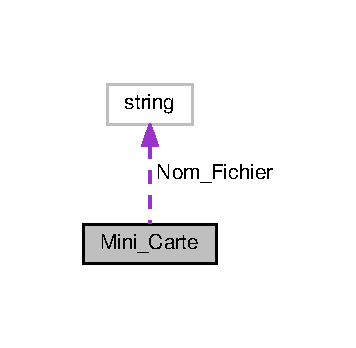
\includegraphics[width=171pt]{classMini__Carte__coll__graph}
\end{center}
\end{figure}
\subsection*{Fonctions membres publiques}
\begin{DoxyCompactItemize}
\item 
\hypertarget{classMini__Carte_aaf8ff27aeacc064c4d5d624316f6ff1f}{\hyperlink{classMini__Carte_aaf8ff27aeacc064c4d5d624316f6ff1f}{Mini\+\_\+\+Carte} ()}\label{classMini__Carte_aaf8ff27aeacc064c4d5d624316f6ff1f}

\begin{DoxyCompactList}\small\item\em Constructeur par défaut. \end{DoxyCompactList}\item 
\hypertarget{classMini__Carte_a8b4f208bc954b0e5591a429e3fab4ff6}{\hyperlink{classMini__Carte_a8b4f208bc954b0e5591a429e3fab4ff6}{Mini\+\_\+\+Carte} (string Nom\+\_\+\+Fich)}\label{classMini__Carte_a8b4f208bc954b0e5591a429e3fab4ff6}

\begin{DoxyCompactList}\small\item\em Constructeur d'une carte par rapport à un fichier. \end{DoxyCompactList}\item 
\hypertarget{classMini__Carte_a0a1df1661df087726886947c67cdc102}{\hyperlink{classMini__Carte_a0a1df1661df087726886947c67cdc102}{$\sim$\+Mini\+\_\+\+Carte} ()}\label{classMini__Carte_a0a1df1661df087726886947c67cdc102}

\begin{DoxyCompactList}\small\item\em Destructeur par défaut. \end{DoxyCompactList}\item 
\hypertarget{classMini__Carte_a30139202067e4c75e278598925654613}{void \hyperlink{classMini__Carte_a30139202067e4c75e278598925654613}{Desaloc\+\_\+\+Tab} ()}\label{classMini__Carte_a30139202067e4c75e278598925654613}

\begin{DoxyCompactList}\small\item\em Désalloue les deux tableaux. \end{DoxyCompactList}\item 
\hypertarget{classMini__Carte_a71a52a8ec4d894d394e79e8e24543822}{void \hyperlink{classMini__Carte_a71a52a8ec4d894d394e79e8e24543822}{Alloc\+\_\+\+Tab} (unsigned int x, unsigned int y)}\label{classMini__Carte_a71a52a8ec4d894d394e79e8e24543822}

\begin{DoxyCompactList}\small\item\em Alloue le tableau (x et y dim de mini carte) \end{DoxyCompactList}\item 
\hypertarget{classMini__Carte_a8a9e758328f7c0f66e22db4cbb2bcf6b}{void {\bfseries Ouvrir\+\_\+\+Mini\+\_\+\+Carte} (string nom\+\_\+fichier)}\label{classMini__Carte_a8a9e758328f7c0f66e22db4cbb2bcf6b}

\item 
\hypertarget{classMini__Carte_ad1e6f929c742503fc7b5d00872dff6dd}{unsigned int \hyperlink{classMini__Carte_ad1e6f929c742503fc7b5d00872dff6dd}{get\+\_\+\+Tab\+\_\+\+Mini\+\_\+\+Carte} (unsigned int x, unsigned int y) const }\label{classMini__Carte_ad1e6f929c742503fc7b5d00872dff6dd}

\begin{DoxyCompactList}\small\item\em Retourne l'entier du tableau de jeu de la xème ligne et yème colonne. \end{DoxyCompactList}\item 
\hypertarget{classMini__Carte_ada7f3e49014f9a84e1d83918f6270753}{unsigned int \hyperlink{classMini__Carte_ada7f3e49014f9a84e1d83918f6270753}{get\+\_\+\+Taille\+\_\+\+Mini\+\_\+\+Carte\+\_\+\+X} () const }\label{classMini__Carte_ada7f3e49014f9a84e1d83918f6270753}

\begin{DoxyCompactList}\small\item\em Retourne la longueur (taille horizontale) de la mini-\/carte. \end{DoxyCompactList}\item 
\hypertarget{classMini__Carte_aa2613563aa665346d17ad8299d6b35ac}{unsigned int \hyperlink{classMini__Carte_aa2613563aa665346d17ad8299d6b35ac}{get\+\_\+\+Taille\+\_\+\+Mini\+\_\+\+Carte\+\_\+\+Y} () const }\label{classMini__Carte_aa2613563aa665346d17ad8299d6b35ac}

\begin{DoxyCompactList}\small\item\em Retourne la largeur (taille verticale) de la mini-\/carte. \end{DoxyCompactList}\item 
\hypertarget{classMini__Carte_aa41531fea4c1d153a12252cc5338d140}{unsigned int \hyperlink{classMini__Carte_aa41531fea4c1d153a12252cc5338d140}{get\+\_\+\+Nombre\+\_\+\+Ennemis} () const }\label{classMini__Carte_aa41531fea4c1d153a12252cc5338d140}

\begin{DoxyCompactList}\small\item\em Retourne le nombre d'ennemis présents sur la mini-\/carte. \end{DoxyCompactList}\item 
\hypertarget{classMini__Carte_a4186d56afe409cb52e021a8ad6a6ca37}{void \hyperlink{classMini__Carte_a4186d56afe409cb52e021a8ad6a6ca37}{get\+\_\+\+Nom\+\_\+\+Fichier} (string \hyperlink{classMini__Carte_ad428c788dfb171b10f7a7f8153498475}{Nom\+\_\+\+Fichier}) const }\label{classMini__Carte_a4186d56afe409cb52e021a8ad6a6ca37}

\begin{DoxyCompactList}\small\item\em Retouren le nom du fichier. \end{DoxyCompactList}\item 
\hypertarget{classMini__Carte_a45e670383712f3a72ee735cd9e834a73}{void \hyperlink{classMini__Carte_a45e670383712f3a72ee735cd9e834a73}{get\+\_\+\+Mini\+\_\+\+Carte} (\hyperlink{classMini__Carte}{Mini\+\_\+\+Carte} \&mini\+\_\+carte) const }\label{classMini__Carte_a45e670383712f3a72ee735cd9e834a73}

\begin{DoxyCompactList}\small\item\em Retourne dans mini\+\_\+carte la mini carte actuelle. \end{DoxyCompactList}\item 
\hypertarget{classMini__Carte_adec3615384b8128e9281319b460ad7a2}{void \hyperlink{classMini__Carte_adec3615384b8128e9281319b460ad7a2}{set\+\_\+\+Tab\+\_\+\+Mini\+\_\+\+Carte} (unsigned int x, unsigned int y, unsigned int entier\+\_\+a\+\_\+mettre)}\label{classMini__Carte_adec3615384b8128e9281319b460ad7a2}

\begin{DoxyCompactList}\small\item\em Transforme l'entier de la xème ligne et yème colonne en entier\+\_\+a\+\_\+mettre. \end{DoxyCompactList}\item 
\hypertarget{classMini__Carte_a9d138ed93e2df25c4b7ef88d099c2665}{void \hyperlink{classMini__Carte_a9d138ed93e2df25c4b7ef88d099c2665}{set\+\_\+\+Nom\+\_\+\+Fichier} (string nom\+\_\+fichier)}\label{classMini__Carte_a9d138ed93e2df25c4b7ef88d099c2665}

\begin{DoxyCompactList}\small\item\em Modifie le nom du fichier. \end{DoxyCompactList}\item 
\hypertarget{classMini__Carte_a6341b67077c2ba0052d18da053cacca2}{void \hyperlink{classMini__Carte_a6341b67077c2ba0052d18da053cacca2}{set\+\_\+\+Taille\+\_\+\+Mini\+\_\+\+Carte\+\_\+\+X} (unsigned int x)}\label{classMini__Carte_a6341b67077c2ba0052d18da053cacca2}

\begin{DoxyCompactList}\small\item\em Edite la taille horizontale de la mini-\/carte. \end{DoxyCompactList}\item 
\hypertarget{classMini__Carte_ae7b923e190866aa72bbc9e519b97113f}{void \hyperlink{classMini__Carte_ae7b923e190866aa72bbc9e519b97113f}{set\+\_\+\+Taille\+\_\+\+Mini\+\_\+\+Carte\+\_\+\+Y} (unsigned int y)}\label{classMini__Carte_ae7b923e190866aa72bbc9e519b97113f}

\begin{DoxyCompactList}\small\item\em Edite la taille verticale de la mini-\/carte. \end{DoxyCompactList}\item 
\hypertarget{classMini__Carte_aca5011429573ab481e1da9e71f66da5c}{void \hyperlink{classMini__Carte_aca5011429573ab481e1da9e71f66da5c}{set\+\_\+\+Nombre\+\_\+\+Ennemis} (unsigned int nb\+\_\+ennemis)}\label{classMini__Carte_aca5011429573ab481e1da9e71f66da5c}

\begin{DoxyCompactList}\small\item\em Edite le nombre d'ennemis présents sur la mini-\/carte. \end{DoxyCompactList}\item 
\hypertarget{classMini__Carte_a44f5923497dd845749a99e635acc5862}{void \hyperlink{classMini__Carte_a44f5923497dd845749a99e635acc5862}{set\+\_\+\+Mini\+\_\+\+Carte} (const \hyperlink{classMini__Carte}{Mini\+\_\+\+Carte} \&mini\+\_\+carte)}\label{classMini__Carte_a44f5923497dd845749a99e635acc5862}

\begin{DoxyCompactList}\small\item\em Modification de la mini carte en mini\+\_\+carte. \end{DoxyCompactList}\item 
\hypertarget{classMini__Carte_a33143aaed2795104e7f73ae9f3a9186c}{void \hyperlink{classMini__Carte_a33143aaed2795104e7f73ae9f3a9186c}{Affiche\+\_\+\+Mini\+\_\+\+Carte} () const }\label{classMini__Carte_a33143aaed2795104e7f73ae9f3a9186c}

\begin{DoxyCompactList}\small\item\em Affiche la mini carte de jeu en entier. \end{DoxyCompactList}\item 
\hypertarget{classMini__Carte_aef613418e12a631e3512f3d031d9a724}{void \hyperlink{classMini__Carte_aef613418e12a631e3512f3d031d9a724}{Affiche\+\_\+\+Non\+\_\+\+Vide} () const }\label{classMini__Carte_aef613418e12a631e3512f3d031d9a724}

\begin{DoxyCompactList}\small\item\em Affiche les murs de la mini carte et met des espaces sur le(s) zones vides. \end{DoxyCompactList}\item 
\hypertarget{classMini__Carte_a646384624b968c675b5f8be52ceb73ad}{bool \hyperlink{classMini__Carte_a646384624b968c675b5f8be52ceb73ad}{Est\+\_\+\+Ce\+\_\+\+Que\+\_\+\+Mur} (unsigned int x, unsigned int y) const }\label{classMini__Carte_a646384624b968c675b5f8be52ceb73ad}

\begin{DoxyCompactList}\small\item\em Vérifie s'il y a un mur en face du personnage (héros ou ennemi) \end{DoxyCompactList}\item 
\hypertarget{classMini__Carte_a9da689c43f60b07dd3b113de2b6ca312}{bool \hyperlink{classMini__Carte_a9da689c43f60b07dd3b113de2b6ca312}{Est\+\_\+\+Ce\+\_\+\+Que\+\_\+\+Plateforme} (unsigned int x, unsigned int y) const }\label{classMini__Carte_a9da689c43f60b07dd3b113de2b6ca312}

\begin{DoxyCompactList}\small\item\em Vérifie s'il y a une plateforme accessible pour le personnage (héros ou ennemi) \end{DoxyCompactList}\item 
\hypertarget{classMini__Carte_a3a045e6289f6a58665fef737d0cb9ca7}{bool \hyperlink{classMini__Carte_a3a045e6289f6a58665fef737d0cb9ca7}{Est\+\_\+\+Ce\+\_\+\+Que\+\_\+\+Vide} (unsigned int x, unsigned int y) const }\label{classMini__Carte_a3a045e6289f6a58665fef737d0cb9ca7}

\begin{DoxyCompactList}\small\item\em Vérifie si l'emplacement est vide pour pouvoir y accéder. \end{DoxyCompactList}\end{DoxyCompactItemize}
\subsection*{Attributs privés}
\begin{DoxyCompactItemize}
\item 
\hypertarget{classMini__Carte_ad428c788dfb171b10f7a7f8153498475}{string \hyperlink{classMini__Carte_ad428c788dfb171b10f7a7f8153498475}{Nom\+\_\+\+Fichier}}\label{classMini__Carte_ad428c788dfb171b10f7a7f8153498475}

\begin{DoxyCompactList}\small\item\em Nom (avec extension) du fichier qui permet d'ouvrir/sauvegarder une mini carte. \end{DoxyCompactList}\item 
\hypertarget{classMini__Carte_a59fed7ef487bae072e47c6898ee1f807}{unsigned int $\ast$ \hyperlink{classMini__Carte_a59fed7ef487bae072e47c6898ee1f807}{Tab\+\_\+\+Mini\+\_\+\+Carte}}\label{classMini__Carte_a59fed7ef487bae072e47c6898ee1f807}

\begin{DoxyCompactList}\small\item\em Tableau représentant une zone jouable du jeu. \end{DoxyCompactList}\item 
\hypertarget{classMini__Carte_a42d3fb10ef213e81417be02af11db56b}{unsigned int \hyperlink{classMini__Carte_a42d3fb10ef213e81417be02af11db56b}{Taille\+\_\+\+Mini\+\_\+\+Carte\+\_\+\+X}}\label{classMini__Carte_a42d3fb10ef213e81417be02af11db56b}

\begin{DoxyCompactList}\small\item\em Valeur représentant la taille horizontale de la mini-\/carte. \end{DoxyCompactList}\item 
\hypertarget{classMini__Carte_a4c62f6e1912da87652645dd70d0fde8f}{unsigned int \hyperlink{classMini__Carte_a4c62f6e1912da87652645dd70d0fde8f}{Taille\+\_\+\+Mini\+\_\+\+Carte\+\_\+\+Y}}\label{classMini__Carte_a4c62f6e1912da87652645dd70d0fde8f}

\begin{DoxyCompactList}\small\item\em Valeur représentant la taille horizontale de la mini-\/carte. \end{DoxyCompactList}\item 
\hypertarget{classMini__Carte_a348d0f6a599e8dc5bacda2150b8dd5d0}{unsigned int \hyperlink{classMini__Carte_a348d0f6a599e8dc5bacda2150b8dd5d0}{Nombre\+\_\+\+Ennemis}}\label{classMini__Carte_a348d0f6a599e8dc5bacda2150b8dd5d0}

\begin{DoxyCompactList}\small\item\em Nombre d'ennemis sur la mini carte. \end{DoxyCompactList}\end{DoxyCompactItemize}


La documentation de cette classe a été générée à partir des fichiers suivants \+:\begin{DoxyCompactItemize}
\item 
src/include/Mini\+\_\+\+Carte.\+h\item 
src/cpp/Mini\+\_\+\+Carte.\+cpp\end{DoxyCompactItemize}

\hypertarget{classMini__Jeux0}{\section{Référence de la classe Mini\+\_\+\+Jeux0}
\label{classMini__Jeux0}\index{Mini\+\_\+\+Jeux0@{Mini\+\_\+\+Jeux0}}
}
\subsection*{Fonctions membres publiques}
\begin{DoxyCompactItemize}
\item 
\hypertarget{classMini__Jeux0_ae78bb59539618b9e8fbf56e9c24351b9}{const unsigned int \hyperlink{classMini__Jeux0_ae78bb59539618b9e8fbf56e9c24351b9}{get\+\_\+\+Position\+\_\+\+X} () const }\label{classMini__Jeux0_ae78bb59539618b9e8fbf56e9c24351b9}

\begin{DoxyCompactList}\small\item\em renvoie la position x du heros du minijeux \end{DoxyCompactList}\item 
\hypertarget{classMini__Jeux0_a96ce7038496cc16b6a3d887c629d2d52}{const unsigned int \hyperlink{classMini__Jeux0_a96ce7038496cc16b6a3d887c629d2d52}{get\+\_\+\+Position\+\_\+\+Y} () const }\label{classMini__Jeux0_a96ce7038496cc16b6a3d887c629d2d52}

\begin{DoxyCompactList}\small\item\em renvoie la position y du heros du minijeux \end{DoxyCompactList}\item 
\hypertarget{classMini__Jeux0_a6fa903b50720fddd886c8e09668ba47d}{const unsigned int \hyperlink{classMini__Jeux0_a6fa903b50720fddd886c8e09668ba47d}{get\+\_\+\+Tab} (unsigned int x, unsigned int y) const }\label{classMini__Jeux0_a6fa903b50720fddd886c8e09668ba47d}

\begin{DoxyCompactList}\small\item\em Retourne l'entier du tableau de jeu de la x�me ligne et y�me colonne. \end{DoxyCompactList}\item 
\hypertarget{classMini__Jeux0_a3f1db24c33cde12323c87ba1fd553aad}{void \hyperlink{classMini__Jeux0_a3f1db24c33cde12323c87ba1fd553aad}{set\+\_\+\+Position\+\_\+\+X} (unsigned int Position\+\_\+\+X)}\label{classMini__Jeux0_a3f1db24c33cde12323c87ba1fd553aad}

\begin{DoxyCompactList}\small\item\em accede � la position x du heros du minijeux \end{DoxyCompactList}\item 
\hypertarget{classMini__Jeux0_a7d93665cb137680907a23dfa8b4dc334}{void \hyperlink{classMini__Jeux0_a7d93665cb137680907a23dfa8b4dc334}{set\+\_\+\+Position\+\_\+\+Y} (unsigned int Position\+\_\+\+Y)}\label{classMini__Jeux0_a7d93665cb137680907a23dfa8b4dc334}

\begin{DoxyCompactList}\small\item\em accede � la position y du heros du minijeux \end{DoxyCompactList}\item 
\hypertarget{classMini__Jeux0_aa3a26649ffb079f98cf2252f654cf73f}{void \hyperlink{classMini__Jeux0_aa3a26649ffb079f98cf2252f654cf73f}{set\+\_\+\+Tab} (unsigned int x, unsigned int y, unsigned int entier)}\label{classMini__Jeux0_aa3a26649ffb079f98cf2252f654cf73f}

\begin{DoxyCompactList}\small\item\em modifie l'entier de la x�me ligne et y�me colonne en entier\+\_\+a\+\_\+mettre \end{DoxyCompactList}\item 
\hypertarget{classMini__Jeux0_ae27cd352ee1644e8649013fd609e9020}{bool \hyperlink{classMini__Jeux0_ae27cd352ee1644e8649013fd609e9020}{Tombe} (unsigned int k)}\label{classMini__Jeux0_ae27cd352ee1644e8649013fd609e9020}

\begin{DoxyCompactList}\small\item\em fais tomber les meteorite d'une ligne \end{DoxyCompactList}\item 
\hypertarget{classMini__Jeux0_ae7c51f1c431841bcf8b58e5eff9f445d}{void \hyperlink{classMini__Jeux0_ae7c51f1c431841bcf8b58e5eff9f445d}{Bouger} (char deplacement)}\label{classMini__Jeux0_ae7c51f1c431841bcf8b58e5eff9f445d}

\begin{DoxyCompactList}\small\item\em fais bouger le perso sur les comande g gauche et d droite et rien le perso ne bouge pas (changer par le sdl qui l'apel) \end{DoxyCompactList}\item 
\hypertarget{classMini__Jeux0_ad2969d288ffe43404350d298fc8029d9}{bool \hyperlink{classMini__Jeux0_ad2969d288ffe43404350d298fc8029d9}{Jeu} (string filename)}\label{classMini__Jeux0_ad2969d288ffe43404350d298fc8029d9}

\begin{DoxyCompactList}\small\item\em ancien fonctionnement du jeu quelque modifications du mini\+\_\+jeux pour s'implementer dans un autre jeu il suis l'implementation du jeu \end{DoxyCompactList}\item 
\hypertarget{classMini__Jeux0_a024bc7862a9ca9aee48750c929edc012}{void \hyperlink{classMini__Jeux0_a024bc7862a9ca9aee48750c929edc012}{Tour} (unsigned int tab\mbox{[}Taille\mbox{]}\mbox{[}Taille\mbox{]}, string \&filename)}\label{classMini__Jeux0_a024bc7862a9ca9aee48750c929edc012}

\begin{DoxyCompactList}\small\item\em remplie la premier ligne d'un tableau a partir d'un fichier P\+A\+S U\+T\+I\+L\+I\+S\+E\+R \end{DoxyCompactList}\item 
\hypertarget{classMini__Jeux0_aacacc639047611a7f8ea2eb2488fb5b1}{void \hyperlink{classMini__Jeux0_aacacc639047611a7f8ea2eb2488fb5b1}{Afficher} (unsigned int tab\mbox{[}Taille\mbox{]}\mbox{[}Taille\mbox{]})}\label{classMini__Jeux0_aacacc639047611a7f8ea2eb2488fb5b1}

\begin{DoxyCompactList}\small\item\em sert a afficher le jeu \end{DoxyCompactList}\item 
\hypertarget{classMini__Jeux0_a0f23d8a9c13f7f9454da73e59a164a14}{void {\bfseries Test\+\_\+\+Regression} ()}\label{classMini__Jeux0_a0f23d8a9c13f7f9454da73e59a164a14}

\item 
\hyperlink{classMini__Jeux0_a35b3a9818d33633c46c7deb22509112c}{Mini\+\_\+\+Jeux0} ()
\item 
virtual \hyperlink{classMini__Jeux0_a390c8c673e8295bf0ecaa094e25a0080}{$\sim$\+Mini\+\_\+\+Jeux0} ()
\end{DoxyCompactItemize}
\subsection*{Attributs privés}
\begin{DoxyCompactItemize}
\item 
\hypertarget{classMini__Jeux0_ac15cbe9345fb410567fab8d77e327825}{unsigned int {\bfseries tab} \mbox{[}Taille\mbox{]}\mbox{[}Taille\mbox{]}}\label{classMini__Jeux0_ac15cbe9345fb410567fab8d77e327825}

\item 
\hypertarget{classMini__Jeux0_a10407c036869081505d063369f540005}{unsigned int {\bfseries Position\+\_\+\+X}}\label{classMini__Jeux0_a10407c036869081505d063369f540005}

\item 
\hypertarget{classMini__Jeux0_a57076f898b39d426a53c286474fb4779}{unsigned int {\bfseries Position\+\_\+\+Y}}\label{classMini__Jeux0_a57076f898b39d426a53c286474fb4779}

\end{DoxyCompactItemize}


\subsection{Documentation des constructeurs et destructeur}
\hypertarget{classMini__Jeux0_a35b3a9818d33633c46c7deb22509112c}{\index{Mini\+\_\+\+Jeux0@{Mini\+\_\+\+Jeux0}!Mini\+\_\+\+Jeux0@{Mini\+\_\+\+Jeux0}}
\index{Mini\+\_\+\+Jeux0@{Mini\+\_\+\+Jeux0}!Mini\+\_\+\+Jeux0@{Mini\+\_\+\+Jeux0}}
\subsubsection[{Mini\+\_\+\+Jeux0}]{\setlength{\rightskip}{0pt plus 5cm}Mini\+\_\+\+Jeux0\+::\+Mini\+\_\+\+Jeux0 (
\begin{DoxyParamCaption}
{}
\end{DoxyParamCaption}
)}}\label{classMini__Jeux0_a35b3a9818d33633c46c7deb22509112c}
Default constructor \hypertarget{classMini__Jeux0_a390c8c673e8295bf0ecaa094e25a0080}{\index{Mini\+\_\+\+Jeux0@{Mini\+\_\+\+Jeux0}!````~Mini\+\_\+\+Jeux0@{$\sim$\+Mini\+\_\+\+Jeux0}}
\index{````~Mini\+\_\+\+Jeux0@{$\sim$\+Mini\+\_\+\+Jeux0}!Mini\+\_\+\+Jeux0@{Mini\+\_\+\+Jeux0}}
\subsubsection[{$\sim$\+Mini\+\_\+\+Jeux0}]{\setlength{\rightskip}{0pt plus 5cm}Mini\+\_\+\+Jeux0\+::$\sim$\+Mini\+\_\+\+Jeux0 (
\begin{DoxyParamCaption}
{}
\end{DoxyParamCaption}
)\hspace{0.3cm}{\ttfamily [virtual]}}}\label{classMini__Jeux0_a390c8c673e8295bf0ecaa094e25a0080}
Default destructor 

La documentation de cette classe a été générée à partir des fichiers suivants \+:\begin{DoxyCompactItemize}
\item 
src/include/Mini\+\_\+\+Jeux0.\+h\item 
src/cpp/Mini\+\_\+\+Jeux0.\+cpp\end{DoxyCompactItemize}

\hypertarget{classObjet}{\section{Référence de la classe Objet}
\label{classObjet}\index{Objet@{Objet}}
}


Graphe de collaboration de Objet\+:\nopagebreak
\begin{figure}[H]
\begin{center}
\leavevmode
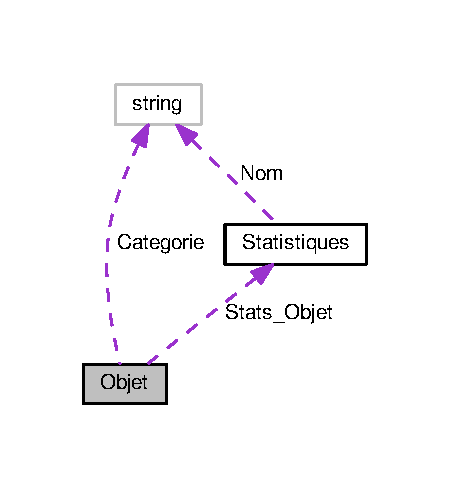
\includegraphics[width=216pt]{classObjet__coll__graph}
\end{center}
\end{figure}
\subsection*{Fonctions membres publiques}
\begin{DoxyCompactItemize}
\item 
\hyperlink{classObjet_aefdd826d50085897e4894ffef4597d04}{Objet} ()
\item 
\hypertarget{classObjet_a6c77475820cefde8ce21f50913980611}{\hyperlink{classObjet_a6c77475820cefde8ce21f50913980611}{Objet} (string categorie, \hyperlink{classStatistiques}{Statistiques} stats\+\_\+objet)}\label{classObjet_a6c77475820cefde8ce21f50913980611}

\begin{DoxyCompactList}\small\item\em Constructeur par param�tre. \end{DoxyCompactList}\item 
virtual \hyperlink{classObjet_a8d9fa6fa05b9f5a99ab60d08f6b558ee}{$\sim$\+Objet} ()
\item 
\hypertarget{classObjet_a9fffc01eb7857beb33e44c3dbc71ae5d}{string \hyperlink{classObjet_a9fffc01eb7857beb33e44c3dbc71ae5d}{get\+\_\+\+Categorie} () const }\label{classObjet_a9fffc01eb7857beb33e44c3dbc71ae5d}

\begin{DoxyCompactList}\small\item\em Retourne la cat�gorie. \end{DoxyCompactList}\item 
\hypertarget{classObjet_ac03dffee3b2b3e951c333fa9cd93900e}{\hyperlink{classStatistiques}{Statistiques} \hyperlink{classObjet_ac03dffee3b2b3e951c333fa9cd93900e}{get\+\_\+\+Stats\+\_\+\+Objet} () const }\label{classObjet_ac03dffee3b2b3e951c333fa9cd93900e}

\begin{DoxyCompactList}\small\item\em Retourne la cat�gorie. \end{DoxyCompactList}\item 
\hypertarget{classObjet_a6be177ae5ff07fec50fa26fc79693480}{string \hyperlink{classObjet_a6be177ae5ff07fec50fa26fc79693480}{get\+\_\+\+Stats\+\_\+\+Objet\+\_\+\+Nom} () const }\label{classObjet_a6be177ae5ff07fec50fa26fc79693480}

\begin{DoxyCompactList}\small\item\em Modifie la donn�e membre Stats\+\_\+\+Objet.\+Nom. \end{DoxyCompactList}\item 
\hypertarget{classObjet_a34a298c74077fe044ecfff40855f6e5f}{unsigned int \hyperlink{classObjet_a34a298c74077fe044ecfff40855f6e5f}{get\+\_\+\+Stats\+\_\+\+Objet\+\_\+\+Point\+\_\+\+De\+\_\+\+Vie} () const }\label{classObjet_a34a298c74077fe044ecfff40855f6e5f}

\begin{DoxyCompactList}\small\item\em Modifie la donn�e membre Stats\+\_\+\+Objet.\+Point\+\_\+\+De\+\_\+\+Vie. \end{DoxyCompactList}\item 
\hypertarget{classObjet_a230f04bb73a299548f05980ea5a1e6b2}{unsigned int \hyperlink{classObjet_a230f04bb73a299548f05980ea5a1e6b2}{get\+\_\+\+Stats\+\_\+\+Objet\+\_\+\+Point\+\_\+\+De\+\_\+\+Vie\+\_\+\+Max} () const }\label{classObjet_a230f04bb73a299548f05980ea5a1e6b2}

\begin{DoxyCompactList}\small\item\em Modifie la donn�e membre Stats\+\_\+\+Objet.\+Point\+\_\+\+De\+\_\+\+Vie\+\_\+\+Max. \end{DoxyCompactList}\item 
\hypertarget{classObjet_a8c47bc9047dea7758a39c47de801058d}{unsigned int \hyperlink{classObjet_a8c47bc9047dea7758a39c47de801058d}{get\+\_\+\+Stats\+\_\+\+Objet\+\_\+\+Mana} () const }\label{classObjet_a8c47bc9047dea7758a39c47de801058d}

\begin{DoxyCompactList}\small\item\em Modifie la donn�e membre Stats\+\_\+\+Objet.\+Mana. \end{DoxyCompactList}\item 
\hypertarget{classObjet_aeaf0f0061830388980e4a1ddec26e9f8}{unsigned int \hyperlink{classObjet_aeaf0f0061830388980e4a1ddec26e9f8}{get\+\_\+\+Stats\+\_\+\+Objet\+\_\+\+Mana\+\_\+\+Max} () const }\label{classObjet_aeaf0f0061830388980e4a1ddec26e9f8}

\begin{DoxyCompactList}\small\item\em Modifie la donn�e membre Stats\+\_\+\+Objet.\+Mana\+\_\+\+Max. \end{DoxyCompactList}\item 
\hypertarget{classObjet_a3f719e06a9c20fe56dbb6def9da0c175}{unsigned int \hyperlink{classObjet_a3f719e06a9c20fe56dbb6def9da0c175}{get\+\_\+\+Stats\+\_\+\+Objet\+\_\+\+Experience\+\_\+\+Restant} () const }\label{classObjet_a3f719e06a9c20fe56dbb6def9da0c175}

\begin{DoxyCompactList}\small\item\em Modifie la donn�e membre Stats\+\_\+\+Objet.\+Experience\+\_\+\+Restant. \end{DoxyCompactList}\item 
\hypertarget{classObjet_a872678f7cb4f103c7bc4de4efbf14b66}{unsigned int \hyperlink{classObjet_a872678f7cb4f103c7bc4de4efbf14b66}{get\+\_\+\+Stats\+\_\+\+Objet\+\_\+\+Experience\+\_\+\+Donne} () const }\label{classObjet_a872678f7cb4f103c7bc4de4efbf14b66}

\begin{DoxyCompactList}\small\item\em Retourne la donn�e membre Stats\+\_\+\+Objet.\+Experience\+\_\+\+Restant. \end{DoxyCompactList}\item 
\hypertarget{classObjet_af6912f94de376852cba77213be31bfe1}{unsigned int \hyperlink{classObjet_af6912f94de376852cba77213be31bfe1}{get\+\_\+\+Stats\+\_\+\+Objet\+\_\+\+Niveau} () const }\label{classObjet_af6912f94de376852cba77213be31bfe1}

\begin{DoxyCompactList}\small\item\em Retourne la donn�e membre Stats\+\_\+\+Objet.\+Niveaux. \end{DoxyCompactList}\item 
\hypertarget{classObjet_ad39dacfd50a5ada4af55700f59b5e175}{unsigned int \hyperlink{classObjet_ad39dacfd50a5ada4af55700f59b5e175}{get\+\_\+\+Stats\+\_\+\+Objet\+\_\+\+Force} () const }\label{classObjet_ad39dacfd50a5ada4af55700f59b5e175}

\begin{DoxyCompactList}\small\item\em Retourne la donn�e membre Stats\+\_\+\+Objet.\+Force. \end{DoxyCompactList}\item 
\hypertarget{classObjet_a33f8a589e75a1368f15b256a141f941f}{unsigned int \hyperlink{classObjet_a33f8a589e75a1368f15b256a141f941f}{get\+\_\+\+Stats\+\_\+\+Objet\+\_\+\+Intelligence} () const }\label{classObjet_a33f8a589e75a1368f15b256a141f941f}

\begin{DoxyCompactList}\small\item\em Retourne la donn�e membre Stats\+\_\+\+Objet.\+Intelligence. \end{DoxyCompactList}\item 
\hypertarget{classObjet_a6f12fadbfb6fcd694fe532608c4fcd00}{unsigned int \hyperlink{classObjet_a6f12fadbfb6fcd694fe532608c4fcd00}{get\+\_\+\+Stats\+\_\+\+Objet\+\_\+\+Agilite} () const }\label{classObjet_a6f12fadbfb6fcd694fe532608c4fcd00}

\begin{DoxyCompactList}\small\item\em Retourne la donn�e membre Stats\+\_\+\+Objet.\+agilite. \end{DoxyCompactList}\item 
\hypertarget{classObjet_a13251bc8211aa2a62e288311451ba7e5}{void \hyperlink{classObjet_a13251bc8211aa2a62e288311451ba7e5}{set\+\_\+\+Categorie} (string categorie)}\label{classObjet_a13251bc8211aa2a62e288311451ba7e5}

\begin{DoxyCompactList}\small\item\em Modifie a la donn� membre Categorie. \end{DoxyCompactList}\item 
\hypertarget{classObjet_aa977cb20177c63d3136c84bd8d1bd865}{void \hyperlink{classObjet_aa977cb20177c63d3136c84bd8d1bd865}{set\+\_\+\+Stats\+\_\+\+Objet} (\hyperlink{classStatistiques}{Statistiques} stats\+\_\+objet)}\label{classObjet_aa977cb20177c63d3136c84bd8d1bd865}

\begin{DoxyCompactList}\small\item\em Modifie a la donn� membre Stats\+\_\+\+Item. \end{DoxyCompactList}\item 
\hypertarget{classObjet_a23c691da3d7aa6680606b3bbc3cee841}{void \hyperlink{classObjet_a23c691da3d7aa6680606b3bbc3cee841}{set\+\_\+\+Stats\+\_\+\+Objet\+\_\+\+Nom} (string nom)}\label{classObjet_a23c691da3d7aa6680606b3bbc3cee841}

\begin{DoxyCompactList}\small\item\em Modifie la donn�e membre Stats\+\_\+\+Objet.\+Nom. \end{DoxyCompactList}\item 
\hypertarget{classObjet_a73745a8eff7fa58bb5da7a3672e84ccd}{void \hyperlink{classObjet_a73745a8eff7fa58bb5da7a3672e84ccd}{set\+\_\+\+Stats\+\_\+\+Objet\+\_\+\+Point\+\_\+\+De\+\_\+\+Vie} (unsigned int pv)}\label{classObjet_a73745a8eff7fa58bb5da7a3672e84ccd}

\begin{DoxyCompactList}\small\item\em Modifie la donn�e membre Stats\+\_\+\+Objet.\+Point\+\_\+\+De\+\_\+\+Vie. \end{DoxyCompactList}\item 
\hypertarget{classObjet_a4cbd5d8a59d7915a6b6c6eb769c65e23}{void \hyperlink{classObjet_a4cbd5d8a59d7915a6b6c6eb769c65e23}{set\+\_\+\+Stats\+\_\+\+Objet\+\_\+\+Point\+\_\+\+De\+\_\+\+Vie\+\_\+\+Max} (unsigned int pv\+\_\+max)}\label{classObjet_a4cbd5d8a59d7915a6b6c6eb769c65e23}

\begin{DoxyCompactList}\small\item\em Modifie la donn�e membre Stats\+\_\+\+Objet.\+Point\+\_\+\+De\+\_\+\+Vie\+\_\+\+Max. \end{DoxyCompactList}\item 
\hypertarget{classObjet_aa8a2517cd9a25c203905f640e5281371}{void \hyperlink{classObjet_aa8a2517cd9a25c203905f640e5281371}{set\+\_\+\+Stats\+\_\+\+Objet\+\_\+\+Mana} (unsigned int mana)}\label{classObjet_aa8a2517cd9a25c203905f640e5281371}

\begin{DoxyCompactList}\small\item\em Modifie la donn�e membre Stats\+\_\+\+Objet.\+Mana. \end{DoxyCompactList}\item 
\hypertarget{classObjet_ac6c2bfaf14a632210388b81a85cf8663}{void \hyperlink{classObjet_ac6c2bfaf14a632210388b81a85cf8663}{set\+\_\+\+Stats\+\_\+\+Objet\+\_\+\+Mana\+\_\+\+Max} (unsigned int mana\+\_\+max)}\label{classObjet_ac6c2bfaf14a632210388b81a85cf8663}

\begin{DoxyCompactList}\small\item\em Modifie la donn�e membre Stats\+\_\+\+Objet.\+Mana\+\_\+\+Max. \end{DoxyCompactList}\item 
\hypertarget{classObjet_a917cf74823ce203d38036b293b9b41ee}{void \hyperlink{classObjet_a917cf74823ce203d38036b293b9b41ee}{set\+\_\+\+Stats\+\_\+\+Objet\+\_\+\+Experience\+\_\+\+Restant} (unsigned int xp\+\_\+restant)}\label{classObjet_a917cf74823ce203d38036b293b9b41ee}

\begin{DoxyCompactList}\small\item\em Modifie la donn�e membre Stats\+\_\+\+Objet.\+Experience\+\_\+\+Restant. \end{DoxyCompactList}\item 
\hypertarget{classObjet_a4aadb359f9a4e5d8fb39493df9d1188e}{void \hyperlink{classObjet_a4aadb359f9a4e5d8fb39493df9d1188e}{set\+\_\+\+Stats\+\_\+\+Objet\+\_\+\+Experience\+\_\+\+Donne} (unsigned int xp\+\_\+donne)}\label{classObjet_a4aadb359f9a4e5d8fb39493df9d1188e}

\begin{DoxyCompactList}\small\item\em Modifie la donn�e membre Stats\+\_\+\+Objet.\+Experience\+\_\+\+Restant. \end{DoxyCompactList}\item 
\hypertarget{classObjet_a42999ead153d4c6067fd99813f92c582}{void \hyperlink{classObjet_a42999ead153d4c6067fd99813f92c582}{set\+\_\+\+Stats\+\_\+\+Objet\+\_\+\+Niveau} (unsigned int niv)}\label{classObjet_a42999ead153d4c6067fd99813f92c582}

\begin{DoxyCompactList}\small\item\em Modifie la donn�e membre Stats\+\_\+\+Objet.\+Niveaux. \end{DoxyCompactList}\item 
\hypertarget{classObjet_a5fdf50d069e3ad020836c47e775b4207}{void \hyperlink{classObjet_a5fdf50d069e3ad020836c47e775b4207}{set\+\_\+\+Stats\+\_\+\+Objet\+\_\+\+Force} (unsigned int force)}\label{classObjet_a5fdf50d069e3ad020836c47e775b4207}

\begin{DoxyCompactList}\small\item\em Modifie la donn�e membre Stats\+\_\+\+Objet.\+Force. \end{DoxyCompactList}\item 
\hypertarget{classObjet_ab75bc2815065a9cb742f90cd80c01c55}{void \hyperlink{classObjet_ab75bc2815065a9cb742f90cd80c01c55}{set\+\_\+\+Stats\+\_\+\+Objet\+\_\+\+Intelligence} (unsigned int intelligence)}\label{classObjet_ab75bc2815065a9cb742f90cd80c01c55}

\begin{DoxyCompactList}\small\item\em Modifie la donn�e membre Stats\+\_\+\+Objet.\+Intelligence. \end{DoxyCompactList}\item 
\hypertarget{classObjet_af0998a3887968604e25702441ea80684}{void \hyperlink{classObjet_af0998a3887968604e25702441ea80684}{set\+\_\+\+Stats\+\_\+\+Objet\+\_\+\+Agilite} (unsigned int agilite)}\label{classObjet_af0998a3887968604e25702441ea80684}

\begin{DoxyCompactList}\small\item\em Modifie la donn�e membre Stats\+\_\+\+Objet. \end{DoxyCompactList}\end{DoxyCompactItemize}
\subsection*{Attributs privés}
\begin{DoxyCompactItemize}
\item 
\hypertarget{classObjet_aead71a0a584fa0780b5703b22b350393}{string \hyperlink{classObjet_aead71a0a584fa0780b5703b22b350393}{Categorie}}\label{classObjet_aead71a0a584fa0780b5703b22b350393}

\begin{DoxyCompactList}\small\item\em Repr�sente la cat�gorie de l'objet \+: casque, arme ... \end{DoxyCompactList}\item 
\hypertarget{classObjet_aaca01ab75300d86f0d17e591c1f59edd}{\hyperlink{classStatistiques}{Statistiques} \hyperlink{classObjet_aaca01ab75300d86f0d17e591c1f59edd}{Stats\+\_\+\+Objet}}\label{classObjet_aaca01ab75300d86f0d17e591c1f59edd}

\begin{DoxyCompactList}\small\item\em Statistique de l'objet. \end{DoxyCompactList}\end{DoxyCompactItemize}


\subsection{Documentation des constructeurs et destructeur}
\hypertarget{classObjet_aefdd826d50085897e4894ffef4597d04}{\index{Objet@{Objet}!Objet@{Objet}}
\index{Objet@{Objet}!Objet@{Objet}}
\subsubsection[{Objet}]{\setlength{\rightskip}{0pt plus 5cm}Objet\+::\+Objet (
\begin{DoxyParamCaption}
{}
\end{DoxyParamCaption}
)}}\label{classObjet_aefdd826d50085897e4894ffef4597d04}
Constructeur par d�faut \hypertarget{classObjet_a8d9fa6fa05b9f5a99ab60d08f6b558ee}{\index{Objet@{Objet}!````~Objet@{$\sim$\+Objet}}
\index{````~Objet@{$\sim$\+Objet}!Objet@{Objet}}
\subsubsection[{$\sim$\+Objet}]{\setlength{\rightskip}{0pt plus 5cm}Objet\+::$\sim$\+Objet (
\begin{DoxyParamCaption}
{}
\end{DoxyParamCaption}
)\hspace{0.3cm}{\ttfamily [virtual]}}}\label{classObjet_a8d9fa6fa05b9f5a99ab60d08f6b558ee}
Desctructeur 

La documentation de cette classe a été générée à partir des fichiers suivants \+:\begin{DoxyCompactItemize}
\item 
src/include/Objet.\+h\item 
src/cpp/Objet.\+cpp\end{DoxyCompactItemize}

\hypertarget{classsdlJeu}{\section{Référence de la classe sdl\+Jeu}
\label{classsdlJeu}\index{sdl\+Jeu@{sdl\+Jeu}}
}


{\ttfamily \#include $<$Jeu\+S\+D\+L.\+h$>$}



Graphe de collaboration de sdl\+Jeu\+:\nopagebreak
\begin{figure}[H]
\begin{center}
\leavevmode
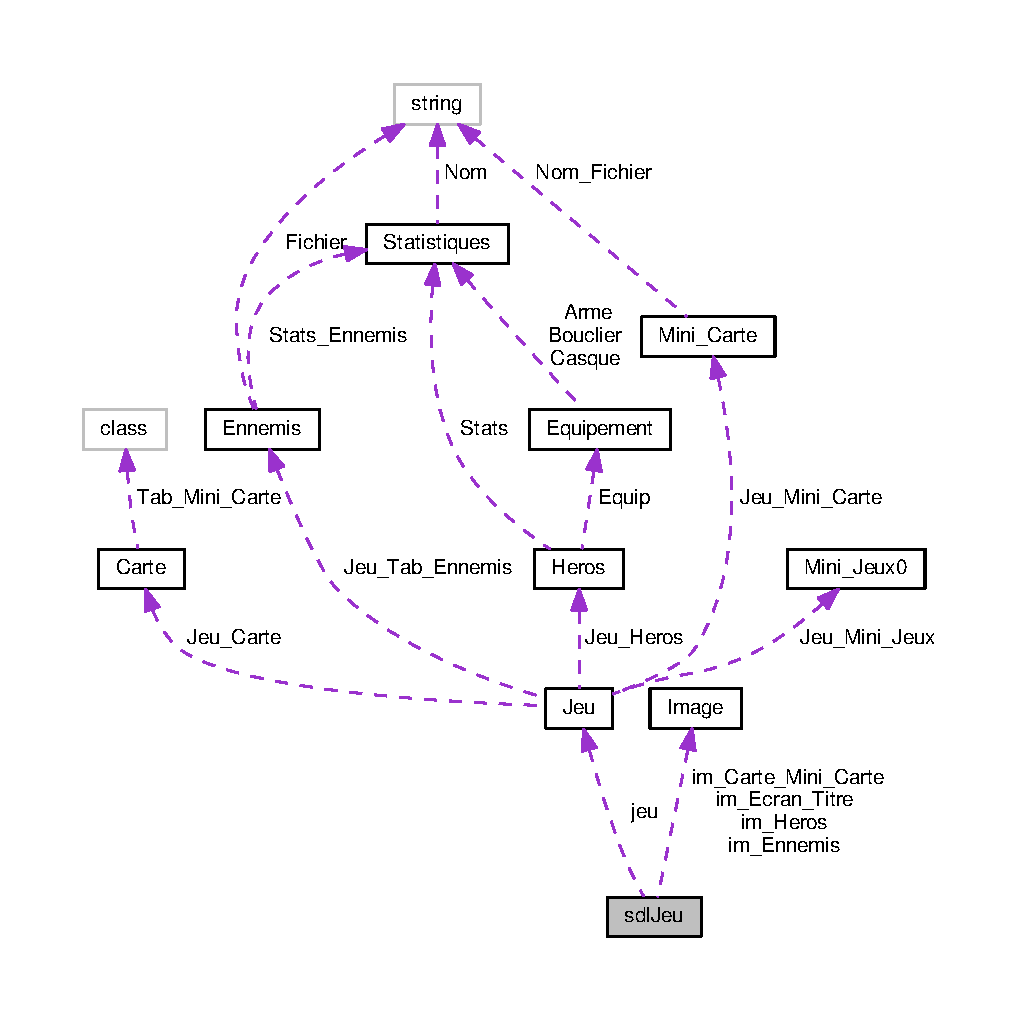
\includegraphics[width=350pt]{classsdlJeu__coll__graph}
\end{center}
\end{figure}
\subsection*{Fonctions membres publiques}
\begin{DoxyCompactItemize}
\item 
\hypertarget{classsdlJeu_a5628835d7efcab056985c3aa3de56836}{void {\bfseries sdl\+Boucle} ()}\label{classsdlJeu_a5628835d7efcab056985c3aa3de56836}

\item 
\hypertarget{classsdlJeu_a191a69d298516350413d423e369d7441}{void {\bfseries sdl\+Aff} (Uint32 t, int repetition\+\_\+touche\+\_\+heros, char touche\+\_\+heros, int pos\+\_\+att\+\_\+mag\+\_\+x, int pos\+\_\+att\+\_\+mag\+\_\+y)}\label{classsdlJeu_a191a69d298516350413d423e369d7441}

\item 
\hypertarget{classsdlJeu_a7cb710d23f671ff25c3a580d3096d7b2}{bool \hyperlink{classsdlJeu_a7cb710d23f671ff25c3a580d3096d7b2}{sdl\+Boucle\+\_\+mini\+\_\+jeux} (string filename)}\label{classsdlJeu_a7cb710d23f671ff25c3a580d3096d7b2}

\begin{DoxyCompactList}\small\item\em lance le mini jeux et gere l'implementation du mini jeux grace aux fonction du jeu et de son mini jeux \end{DoxyCompactList}\item 
\hypertarget{classsdlJeu_a06c22d82de799ed5ccb2acaae8a455dc}{void \hyperlink{classsdlJeu_a06c22d82de799ed5ccb2acaae8a455dc}{sdl\+Aff\+\_\+\+Mini\+\_\+\+Jeux} ()}\label{classsdlJeu_a06c22d82de799ed5ccb2acaae8a455dc}

\begin{DoxyCompactList}\small\item\em utile pour afficher le mini jeux remplace l'ecran du jeu pour le mini jeux utiliser uniquement lors du mini jeux \end{DoxyCompactList}\item 
\hypertarget{classsdlJeu_a2226b2a21cb5999910064eabb7614e09}{void {\bfseries sdl\+Aff\+\_\+\+Carte} ()}\label{classsdlJeu_a2226b2a21cb5999910064eabb7614e09}

\item 
\hypertarget{classsdlJeu_aea5b57a26f7744c38188625944e1e8df}{void {\bfseries Debut\+\_\+\+Partie} ()}\label{classsdlJeu_aea5b57a26f7744c38188625944e1e8df}

\item 
\hypertarget{classsdlJeu_a911fea9f2be914325d94a78c16691ea7}{void {\bfseries Debut\+\_\+\+Jeu} ()}\label{classsdlJeu_a911fea9f2be914325d94a78c16691ea7}

\end{DoxyCompactItemize}
\subsection*{Attributs privés}
\begin{DoxyCompactItemize}
\item 
\hypertarget{classsdlJeu_a43eec470e1819a9df66e019e02928497}{\hyperlink{classJeu}{Jeu} {\bfseries jeu}}\label{classsdlJeu_a43eec470e1819a9df66e019e02928497}

\item 
\hypertarget{classsdlJeu_a9c6b207c8f9108cc52c570f890f20cba}{S\+D\+L\+\_\+\+Window $\ast$ {\bfseries window}}\label{classsdlJeu_a9c6b207c8f9108cc52c570f890f20cba}

\item 
\hypertarget{classsdlJeu_aee1a517fb83b31bf7b19330d652bd7fe}{S\+D\+L\+\_\+\+Renderer $\ast$ {\bfseries renderer}}\label{classsdlJeu_aee1a517fb83b31bf7b19330d652bd7fe}

\item 
\hypertarget{classsdlJeu_aade87bc75844e56cdf868898d26bbb0e}{S\+D\+L\+\_\+\+Color {\bfseries color} = \{0,0,0\}}\label{classsdlJeu_aade87bc75844e56cdf868898d26bbb0e}

\item 
\hypertarget{classsdlJeu_a08dc87030827cd3f6a861af4ddbaf7fd}{T\+T\+F\+\_\+\+Font $\ast$ {\bfseries font}}\label{classsdlJeu_a08dc87030827cd3f6a861af4ddbaf7fd}

\item 
\hypertarget{classsdlJeu_abf097e5a5cfa2a83a165a49a1ac6e950}{S\+D\+L\+\_\+\+Surface $\ast$ {\bfseries texte} = N\+U\+L\+L}\label{classsdlJeu_abf097e5a5cfa2a83a165a49a1ac6e950}

\item 
\hypertarget{classsdlJeu_a852fa68e5f4b504cb3448b8ab9071eba}{S\+D\+L\+\_\+\+Rect {\bfseries rectangle}}\label{classsdlJeu_a852fa68e5f4b504cb3448b8ab9071eba}

\item 
\hypertarget{classsdlJeu_adcebeced03a496240acf5785e2f52dd3}{\hyperlink{classImage}{Image} {\bfseries im\+\_\+\+Heros}}\label{classsdlJeu_adcebeced03a496240acf5785e2f52dd3}

\item 
\hypertarget{classsdlJeu_a3eafc892cc5f11476c61976c1516a59f}{\hyperlink{classImage}{Image} {\bfseries im\+\_\+\+Carte\+\_\+\+Mini\+\_\+\+Carte}}\label{classsdlJeu_a3eafc892cc5f11476c61976c1516a59f}

\item 
\hypertarget{classsdlJeu_a531541bf7f91365fcedb57ba9a970380}{\hyperlink{classImage}{Image} {\bfseries im\+\_\+\+Ennemis}}\label{classsdlJeu_a531541bf7f91365fcedb57ba9a970380}

\item 
\hypertarget{classsdlJeu_a42cb30775a35c957832195352d8a8895}{\hyperlink{classImage}{Image} {\bfseries im\+\_\+\+Ecran\+\_\+\+Titre}}\label{classsdlJeu_a42cb30775a35c957832195352d8a8895}

\end{DoxyCompactItemize}


\subsection{Description détaillée}
La classe gérant le jeu avec un affichage S\+D\+L 

La documentation de cette classe a été générée à partir des fichiers suivants \+:\begin{DoxyCompactItemize}
\item 
src/include/Jeu\+S\+D\+L.\+h\item 
src/cpp/Jeu\+S\+D\+L.\+cpp\end{DoxyCompactItemize}

\hypertarget{classStatistiques}{\section{Référence de la classe Statistiques}
\label{classStatistiques}\index{Statistiques@{Statistiques}}
}


Graphe de collaboration de Statistiques\+:\nopagebreak
\begin{figure}[H]
\begin{center}
\leavevmode
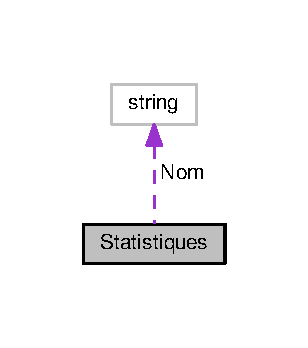
\includegraphics[width=148pt]{classStatistiques__coll__graph}
\end{center}
\end{figure}
\subsection*{Fonctions membres publiques}
\begin{DoxyCompactItemize}
\item 
\hypertarget{classStatistiques_a4ecd522328776fb86ba21d6a3dfe8d70}{\hyperlink{classStatistiques_a4ecd522328776fb86ba21d6a3dfe8d70}{Statistiques} ()}\label{classStatistiques_a4ecd522328776fb86ba21d6a3dfe8d70}

\begin{DoxyCompactList}\small\item\em inititialise a 0 pour toute les stats et un blanc pour le nom \end{DoxyCompactList}\item 
\hypertarget{classStatistiques_acdecb014e7d990998107b74388ee8d8e}{\hyperlink{classStatistiques_acdecb014e7d990998107b74388ee8d8e}{Statistiques} (string nom, unsigned int pv, unsigned int pv\+\_\+max, unsigned int mana, unsigned int mana\+\_\+max, unsigned int xp\+\_\+restant, unsigned int xp\+\_\+donne, unsigned int niveau, unsigned int force, unsigned int intel, unsigned int agilite)}\label{classStatistiques_acdecb014e7d990998107b74388ee8d8e}

\begin{DoxyCompactList}\small\item\em inititialise a partir des valeur entre dans l'ordre \end{DoxyCompactList}\item 
\hyperlink{classStatistiques_a0b3904d9f448c4eb3c88074932c25051}{$\sim$\+Statistiques} ()
\begin{DoxyCompactList}\small\item\em initialise a a partir d'une classe \end{DoxyCompactList}\item 
\hypertarget{classStatistiques_afad913e7a08bb3ae58c0904705415b67}{string \hyperlink{classStatistiques_afad913e7a08bb3ae58c0904705415b67}{get\+\_\+\+Nom} () const }\label{classStatistiques_afad913e7a08bb3ae58c0904705415b67}

\begin{DoxyCompactList}\small\item\em Retourne le nom du porteur de c'est stats. \end{DoxyCompactList}\item 
\hypertarget{classStatistiques_ae439c3b6611afe768407089039386145}{const unsigned int \hyperlink{classStatistiques_ae439c3b6611afe768407089039386145}{get\+\_\+\+Point\+\_\+\+De\+\_\+\+Vie} () const }\label{classStatistiques_ae439c3b6611afe768407089039386145}

\begin{DoxyCompactList}\small\item\em Retourne la valeur des point de vie. \end{DoxyCompactList}\item 
\hypertarget{classStatistiques_aeebd702de918607d509a74dc39901292}{const unsigned int \hyperlink{classStatistiques_aeebd702de918607d509a74dc39901292}{get\+\_\+\+Point\+\_\+\+De\+\_\+\+Vie\+\_\+\+Max} () const }\label{classStatistiques_aeebd702de918607d509a74dc39901292}

\begin{DoxyCompactList}\small\item\em Retourne la valeur des point de vie max. \end{DoxyCompactList}\item 
\hypertarget{classStatistiques_a3ce58d7fa32eec0edde78cfa08fc9690}{const unsigned int \hyperlink{classStatistiques_a3ce58d7fa32eec0edde78cfa08fc9690}{get\+\_\+\+Mana} () const }\label{classStatistiques_a3ce58d7fa32eec0edde78cfa08fc9690}

\begin{DoxyCompactList}\small\item\em Retourne la valeur de la mana actuelle. \end{DoxyCompactList}\item 
\hypertarget{classStatistiques_ac7edbab216440ab35f39c6845e880b11}{const unsigned int \hyperlink{classStatistiques_ac7edbab216440ab35f39c6845e880b11}{get\+\_\+\+Mana\+\_\+\+Max} () const }\label{classStatistiques_ac7edbab216440ab35f39c6845e880b11}

\begin{DoxyCompactList}\small\item\em Retourne la valeur de la mana max possible. \end{DoxyCompactList}\item 
\hypertarget{classStatistiques_accb5cc926122df160d60c877b5f0b79b}{const unsigned int \hyperlink{classStatistiques_accb5cc926122df160d60c877b5f0b79b}{get\+\_\+\+Experience\+\_\+\+Restant} () const }\label{classStatistiques_accb5cc926122df160d60c877b5f0b79b}

\begin{DoxyCompactList}\small\item\em Retourne le nommbre d'experience. \end{DoxyCompactList}\item 
\hypertarget{classStatistiques_a7ffe4b85412dbb43b4c8316a221d19d0}{const unsigned int \hyperlink{classStatistiques_a7ffe4b85412dbb43b4c8316a221d19d0}{get\+\_\+\+Experience\+\_\+\+Donne} () const }\label{classStatistiques_a7ffe4b85412dbb43b4c8316a221d19d0}

\begin{DoxyCompactList}\small\item\em Retourne le nombre d'experience que l'enemis donne. \end{DoxyCompactList}\item 
\hypertarget{classStatistiques_a843d7ebdd796c6893bfa362a7df9e9bc}{const unsigned int \hyperlink{classStatistiques_a843d7ebdd796c6893bfa362a7df9e9bc}{get\+\_\+\+Niveau} () const }\label{classStatistiques_a843d7ebdd796c6893bfa362a7df9e9bc}

\begin{DoxyCompactList}\small\item\em Retourne le niveau actuelle. \end{DoxyCompactList}\item 
\hypertarget{classStatistiques_ab0a704be75b42d629cec33daf3cb4003}{const unsigned int \hyperlink{classStatistiques_ab0a704be75b42d629cec33daf3cb4003}{get\+\_\+\+Force} () const }\label{classStatistiques_ab0a704be75b42d629cec33daf3cb4003}

\begin{DoxyCompactList}\small\item\em Retourne la Statistique Force. \end{DoxyCompactList}\item 
\hypertarget{classStatistiques_a32fb4bdef06a9a16e3a849f4cbd498bf}{const unsigned int \hyperlink{classStatistiques_a32fb4bdef06a9a16e3a849f4cbd498bf}{get\+\_\+\+Intelligence} () const }\label{classStatistiques_a32fb4bdef06a9a16e3a849f4cbd498bf}

\begin{DoxyCompactList}\small\item\em Retourne la Statistique Intelligence. \end{DoxyCompactList}\item 
\hypertarget{classStatistiques_a842c9c8cf791c6fb9fadf5775e346ac8}{const unsigned int \hyperlink{classStatistiques_a842c9c8cf791c6fb9fadf5775e346ac8}{get\+\_\+\+Agilite} () const }\label{classStatistiques_a842c9c8cf791c6fb9fadf5775e346ac8}

\begin{DoxyCompactList}\small\item\em Retourne la Statistique Agilit� \end{DoxyCompactList}\item 
\hypertarget{classStatistiques_af209a1946905d0d7a5f0cb722fb58882}{void \hyperlink{classStatistiques_af209a1946905d0d7a5f0cb722fb58882}{set\+\_\+\+Nom} (string nom)}\label{classStatistiques_af209a1946905d0d7a5f0cb722fb58882}

\begin{DoxyCompactList}\small\item\em Permet d'acc�der nom du porteur de stats. \end{DoxyCompactList}\item 
\hypertarget{classStatistiques_a847eec1508cb5246b506ccffdf1c6d0f}{void \hyperlink{classStatistiques_a847eec1508cb5246b506ccffdf1c6d0f}{set\+\_\+\+Point\+\_\+\+De\+\_\+\+Vie} (unsigned int i)}\label{classStatistiques_a847eec1508cb5246b506ccffdf1c6d0f}

\begin{DoxyCompactList}\small\item\em Permet d'acc�r aux points de vie actuels. \end{DoxyCompactList}\item 
\hypertarget{classStatistiques_a6c9536a38afcd013f2f7659cfab421c7}{void \hyperlink{classStatistiques_a6c9536a38afcd013f2f7659cfab421c7}{set\+\_\+\+Point\+\_\+\+De\+\_\+\+Vie\+\_\+\+Max} (unsigned int i)}\label{classStatistiques_a6c9536a38afcd013f2f7659cfab421c7}

\begin{DoxyCompactList}\small\item\em Permet d'acc�der aux points de vie maximun. \end{DoxyCompactList}\item 
\hypertarget{classStatistiques_a8eab8f9139dc82b515e71103d7aa62b1}{void \hyperlink{classStatistiques_a8eab8f9139dc82b515e71103d7aa62b1}{set\+\_\+\+Mana} (unsigned int i)}\label{classStatistiques_a8eab8f9139dc82b515e71103d7aa62b1}

\begin{DoxyCompactList}\small\item\em Permet d'acc�der aux points de mana actuelle. \end{DoxyCompactList}\item 
\hypertarget{classStatistiques_a73eb98d2d28887809792752e72bfb1f5}{void \hyperlink{classStatistiques_a73eb98d2d28887809792752e72bfb1f5}{set\+\_\+\+Mana\+\_\+\+Max} (unsigned int i)}\label{classStatistiques_a73eb98d2d28887809792752e72bfb1f5}

\begin{DoxyCompactList}\small\item\em Permet d'acc�der aux points de mana maximun. \end{DoxyCompactList}\item 
\hypertarget{classStatistiques_a9a08471f223ff151a8375de70ffea8a0}{void \hyperlink{classStatistiques_a9a08471f223ff151a8375de70ffea8a0}{set\+\_\+\+Experience\+\_\+\+Restant} (unsigned int i)}\label{classStatistiques_a9a08471f223ff151a8375de70ffea8a0}

\begin{DoxyCompactList}\small\item\em Permet d'acc�der a l'experience restant pour le prochain niveau du heros. \end{DoxyCompactList}\item 
\hypertarget{classStatistiques_ac29baea14cb2404cf25530de23cac805}{void \hyperlink{classStatistiques_ac29baea14cb2404cf25530de23cac805}{set\+\_\+\+Experience\+\_\+\+Donne} (unsigned int i)}\label{classStatistiques_ac29baea14cb2404cf25530de23cac805}

\begin{DoxyCompactList}\small\item\em Permet d'acc�der au xp donne par le monstre. \end{DoxyCompactList}\item 
\hypertarget{classStatistiques_ad0a811d25a647679791a2b9803dea4c7}{void \hyperlink{classStatistiques_ad0a811d25a647679791a2b9803dea4c7}{set\+\_\+\+Niveau} (unsigned int i)}\label{classStatistiques_ad0a811d25a647679791a2b9803dea4c7}

\begin{DoxyCompactList}\small\item\em Permet d'acc�der aux niveaux. \end{DoxyCompactList}\item 
\hypertarget{classStatistiques_ac82bd91ca678457004c7c45d699d6334}{void \hyperlink{classStatistiques_ac82bd91ca678457004c7c45d699d6334}{set\+\_\+\+Force} (unsigned int i)}\label{classStatistiques_ac82bd91ca678457004c7c45d699d6334}

\begin{DoxyCompactList}\small\item\em Permet d'acc�der a la stat Force. \end{DoxyCompactList}\item 
\hypertarget{classStatistiques_a76dd38a9eff6ba705bf855074767472a}{void \hyperlink{classStatistiques_a76dd38a9eff6ba705bf855074767472a}{set\+\_\+\+Intelligence} (unsigned int i)}\label{classStatistiques_a76dd38a9eff6ba705bf855074767472a}

\begin{DoxyCompactList}\small\item\em Permet d'acc�der a la stat Intelligence. \end{DoxyCompactList}\item 
\hypertarget{classStatistiques_a4a438f7b2ec1f0650fd0afa222ae2377}{void \hyperlink{classStatistiques_a4a438f7b2ec1f0650fd0afa222ae2377}{set\+\_\+\+Agilite} (unsigned int i)}\label{classStatistiques_a4a438f7b2ec1f0650fd0afa222ae2377}

\begin{DoxyCompactList}\small\item\em Permet d'acc�der a la stat Agilit� \end{DoxyCompactList}\item 
\hypertarget{classStatistiques_af9d9fb83c261f0d685d60cb204fb7efb}{void \hyperlink{classStatistiques_af9d9fb83c261f0d685d60cb204fb7efb}{set\+\_\+\+Statistiques} (\hyperlink{classStatistiques}{Statistiques} stat)}\label{classStatistiques_af9d9fb83c261f0d685d60cb204fb7efb}

\begin{DoxyCompactList}\small\item\em Modifie toutes les statistiques sans effet de bords. \end{DoxyCompactList}\item 
\hypertarget{classStatistiques_a73dd05a5febd2c9765da8802e4b6e228}{void \hyperlink{classStatistiques_a73dd05a5febd2c9765da8802e4b6e228}{Affiche\+\_\+\+Statistiques} () const }\label{classStatistiques_a73dd05a5febd2c9765da8802e4b6e228}

\begin{DoxyCompactList}\small\item\em Affiche les donne membre de la classe statistiques. \end{DoxyCompactList}\item 
\hypertarget{classStatistiques_ab1489e49a99b51b0ecac2b970cdd0a32}{void \hyperlink{classStatistiques_ab1489e49a99b51b0ecac2b970cdd0a32}{Test\+\_\+\+Regression} ()}\label{classStatistiques_ab1489e49a99b51b0ecac2b970cdd0a32}

\begin{DoxyCompactList}\small\item\em Permet de teste si cela fonctionne corectement. \end{DoxyCompactList}\end{DoxyCompactItemize}
\subsection*{Attributs privés}
\begin{DoxyCompactItemize}
\item 
\hypertarget{classStatistiques_a3f6e1f9b8f716bdff742017428677185}{string \hyperlink{classStatistiques_a3f6e1f9b8f716bdff742017428677185}{Nom}}\label{classStatistiques_a3f6e1f9b8f716bdff742017428677185}

\begin{DoxyCompactList}\small\item\em Nom du porteur de ces stats. \end{DoxyCompactList}\item 
\hypertarget{classStatistiques_ae5f23ff7b645a71e38e64a9572752f1e}{unsigned int \hyperlink{classStatistiques_ae5f23ff7b645a71e38e64a9572752f1e}{Point\+\_\+\+De\+\_\+\+Vie}}\label{classStatistiques_ae5f23ff7b645a71e38e64a9572752f1e}

\begin{DoxyCompactList}\small\item\em Points de vie actuelles. \end{DoxyCompactList}\item 
\hypertarget{classStatistiques_ad951396173ee7370faa77c9a13c2284b}{unsigned int \hyperlink{classStatistiques_ad951396173ee7370faa77c9a13c2284b}{Point\+\_\+\+De\+\_\+\+Vie\+\_\+\+Max}}\label{classStatistiques_ad951396173ee7370faa77c9a13c2284b}

\begin{DoxyCompactList}\small\item\em Nombre de point vie que l'on peut avoir au maximun. \end{DoxyCompactList}\item 
\hypertarget{classStatistiques_a2d7bcb3abde843cfc89f22782b9eef77}{unsigned int \hyperlink{classStatistiques_a2d7bcb3abde843cfc89f22782b9eef77}{Mana}}\label{classStatistiques_a2d7bcb3abde843cfc89f22782b9eef77}

\begin{DoxyCompactList}\small\item\em Mana actuelle. \end{DoxyCompactList}\item 
\hypertarget{classStatistiques_a6ed4199dca1684b7b71e82a0bbdcff7b}{unsigned int \hyperlink{classStatistiques_a6ed4199dca1684b7b71e82a0bbdcff7b}{Mana\+\_\+\+Max}}\label{classStatistiques_a6ed4199dca1684b7b71e82a0bbdcff7b}

\begin{DoxyCompactList}\small\item\em Nombre de Mana que l'on peut avoir au maximun. \end{DoxyCompactList}\item 
\hypertarget{classStatistiques_a255b65822177b905d07e1badd9e01bae}{unsigned int \hyperlink{classStatistiques_a255b65822177b905d07e1badd9e01bae}{Experience\+\_\+\+Restant}}\label{classStatistiques_a255b65822177b905d07e1badd9e01bae}

\begin{DoxyCompactList}\small\item\em Nombre d'Experience restant avant le prochain niveau. \end{DoxyCompactList}\item 
\hypertarget{classStatistiques_ade4b7f91c0f6beb0493de01e6789d310}{unsigned int \hyperlink{classStatistiques_ade4b7f91c0f6beb0493de01e6789d310}{Experience\+\_\+\+Donne}}\label{classStatistiques_ade4b7f91c0f6beb0493de01e6789d310}

\begin{DoxyCompactList}\small\item\em Nombre d'experience que les enemis donne. \end{DoxyCompactList}\item 
\hypertarget{classStatistiques_a61ff7ebf9fc2812df7092a38dc75a8c9}{unsigned int \hyperlink{classStatistiques_a61ff7ebf9fc2812df7092a38dc75a8c9}{Niveau}}\label{classStatistiques_a61ff7ebf9fc2812df7092a38dc75a8c9}

\begin{DoxyCompactList}\small\item\em Niveaux actuelle. \end{DoxyCompactList}\item 
\hypertarget{classStatistiques_af9655cd32998ef2a94376aa41992bc9b}{unsigned int \hyperlink{classStatistiques_af9655cd32998ef2a94376aa41992bc9b}{Force}}\label{classStatistiques_af9655cd32998ef2a94376aa41992bc9b}

\begin{DoxyCompactList}\small\item\em Force possed� \end{DoxyCompactList}\item 
\hypertarget{classStatistiques_ad3b445d8256fa5c0c0b820e420d5ac03}{unsigned int \hyperlink{classStatistiques_ad3b445d8256fa5c0c0b820e420d5ac03}{Intelligence}}\label{classStatistiques_ad3b445d8256fa5c0c0b820e420d5ac03}

\begin{DoxyCompactList}\small\item\em Intelligence possed� \end{DoxyCompactList}\item 
\hypertarget{classStatistiques_a58839791bf066d2a7965082fbea2efbd}{unsigned int \hyperlink{classStatistiques_a58839791bf066d2a7965082fbea2efbd}{Agilite}}\label{classStatistiques_a58839791bf066d2a7965082fbea2efbd}

\begin{DoxyCompactList}\small\item\em Agilit� possed� \end{DoxyCompactList}\end{DoxyCompactItemize}


\subsection{Documentation des constructeurs et destructeur}
\hypertarget{classStatistiques_a0b3904d9f448c4eb3c88074932c25051}{\index{Statistiques@{Statistiques}!````~Statistiques@{$\sim$\+Statistiques}}
\index{````~Statistiques@{$\sim$\+Statistiques}!Statistiques@{Statistiques}}
\subsubsection[{$\sim$\+Statistiques}]{\setlength{\rightskip}{0pt plus 5cm}Statistiques\+::$\sim$\+Statistiques (
\begin{DoxyParamCaption}
{}
\end{DoxyParamCaption}
)}}\label{classStatistiques_a0b3904d9f448c4eb3c88074932c25051}


initialise a a partir d'une classe 

Destructeur 

La documentation de cette classe a été générée à partir des fichiers suivants \+:\begin{DoxyCompactItemize}
\item 
src/include/Statistiques.\+h\item 
src/cpp/Statistiques.\+cpp\end{DoxyCompactItemize}

\hypertarget{classWinTXT}{\section{Référence de la classe Win\+T\+X\+T}
\label{classWinTXT}\index{Win\+T\+X\+T@{Win\+T\+X\+T}}
}


une fenêtre texte est un tableau 2\+D de caractères  




{\ttfamily \#include $<$win\+Txt.\+h$>$}

\subsection*{Fonctions membres publiques}
\begin{DoxyCompactItemize}
\item 
\hypertarget{classWinTXT_ad471ddd48d2a7c43acccd1204e419527}{{\bfseries Win\+T\+X\+T} (int dx, int dy)}\label{classWinTXT_ad471ddd48d2a7c43acccd1204e419527}

\item 
\hypertarget{classWinTXT_a1b4cb203533f78bed29498591631f436}{void {\bfseries clear} (char c=' ')}\label{classWinTXT_a1b4cb203533f78bed29498591631f436}

\item 
\hypertarget{classWinTXT_a407cce45e7f81546540f4f8a9b85ce45}{void {\bfseries print} (int x, int y, char c)}\label{classWinTXT_a407cce45e7f81546540f4f8a9b85ce45}

\item 
\hypertarget{classWinTXT_ad021d5fb9862b9ea7985f8cef50451e2}{void {\bfseries print} (int x, int y, char $\ast$c)}\label{classWinTXT_ad021d5fb9862b9ea7985f8cef50451e2}

\item 
\hypertarget{classWinTXT_af83a18827593465fc397983c97b4e886}{void {\bfseries draw} (int x=0, int y=0)}\label{classWinTXT_af83a18827593465fc397983c97b4e886}

\item 
\hypertarget{classWinTXT_a3e8793fd263bb51a62ec8a5e89904c49}{void {\bfseries pause} ()}\label{classWinTXT_a3e8793fd263bb51a62ec8a5e89904c49}

\item 
\hypertarget{classWinTXT_a418c66475403586ac57a80eceb409166}{char {\bfseries get\+Ch} ()}\label{classWinTXT_a418c66475403586ac57a80eceb409166}

\end{DoxyCompactItemize}
\subsection*{Attributs privés}
\begin{DoxyCompactItemize}
\item 
\hypertarget{classWinTXT_aae9dd786d11da5b46de6f4ea3041a0ab}{int \hyperlink{classWinTXT_aae9dd786d11da5b46de6f4ea3041a0ab}{dimx}}\label{classWinTXT_aae9dd786d11da5b46de6f4ea3041a0ab}

\begin{DoxyCompactList}\small\item\em largeur \end{DoxyCompactList}\item 
\hypertarget{classWinTXT_ab94c58aaf938cf5e119553ee918b9a19}{int \hyperlink{classWinTXT_ab94c58aaf938cf5e119553ee918b9a19}{dimy}}\label{classWinTXT_ab94c58aaf938cf5e119553ee918b9a19}

\begin{DoxyCompactList}\small\item\em heuteur \end{DoxyCompactList}\item 
\hypertarget{classWinTXT_ace5ef6c746d586385fcea85073bd1d41}{char $\ast$ \hyperlink{classWinTXT_ace5ef6c746d586385fcea85073bd1d41}{win}}\label{classWinTXT_ace5ef6c746d586385fcea85073bd1d41}

\begin{DoxyCompactList}\small\item\em stocke le contenu de la fenêtre dans un tableau 1\+D mais on y accede en 2\+D \end{DoxyCompactList}\end{DoxyCompactItemize}


\subsection{Description détaillée}
une fenêtre texte est un tableau 2\+D de caractères 

La documentation de cette classe a été générée à partir des fichiers suivants \+:\begin{DoxyCompactItemize}
\item 
src/include/win\+Txt.\+h\item 
src/cpp/win\+Txt.\+cpp\end{DoxyCompactItemize}

%--- End generated contents ---

% Index
\newpage
\phantomsection
\addcontentsline{toc}{chapter}{Index}
\printindex

\end{document}
